\documentclass{pnp_article}

\begin{document}

\SetDocIssue{0.2 (In Progress)}
\SetDocRefNumber{PP-DF-COR-0003}
\SetDocTitle{The CORDET Framework}
\SetDocSubtitle{PUS Extension}
\SetDocAuthor{Alessandro Pasetti}
\SetCheckedBy{Marcel Opprecht}
\maketitle


%---------------------------------------------
% Define Environment for Requirement Tables 
% Par #1: The string identifying the requirement category
% Par #2: The table caption
%---------------------------------------------
\newenvironment{crReq}[2]
{
\begin{longtable}{|l|p{11.8cm}|}
\caption{#2}\label{tab:Req-#1} \\
\hline
\rowcolor{light-gray}
\textbf{Req. ID} & \textbf{Requirement Text}\\
\hline\hline
\endfirsthead
\rowcolor{light-gray}
\textbf{Req. ID} & \textbf{Requirement Text}\\
\hline\hline
\endhead
\DTLforeach*[\DTLiseq{\cat}{#1}]{dbReq}{\cat=Category,\type=Type,\id=Id,\reqText=Text}
{\DTLiffirstrow{}{\\\hline}P-\cat-\id/\type & \textit{\reqText}}\\\hline
}
{\end{longtable}}

%---------------------------------------------
% Define Environment for Adaptation Point Tables 
% Par #1: The string identifying the category to which the AP applies
% Par #2: The table caption
%---------------------------------------------
\newenvironment{crAp}[2]
{
\begin{longtable}{|l|p{4.7cm}|p{6.9cm}|}
\caption{#2}\label{tab:AP-#1} \\
\hline
\rowcolor{light-gray}
\textbf{AP ID} & \textbf{Adaptation Point} & \textbf{Close-Out Value}\\
\hline\hline
\endfirsthead
\rowcolor{light-gray}
\textbf{AP ID} & \textbf{Adaptation Point} & \textbf{Close-Out Value}\\
\hline\hline
\endhead
\DTLforeach*[\DTLiseq{\cat}{#1}]{dbAP}{\cat=Category,\origin=Origin,\id=Id,\ap=AP,\defValue=DefValue}
{\DTLiffirstrow{}{\\\hline}P-\cat-\id & \ap\ (\origin) & \defValue}\\\hline
}
{\end{longtable}}






%---------------------------------------------
% Import tables with requirements and adaptation points
%---------------------------------------------
%\DTLloaddb{dbPus}{PusCompliance.csv}
\DTLloaddb{dbAP}{PusExtensionAP.csv}
%\DTLloaddb{dbCmd}{PusExtensionCmds.csv}
%\DTLloaddb{dbRep}{PusExtensionReps.csv}
\DTLloaddb{dbReq}{PusExtensionReq.csv}
%\DTLloaddb{dbObs}{PusExtensionObs.csv}
%\DTLloaddb{dbPar}{PusExtensionPar.csv}
%\DTLloaddb{dbConst}{PusExtensionConst.csv}
%\DTLloaddb{dbErr}{PusExtensionErr.csv}
%\DTLloaddb{dbEvt}{PusExtensionEvt.csv}
%\DTLloaddb{dbReqVerFailCodes}{PusExtensionReqVerFailCodes.csv}
%\DTLloaddb{dbServ}{PusExtensionServices.csv}

%---------------------------------------------
% Import file with definition of commands and reports
%---------------------------------------------
\def \printOutCmpVerSuccAccRepSpec#1 {
\begin{pnptable}{#1}{Specification of VerSuccAccRep Component}{tab:OutCmpVerSuccAccRepSpec}{Name & VerSuccAccRep(1,1)}
Description & Report generated to mark the successful acceptance of an incoming command \\\hline
Parameters & Packet identifier and packet sequence control of telecommand being acknowledged \\\hline
Discriminant & None \\\hline
Destination & The destination of service 1 reports is set equal to the source of the command being verified \\\hline
Enable Check & Default implementation (report is always enabled) \\\hline
Ready Check & Default implementation (report is always ready) \\\hline
Repeat Check & Default implementation (report is not repeated) \\\hline
Update Action & Default implementation (do nothing) \\\hline
\end{pnptable}}

\def \printOutCmpVerFailedAccRepSpec#1 {
\begin{pnptable}{#1}{Specification of VerFailedAccRep Component}{tab:OutCmpVerFailedAccRepSpec}{Name & VerFailedAccRep(1,2)}
Description & Report generated to mark the acceptance failure of an incoming command \\\hline
Parameters & Packet version number followed by information on the command being acknowledged: packet identifier, packet sequence counter, type, sub-type and discriminant, failure code and one single item of failure data (specific to each failure code).   \\\hline
Discriminant & Failure Identification Code \\\hline
Destination & The destination of service 1 reports is set equal to the source of the command being verified \\\hline
Enable Check & Default implementation (report is always enabled) \\\hline
Ready Check & Default implementation (report is always ready) \\\hline
Repeat Check & Default implementation (report is not repeated) \\\hline
Update Action & Default implementation (do nothing) \\\hline
\end{pnptable}}

\def \printOutCmpVerSuccStartRepSpec#1 {
\begin{pnptable}{#1}{Specification of VerSuccStartRep Component}{tab:OutCmpVerSuccStartRepSpec}{Name & VerSuccStartRep(1,3)}
Description & Report generated to mark the successful start of execution of an incoming command \\\hline
Parameters & Packet identifier and packet sequence control of telecommand being acknowledged \\\hline
Discriminant & None \\\hline
Destination & The destination of service 1 reports is set equal to the source of the command being verified \\\hline
Enable Check & Default implementation (report is always enabled) \\\hline
Ready Check & Default implementation (report is always ready) \\\hline
Repeat Check & Default implementation (report is not repeated) \\\hline
Update Action & Default implementation (do nothing) \\\hline
\end{pnptable}}

\def \printOutCmpVerFailedStartRepSpec#1 {
\begin{pnptable}{#1}{Specification of VerFailedStartRep Component}{tab:OutCmpVerFailedStartRepSpec}{Name & VerFailedStartRep(1,4)}
Description & Report generated to mark the start of execution failure of an incoming command \\\hline
Parameters & Packet version number followed by information on the command being acknowledged: packet identifier, packet sequence counter, type, sub-type and discriminant, failure code and one single item of failure data (specific to each failure code).   \\\hline
Discriminant & Failure Identification Code \\\hline
Destination & The destination of service 1 reports is set equal to the source of the command being verified \\\hline
Enable Check & Default implementation (report is always enabled) \\\hline
Ready Check & Default implementation (report is always ready) \\\hline
Repeat Check & Default implementation (report is not repeated) \\\hline
Update Action & Default implementation (do nothing) \\\hline
\end{pnptable}}

\def \printOutCmpVerSuccPrgrRepSpec#1 {
\begin{pnptable}{#1}{Specification of VerSuccPrgrRep Component}{tab:OutCmpVerSuccPrgrRepSpec}{Name & VerSuccPrgrRep(1,5)}
Description & Report generated to mark the successful completion of an execution step of an incoming command \\\hline
Parameters & Packet identifier and packet sequence control of telecommand being acknowledged \\\hline
Discriminant & None \\\hline
Destination & The destination of service 1 reports is set equal to the source of the command being verified \\\hline
Enable Check & \#TM(1,5) \\\hline
Ready Check & Default implementation (report is always ready) \\\hline
Repeat Check & Default implementation (report is not repeated) \\\hline
Update Action & Default implementation (do nothing) \\\hline
\end{pnptable}}

\def \printOutCmpVerFailedPrgrRepSpec#1 {
\begin{pnptable}{#1}{Specification of VerFailedPrgrRep Component}{tab:OutCmpVerFailedPrgrRepSpec}{Name & VerFailedPrgrRep(1,6)}
Description & Report generated to mark the failure of an execution step of an incoming command \\\hline
Parameters & Packet version number followed by information on the command being acknowledged: packet identifier, packet sequence counter, type, sub-type and discriminant, failure code and one single item of failure data (specific to each failure code); identifier of progress step which failed \\\hline
Discriminant & Failure Identification Code \\\hline
Destination & The destination of service 1 reports is set equal to the source of the command being verified \\\hline
Enable Check & \#TM(1,6) \\\hline
Ready Check & Default implementation (report is always ready) \\\hline
Repeat Check & Default implementation (report is not repeated) \\\hline
Update Action & Default implementation (do nothing) \\\hline
\end{pnptable}}

\def \printOutCmpVerSuccTermRepSpec#1 {
\begin{pnptable}{#1}{Specification of VerSuccTermRep Component}{tab:OutCmpVerSuccTermRepSpec}{Name & VerSuccTermRep(1,7)}
Description & Report generated to mark the successful completion of execution of an incoming command \\\hline
Parameters & Packet identifier and packet sequence control of telecommand being acknowledged \\\hline
Discriminant & None \\\hline
Destination & The destination of service 1 reports is set equal to the source of the command being verified \\\hline
Enable Check & Default implementation (report is always enabled) \\\hline
Ready Check & Default implementation (report is always ready) \\\hline
Repeat Check & Default implementation (report is not repeated) \\\hline
Update Action & Default implementation (do nothing) \\\hline
\end{pnptable}}

\def \printOutCmpVerFailedTermRepSpec#1 {
\begin{pnptable}{#1}{Specification of VerFailedTermRep Component}{tab:OutCmpVerFailedTermRepSpec}{Name & VerFailedTermRep(1,8)}
Description & Report generated to mark the failure to complete execution of an incoming command \\\hline
Parameters & Packet version number followed by information on the command being acknowledged: packet identifier, packet sequence counter, type, sub-type and discriminant, failure code and one single item of failure data (specific to each failure code).   \\\hline
Discriminant & Failure Identification Code \\\hline
Destination & The destination of service 1 reports is set equal to the source of the command being verified \\\hline
Enable Check & Default implementation (report is always enabled) \\\hline
Ready Check & Default implementation (report is always ready) \\\hline
Repeat Check & Default implementation (report is not repeated) \\\hline
Update Action & Default implementation (do nothing) \\\hline
\end{pnptable}}

\def \printOutCmpVerFailedRoutingRepSpec#1 {
\begin{pnptable}{#1}{Specification of VerFailedRoutingRep Component}{tab:OutCmpVerFailedRoutingRepSpec}{Name & VerFailedRoutingRep(1,10)}
Description & Report generated to mark the failure to route an incoming command to its final destination \\\hline
Parameters & Packet version number followed by information on the command whose routing failed: packet identifier, packet sequence counter, type, sub-type and discriminant, and invalid destination \\\hline
Discriminant & None \\\hline
Destination & The destination of service 1 reports is set equal to the source of\newline the command being verified \\\hline
Enable Check & Default implementation (report is always enabled) \\\hline
Ready Check & Default implementation (report is always ready) \\\hline
Repeat Check & Default implementation (report is not repeated) \\\hline
Update Action & Default implementation (do nothing) \\\hline
\end{pnptable}}

\def \printInCmdHkCreHkCmdSpec#1 {
\begin{pnptable}{#1}{Specification of HkCreHkCmd Component}{tab:InCmdHkCreHkCmdSpec}{Name & HkCreHkCmd(3,1)}
Description & Create a housekeeping report structure \\\hline
Parameters & SID, collection interval and identifiers of parameters of the report to be created \\\hline
Discriminant & The structure identifier (SID) of the packet to be created \\\hline
Ready Check & Default implementation (command is always ready) \\\hline
Start Action & Run the procedure Start Action of HkCreate Command of figure \ref{fig:Cmd3s1Start} \\\hline
Progress Action & The following actions are performed:\newline \newline (a) The definition of the new report is added to the RDL, \newline (b) The destination of the new report is equal to the source of the present command\newline (c) The enabled status of the new report is set to 'disabled'\newline (d) The cycle counter of the new report is set to zero\newline (e) The action outcome is set to 'success'\newline (f) The completion outcome is set to 'completed' \\\hline
Termination Action & Default implementation (set action outcome to 'success') \\\hline
Abort Action & Default implementation (set action outcome to 'success') \\\hline
\end{pnptable}}

\def \printInCmdHkCreDiagCmdSpec#1 {
\begin{pnptable}{#1}{Specification of HkCreDiagCmd Component}{tab:InCmdHkCreDiagCmdSpec}{Name & HkCreDiagCmd(3,2)}
Description & Create a diagnostic report structure \\\hline
Parameters & SID, collection interval and identifiers of parameters of the\newline diagnostic report to be created \\\hline
Discriminant & The structure identifier (SID) of the packet to be created \\\hline
Ready Check & Default implementation (command is always ready) \\\hline
Start Action & Run the procedure Start Action of HkCreate Command of figure \ref{fig:Cmd3s1Start} \\\hline
Progress Action & The following actions are performed:\newline \newline (a) The definition of the new report is added to the RDL, \newline (b) The destination of the new report is equal to the source of the present command\newline (c) The enabled status of the new report is set to 'disabled'\newline (d) The cycle counter of the new report is set to zero\newline (e) The action outcome is set to 'success'\newline (f) The completion outcome is set to 'completed' \\\hline
Termination Action & Default implementation (set action outcome to 'success') \\\hline
Abort Action & Default implementation (set action outcome to 'success') \\\hline
\end{pnptable}}

\def \printInCmdHkDelHkCmdSpec#1 {
\begin{pnptable}{#1}{Specification of HkDelHkCmd Component}{tab:InCmdHkDelHkCmdSpec}{Name & HkDelHkCmd(3,3)}
Description & Delete one or more housekeeping report definitions \\\hline
Parameters & List of SIDs of reports whose definition is to be deleted \\\hline
Discriminant & None \\\hline
Ready Check & Default implementation (command is always ready) \\\hline
Start Action & Run the procedure of \ref{fig:Cmd3s3Start} to identify the valid SIDs in the command argument \\\hline
Progress Action & Delete the entries in the RDL corresponding to the SIDs which have been identified as valid by the Start Action and then set the action outcome to 'completed' \\\hline
Termination Action & Default implementation (set action outcome to 'success') \\\hline
Abort Action & Default implementation (set action outcome to 'success') \\\hline
\end{pnptable}}

\def \printInCmdHkDelDiagCmdSpec#1 {
\begin{pnptable}{#1}{Specification of HkDelDiagCmd Component}{tab:InCmdHkDelDiagCmdSpec}{Name & HkDelDiagCmd(3,4)}
Description & Delete one or more diagnostic report definitions \\\hline
Parameters & List of SIDs of reports whose definition is to be deleted \\\hline
Discriminant & None \\\hline
Ready Check & Default implementation (command is always ready) \\\hline
Start Action & Run the procedure of \ref{fig:Cmd3s3Start} to identify the valid SIDs in the command argument \\\hline
Progress Action & Delete the entries in the RDL corresponding to the SIDs which have been identified as valid by the Start Action and then set the action outcome to 'completed' \\\hline
Termination Action & Default implementation (set action outcome to 'success') \\\hline
Abort Action & Default implementation (set action outcome to 'success') \\\hline
\end{pnptable}}

\def \printInCmdHkEnbHkCmdSpec#1 {
\begin{pnptable}{#1}{Specification of HkEnbHkCmd Component}{tab:InCmdHkEnbHkCmdSpec}{Name & HkEnbHkCmd(3,5)}
Description & Enable the periodic generation of one or more housekeeping report structures \\\hline
Parameters & List of SIDs to be enabled  \\\hline
Discriminant & None \\\hline
Ready Check & Default implementation (command is always ready) \\\hline
Start Action & Run the procedure Start Action of Multi-SID Command of figure \ref{fig:Cmd3SidStart} \\\hline
Progress Action & For the entries in the RDL corresponding to the SIDs which have been identified as valid by the Start Action: set enabled flag to true and set the cycle counter to 0. Set the action outcome to 'completed' \\\hline
Termination Action & Default implementation (set action outcome to 'success') \\\hline
Abort Action & Default implementation (set action outcome to 'success') \\\hline
\end{pnptable}}

\def \printInCmdHkDisHkCmdSpec#1 {
\begin{pnptable}{#1}{Specification of HkDisHkCmd Component}{tab:InCmdHkDisHkCmdSpec}{Name & HkDisHkCmd(3,6)}
Description & Disable the periodic generation of one or more housekeeping report structures \\\hline
Parameters & List of SIDs to be disabled \\\hline
Discriminant & None \\\hline
Ready Check & Default implementation (command is always ready) \\\hline
Start Action & Run the procedure Start Action of Multi-SID Command of figure \ref{fig:Cmd3SidStart} \\\hline
Progress Action & Set to false the enable flag of the entries in the RDL corresponding to the SIDs which have been identified as valid by the Start Action and then set the action outcome to 'completed' \\\hline
Termination Action & Default implementation (set action outcome to 'success') \\\hline
Abort Action & Default implementation (set action outcome to 'success') \\\hline
\end{pnptable}}

\def \printInCmdHkEnbDiagCmdSpec#1 {
\begin{pnptable}{#1}{Specification of HkEnbDiagCmd Component}{tab:InCmdHkEnbDiagCmdSpec}{Name & HkEnbDiagCmd(3,7)}
Description & Enable the periodic generation of one or more diagnostic report structures \\\hline
Parameters & List of SIDs to be enabled  \\\hline
Discriminant & None \\\hline
Ready Check & Default implementation (command is always ready) \\\hline
Start Action & Run the procedure Start Action of Multi-SID Command of figure \ref{fig:Cmd3SidStart} \\\hline
Progress Action & For the entries in the RDL corresponding to the SIDs which have been identified as valid by the Start Action: set enabled flag to true and set the cycle counter to 0. Set the action outcome to 'completed' \\\hline
Termination Action & Default implementation (set action outcome to 'success') \\\hline
Abort Action & Default implementation (set action outcome to 'success') \\\hline
\end{pnptable}}

\def \printInCmdHkDisDiagCmdSpec#1 {
\begin{pnptable}{#1}{Specification of HkDisDiagCmd Component}{tab:InCmdHkDisDiagCmdSpec}{Name & HkDisDiagCmd(3,8)}
Description & Disable the periodic generation of one or more diagnostic report structures \\\hline
Parameters & List of SIDs to be disabled  \\\hline
Discriminant & None \\\hline
Ready Check & Default implementation (command is always ready) \\\hline
Start Action & Run the procedure Start Action of Multi-SID Command of figure \ref{fig:Cmd3SidStart} \\\hline
Progress Action & \#TM(3,60 \\\hline
Termination Action & Default implementation (set action outcome to 'success') \\\hline
Abort Action & Default implementation (set action outcome to 'success') \\\hline
\end{pnptable}}

\def \printInCmdHkRepStructHkCmdSpec#1 {
\begin{pnptable}{#1}{Specification of HkRepStructHkCmd Component}{tab:InCmdHkRepStructHkCmdSpec}{Name & HkRepStructHkCmd(3,9)}
Description & This command carries a list of SIDs. For each SID, it triggers the generation of a (3,10) report with the definition of the housekeeping report structure for that SID. \\\hline
Parameters & List of SIDs whose structure is to be reported \\\hline
Discriminant & None \\\hline
Ready Check & Default implementation (command is always ready) \\\hline
Start Action & Run the procedure Start Action of Multi-SID Command of figure \ref{fig:Cmd3SidStart} \\\hline
Progress Action & Run the procedure Progress Action of Report Service 3 Structure of figure \ref{fig:Cmd3s9Prgr} \\\hline
Termination Action & Set action outcome to 'success' if all valid SIDs in the command were successfully processed by the progress action; set it to 'failure' otherwise \\\hline
Abort Action & Default implementation (set action outcome to 'success') \\\hline
\end{pnptable}}

\def \printOutCmpHkRepStructHkRepSpec#1 {
\begin{pnptable}{#1}{Specification of HkRepStructHkRep Component}{tab:OutCmpHkRepStructHkRepSpec}{Name & HkRepStructHkRep(3,10)}
Description & Report carrying the definition of a housekeeping report structure generated in response to a (3,9) command. \\\hline
Parameters & SID of the housekeeping report, flag indicating whether periodic generation of the report is enabled, number of simply commutated parameters in the report and their identifiers, number of super-commutated groups and, for each group, number of parameters in the group and their identifiers \\\hline
Discriminant & Structure Identifier \\\hline
Destination & The destination is set equal to the source of the (3,9) command which triggers the report. \\\hline
Enable Check & The enable status is read from the isEnabled field of the Report Definition corresponding to the report's SID \\\hline
Ready Check & Default implementation (report is always ready) \\\hline
Repeat Check & Default implementation (report is not repeated) \\\hline
Update Action & Load the SID definition from the RDL \\\hline
\end{pnptable}}

\def \printInCmdHkRepStructDiagCmdSpec#1 {
\begin{pnptable}{#1}{Specification of HkRepStructDiagCmd Component}{tab:InCmdHkRepStructDiagCmdSpec}{Name & HkRepStructDiagCmd(3,11)}
Description & This command carries a list of SIDs. For each SID, it triggers the generation of a (3,12) report with the definition of the diagnostic report structure for that SID. \\\hline
Parameters & List of SIDs whose structure is to be reported \\\hline
Discriminant & None \\\hline
Ready Check & Default implementation (command is always ready) \\\hline
Start Action & Run the procedure Start Action of Multi-SID Command of figure \ref{fig:Cmd3SidStart} \\\hline
Progress Action & Run the procedure Progress Action of Report Service 3 Structure of figure \ref{fig:Cmd3s9Prgr} \\\hline
Termination Action & Set action outcome to 'success' if all valid SIDs in the command were successfully processed by the progress action; set it to 'failure' otherwise \\\hline
Abort Action & Default implementation (set action outcome to 'success') \\\hline
\end{pnptable}}

\def \printOutCmpHkRepStructDiagRepSpec#1 {
\begin{pnptable}{#1}{Specification of HkRepStructDiagRep Component}{tab:OutCmpHkRepStructDiagRepSpec}{Name & HkRepStructDiagRep(3,12)}
Description & Report carrying the definition of a diagnostic report structure generated in response to a (3,11) command. \\\hline
Parameters & SID of the diagnostic report, flag indicating whether periodic generation of the report is enabled, number of simply commutated parameters in the report and their identifiers, number of super-commutated groups and, for each group, number of parameters in the group and their identifiers \\\hline
Discriminant & Structure Identifier \\\hline
Destination & The destination is set equal to the source of the (3,11) command which triggers the report. \\\hline
Enable Check & The enable status is read from the isEnabled field of the Report Definition corresponding to the report's SID \\\hline
Ready Check & Default implementation (report is always ready) \\\hline
Repeat Check & Default implementation (report is not repeated) \\\hline
Update Action & Load the SID definition from the RDL \\\hline
\end{pnptable}}

\def \printOutCmpHkRepSpec#1 {
\begin{pnptable}{#1}{Specification of HkRep Component}{tab:OutCmpHkRepSpec}{Name & HkRep(3,25)}
Description & Periodic housekeeping report \\\hline
Parameters & The values of the data items associated to the report's SID in the RDL  \\\hline
Discriminant & Structure Identifier \\\hline
Destination & For pre-defined housekeeping reports, the default destination is HK\_\-DEST. For all other housekeeping reports, the destination is the source of the last (3,5) or (3,7) report enable command. \\\hline
Enable Check & Default implementation (report is always enabled) \\\hline
Ready Check & The Ready Check performs the following actions:\newline \newline (a) If the report's cycle counter in the RDL is equal to the report's period in the RDL, then the report's cycle counter in the RDL is reset to zero\newline (b) If the report's cycle counter in the RDL is equal to zero and the report is enabled in the RDL, then the outcome of the Ready Check is set to: 'ready'; otherwise it is set to 'not ready'\newline (c) The report's cycle counter in the RDL is incremented by 1\newline \newline NB: This logic ensures that the report's cycle counter increments from zero to the report's period and then is reset. The report is 'ready' when its cycle counter is equal to zero. The report's cycle counter is initialized to zero at application's initialization (for pre-defined reports) or when the report is created (for dynamically defined commands) \\\hline
Repeat Check & The Repeat Check returns 'repeat' if the report's SID is defined in the RDL. Otherwise it returns 'no repeat'. \\\hline
Update Action & Load the value of the simply-commutated data items from the data pool and that of the super-commutated data items from the Sampling Buffer associated to the report's SID according to the Report Definition. The report definition is stored in the RDL. \\\hline
\end{pnptable}}

\def \printOutCmpHkDiagRepSpec#1 {
\begin{pnptable}{#1}{Specification of HkDiagRep Component}{tab:OutCmpHkDiagRepSpec}{Name & HkDiagRep(3,26)}
Description & Periodic Diagnostic Report (3,26) \\\hline
Parameters & The values of the data items associated to the report's SID in the RDL \\\hline
Discriminant & Structure Identifier \\\hline
Destination & For pre-defined diagnostic reports, the default destination is HK\_\-DEST. For all other diagnostic reports, the destination is the source of the last (3,5) or (3,7) report enable command. \\\hline
Enable Check & Default implementation (report is always enabled) \\\hline
Ready Check & The Ready Check performs the following actions:\newline \newline (a) If the report's cycle counter in the RDL is equal to the report's period in the RDL, then the report's cycle counter in the RDL is reset to zero\newline (b) If the report's cycle counter in the RDL is equal to zero and the report is enabled in the RDL, then the outcome of the Ready Check is set to: 'ready'; otherwise it is set to 'not ready'\newline (c) The report's cycle counter in the RDL is incremented by 1\newline \newline NB: This logic ensures that the report's cycle counter increments from zero to the report's period and then is reset. The report is 'ready' when its cycle counter is equal to zero. The report's cycle counter is initialized to zero at application's initialization (for pre-defined reports) or when the report is created (for dynamically defined commands) \\\hline
Repeat Check & The Repeat Check returns 'repeat' if the report's SID is defined in the RDL. Otherwise it returns 'no repeat'. \\\hline
Update Action & Load the value of the simply-commutated data items from the data pool and that of the super-commutated data items from the Sampling Buffer associated to the report's SID according to the Report Definition. The report definition is stored in the RDL. \\\hline
\end{pnptable}}

\def \printInCmdHkOneShotHkCmdSpec#1 {
\begin{pnptable}{#1}{Specification of HkOneShotHkCmd Component}{tab:InCmdHkOneShotHkCmdSpec}{Name & HkOneShotHkCmd(3,27)}
Description & Command (3,27) to generate a one-shot housekeeping report \\\hline
Parameters & The list of SIDs for which the one-shot report is to be generated \\\hline
Discriminant & SID to be generated in one-shot mode \\\hline
Ready Check & Return 'command is ready' \\\hline
Start Action & Run the procedure Start Action of Multi-SID Command of figure 9.3 \\\hline
Progress Action & Run the procedure Progress Action of Generate One-Shot Housekeeping Report of figure 9.6 \\\hline
Termination Action & Set action outcome to 'success' if all valid SIDs in the command were successfully processed by the progress action; set it to 'failure' otherwise \\\hline
Abort Action & Do nothing \\\hline
\end{pnptable}}

\def \printInCmdHkOneShotDiagCmdSpec#1 {
\begin{pnptable}{#1}{Specification of HkOneShotDiagCmd Component}{tab:InCmdHkOneShotDiagCmdSpec}{Name & HkOneShotDiagCmd(3,28)}
Description & Command (3,28) to generate a one-shot diagnostic report \\\hline
Parameters & The list of SIDs for which the one-shot report is to be generated \\\hline
Discriminant & SID to be generated in one-shot mode \\\hline
Ready Check & Return 'command is ready' \\\hline
Start Action & Run the procedure Start Action of Multi-SID Command of figure 9.3 \\\hline
Progress Action & Run the procedure Progress Action of Generate One-Shot Housekeeping Report of figure 9.6 \\\hline
Termination Action & Set action outcome to 'success' if all valid SIDs in the command were successfully processed by the progress action; set it to 'failure' otherwise \\\hline
Abort Action & Do nothing \\\hline
\end{pnptable}}

\def \printOutCmpEvtRepaSpec#1 {
\begin{pnptable}{#1}{Specification of EvtRep1 Component}{tab:OutCmpEvtRepaSpec}{Name & EvtRep1(5,1)}
Description & Informative event report \\\hline
Parameters & Event Identifier (EID) acting as discriminant followed by event-specific parameters \\\hline
Discriminant & Event Identifier \\\hline
Destination & The destination of event reports is statically defined and is equal to EVT\_\-DEST. \\\hline
Enable Check & Update service 5 observable nOfDetectedEvt x ('x' is the event severity level) and then retrieve the enable status from the OutRegistry as a function of the report type, sub-type and discriminant \\\hline
Ready Check & Default implementation (report is always ready) \\\hline
Repeat Check & Default implementation (report is not repeated) \\\hline
Update Action & Update service 5 observables: nOfGenEvtRep x, lastEvtEid i, lastEvtTime x ('x' is the event severity level). Note that the event parameters are set by the application which creates the event report at the time it creates it.\newline \newline Set the destination of the event report to EVT\_\-DEST. The destination is a configuration parameter of the PUS Extension. \\\hline
\end{pnptable}}

\def \printOutCmpEvtRepbSpec#1 {
\begin{pnptable}{#1}{Specification of EvtRep2 Component}{tab:OutCmpEvtRepbSpec}{Name & EvtRep2(5,2)}
Description & Low severity event report \\\hline
Parameters & Event Identifier (EID) acting as discriminant followed by event-specific parameters \\\hline
Discriminant & Event Identifier \\\hline
Destination & The destination of event reports is statically defined and is equal to EVT\_\-DEST. \\\hline
Enable Check & Update service 5 observable nOfDetectedEvt x ('x' is the event severity level) and then retrieve the enable status from the OutRegistry as a function of the report type, sub-type and discriminant \\\hline
Ready Check & Default implementation (report is always ready) \\\hline
Repeat Check & Default implementation (report is not repeated) \\\hline
Update Action & Update service 5 observables: nOfGenEvtRep x, lastEvtEid i, lastEvtTime x ('x' is the event severity level). Note that the event parameters are set by the application which creates the event report at the time it creates it.\newline \newline Set the destination of the event report to EVT\_\-DEST. The destination is a configuration parameter of the PUS Extension. \\\hline
\end{pnptable}}

\def \printOutCmpEvtRepcSpec#1 {
\begin{pnptable}{#1}{Specification of EvtRep3 Component}{tab:OutCmpEvtRepcSpec}{Name & EvtRep3(5,3)}
Description & Medium severity event report \\\hline
Parameters & Event Identifier (EID) acting as discriminant followed by event-specific parameters \\\hline
Discriminant & Event Identifier \\\hline
Destination & The destination of event reports is statically defined and is equal to EVT\_\-DEST. \\\hline
Enable Check & Update service 5 observable nOfDetectedEvt x ('x' is the event severity level) and then retrieve the enable status from the OutRegistry as a function of the report type, sub-type and discriminant \\\hline
Ready Check & Default implementation (report is always ready) \\\hline
Repeat Check & Default implementation (report is not repeated) \\\hline
Update Action & Update service 5 observables: nOfGenEvtRep x, lastEvtEid i, lastEvtTime x ('x' is the event severity level). Note that the event parameters are set by the application which creates the event report at the time it creates it.\newline \newline Set the destination of the event report to EVT\_\-DEST. The destination is a configuration parameter of the PUS Extension. \\\hline
\end{pnptable}}

\def \printOutCmpEvtRepdSpec#1 {
\begin{pnptable}{#1}{Specification of EvtRep4 Component}{tab:OutCmpEvtRepdSpec}{Name & EvtRep4(5,4)}
Description & High severity event report  \\\hline
Parameters & Event Identifier (EID) acting as discriminant followed by event-specific parameters \\\hline
Discriminant & Event Identifier \\\hline
Destination & The destination of event reports is statically defined and is equal to EVT\_\-DEST. \\\hline
Enable Check & Update service 5 observable nOfDetectedEvt x ('x' is the event severity level) and then retrieve the enable status from the OutRegistry as a function of the report type, sub-type and discriminant \\\hline
Ready Check & Default implementation (report is always ready) \\\hline
Repeat Check & Default implementation (report is not repeated) \\\hline
Update Action & Update service 5 observables: nOfGenEvtRep x, lastEvtEid i, lastEvtTime x ('x' is the event severity level). Note that the event parameters are set by the application which creates the event report at the time it creates it.\newline \newline Set the destination of the event report to EVT\_\-DEST. The destination is a configuration parameter of the PUS Extension. \\\hline
\end{pnptable}}

\def \printInCmdEvtEnbCmdSpec#1 {
\begin{pnptable}{#1}{Specification of EvtEnbCmd Component}{tab:InCmdEvtEnbCmdSpec}{Name & EvtEnbCmd(5,5)}
Description & Command to enable generation of a list of event identifiers \\\hline
Parameters & List of event identifiers to be enabled  \\\hline
Discriminant & None \\\hline
Ready Check & Default implementation (command is always ready) \\\hline
Start Action & Default implementation (set action outcome to 'success') \\\hline
Progress Action & The event identifiers are processed in sequence and in the order in which they are stored in the event report. Each event identifier is processed in an execution cycle. Each execution cycle counts as a progress step. At each execution, the progress action performs the following actions:\newline \newline (a) If the event identifier is illegal, then: the illegal EID is loaded into verFailData and the Success Outcome is set to VER\_\-ILL\_\-EID\newline (b) If the event identified is legal, then: its enable status is set to 'enabled'; the value of nDisabledEid x ('x' is the severity level of the EID) is decremented; and the Success Outcome of the action is set to 'success'\newline (c) The Completion Outcome of the action is set to 'completed' if all event identifiers carried by the command have been processed; otherwise it is set to 'not completed'.\newline \newline The enable status of the event identifier is stored in the OutRegistry component of the Cordet Framework. \\\hline
Termination Action & The action outcome is set to 'success' if all progress steps were successful. Otherwise, the action outcome is set to VER\_\-ILL\_\-EID and the number of failed progress steps (which corresponds to the number of illegal event identifier in the command) is loaded in verFailData. \\\hline
Abort Action & Default implementation (set action outcome to 'success') \\\hline
\end{pnptable}}

\def \printInCmdEvtDisCmdSpec#1 {
\begin{pnptable}{#1}{Specification of EvtDisCmd Component}{tab:InCmdEvtDisCmdSpec}{Name & EvtDisCmd(5,6)}
Description & Command to disable generation of a list of event identifiers \\\hline
Parameters & List of event identifiers to be disabled  \\\hline
Discriminant & None \\\hline
Ready Check & Default implementation (command is always ready) \\\hline
Start Action & Default implementation (set action outcome to 'success') \\\hline
Progress Action & The event identifiers are processed in sequence and in the order in which they are stored in the event report. Each event identiifier is processed in an execution cycle. Each execution cycle counts as a progress step. At each execution, the progress action performs the following actions:\newline \newline (a) If the event identifier is illegal, then: the illegal EID is loaded into verFailData and the Success Outcome is set to VER\_\-ILL\_\-EID\newline (b) If the event identified is legal, then: its enable status is set to 'disabled'; the value of nDisabledEid x ('x' is the severity level of the EID) is incremented; and the Success Outcome of the action is set to 'success'\newline (c) The Completion Outcome of the action is set to 'completed' if all event identifiers carried by the command have been processed; otherwise it is set to 'not completed'.\newline \newline The enable status of the event identifier is stored in the OutRegistry component of the Cordet Framework. \\\hline
Termination Action & The action outcome is set to 'success' if all progress steps were successful. Otherwise, the action outcome is set to VER\_\-ILL\_\-EID and the number of failed progress steps (which corresponds to the number of illegal event identifier in the command) is loaded in verFailData. \\\hline
Abort Action & Default implementation (set action outcome to 'success') \\\hline
\end{pnptable}}

\def \printInCmdEvtRepDisCmdSpec#1 {
\begin{pnptable}{#1}{Specification of EvtRepDisCmd Component}{tab:InCmdEvtRepDisCmdSpec}{Name & EvtRepDisCmd(5,7)}
Description & This command triggers the generation of a (5,8) report holding the list of disabled event identifiers \\\hline
Parameters & None \\\hline
Discriminant & None \\\hline
Ready Check & Default implementation (command is always ready) \\\hline
Start Action & (a) Compute the number N of (5,8) reports required to hold all the disabled event identifiers. \newline (b) Retrieve N reports of type (5,8)  from the OutFactory\newline (c) Set the action outcome to 'success' if all retrievals are successful; otherwise, generate error report OUTFACTORY FAILED and set the action outcome to VER\_\-REP\_\-CR\_\-FD.\newline \newline NB: The maximum number of (5,8) reports required in response to a single (5,7) commands is given by framework configuration parameter EVT\_\-MAX\_\-N5S8. If N is greater than EVT\_\-MAX\_\-N58, the behaviour of the framework is undefined. \\\hline
Progress Action & Configure the (5,8) reports with a destination equal to the source of the (5,7) command, load them into the OutLoader, and set the action outcome to 'success'. \\\hline
Termination Action & Default implementation (set action outcome to 'success') \\\hline
Abort Action & Default implementation (set action outcome to 'success') \\\hline
\end{pnptable}}

\def \printOutCmpEvtDisRepSpec#1 {
\begin{pnptable}{#1}{Specification of EvtDisRep Component}{tab:OutCmpEvtDisRepSpec}{Name & EvtDisRep(5,8)}
Description & Report generated in response to a (5,7) command carrying the list of disabled Event Identifiers \\\hline
Parameters & The list of disabled event identifiers  \\\hline
Discriminant & None \\\hline
Destination & The destination is set equal to the source of the (5,7) command which triggers the report \\\hline
Enable Check & Default implementation (report is always enabled) \\\hline
Ready Check & Default implementation (report is always ready) \\\hline
Repeat Check & Default implementation (report is not repeated) \\\hline
Update Action & Load the list of disabled event identifiers. First, the event identifiers of severity level 1 are loaded in order of increasing identifier. Then, the  event identifiers of severity level 2 are loaded in order of increasing identifier. And so on for severity levels 3 and 4. If one single (5,8) report is not sufficient to hold all disabled event identifiers, then the event identifiers are loaded in successive (5,8) reports which are triggered by the same (5,7) command. \\\hline
\end{pnptable}}

\def \printInCmdScdEnbTbsCmdSpec#1 {
\begin{pnptable}{#1}{Specification of ScdEnbTbsCmd Component}{tab:InCmdScdEnbTbsCmdSpec}{Name & ScdEnbTbsCmd(11,1)}
Description & Command to enable the time-based schedule execution function \\\hline
Parameters & None \\\hline
Discriminant & None \\\hline
Ready Check & Default implementation (command is always ready) \\\hline
Start Action & Default implementation (set action outcome to 'success') \\\hline
Progress Action & Set the enable status of the time-based schedule execution function to: enabled and start the Time-Based Schedule Execution Procedure of figure \ref{fig:TbsExec} \\\hline
Termination Action & Default implementation (set action outcome to 'success') \\\hline
Abort Action & Default implementation (set action outcome to 'success') \\\hline
\end{pnptable}}

\def \printInCmdScdDisTbsCmdSpec#1 {
\begin{pnptable}{#1}{Specification of ScdDisTbsCmd Component}{tab:InCmdScdDisTbsCmdSpec}{Name & ScdDisTbsCmd(11,2)}
Description & Command to disable the time-based schedule execution function \\\hline
Parameters & None \\\hline
Discriminant & None \\\hline
Ready Check & Default implementation (command is always ready) \\\hline
Start Action & Default implementation (set action outcome to 'success') \\\hline
Progress Action & Set the enable status of the time-based schedule execution function to: disabled and stop the Time-Based Schedule Execution Procedure of figure \ref{fig:TbsExec} \\\hline
Termination Action & Default implementation (set action outcome to 'success') \\\hline
Abort Action & Default implementation (set action outcome to 'success') \\\hline
\end{pnptable}}

\def \printInCmdScdResTbsCmdSpec#1 {
\begin{pnptable}{#1}{Specification of ScdResTbsCmd Component}{tab:InCmdScdResTbsCmdSpec}{Name & ScdResTbsCmd(11,3)}
Description & Command to reset the time-based schedule \\\hline
Parameters & None \\\hline
Discriminant & None \\\hline
Ready Check & Default implementation (command is always ready) \\\hline
Start Action & Default implementation (set action outcome to 'success') \\\hline
Progress Action & (a) Set the enabled status of the time-based schedule execution function to: disabled. \newline (b) Clear all entries in the time-based schedule (TBS). An entry in the TBS is cleared by setting its release time attribute to zero. \newline (c) Delete all sub-schedules and set the number of in use sub-schedules (nOfInUseSubSched) to zero. A sub-schedule is deleted by setting its inUse flag to false.\newline (d) Delete all schedule groups and set the number of in use groups (nOfInUseGroup) to zero. A group is deleted by setting its inUse flag to false. \\\hline
Termination Action & Default implementation (set action outcome to 'success') \\\hline
Abort Action & Default implementation (set action outcome to 'success') \\\hline
\end{pnptable}}

\def \printInCmdScdInsTbaCmdSpec#1 {
\begin{pnptable}{#1}{Specification of ScdInsTbaCmd Component}{tab:InCmdScdInsTbaCmdSpec}{Name & ScdInsTbaCmd(11,4)}
Description & Command to insert one or more time-based activities (TBAs) into the time-based schedule (TBS) \\\hline
Parameters & The sub-schedule to which the TBAs must be added and, for each TBA, the group to which the TBA belongs, its release time and the command which implements the activity \\\hline
Discriminant & None \\\hline
Ready Check & Default implementation (command is always ready) \\\hline
Start Action & Run the procedure Start Action of (11,4) Command of figure \ref{fig:Cmd11s4Start}. This procedure first checks that the sub-schedule identifier has a legal value and then it checks the TBAs in the command. A TBA is rejected if its group identifier is illegal, or if its release time is smaller than the current time plus the time margin, or if the TBS is already full, or if there are insufficient resources to create an InCommand component to encapsulate the command embedded in the activity. \\\hline
Progress Action & For all the activities in the command which have been accepted by the Start Action, the following is done:\newline \newline (a) The TBS is scanned and, when a free slot is found, the activity is loaded in the free slot\newline (b) If the release time of the TBA pointed at by firstTba is larger than the release time of the new TBA, then the value of firstTba is updated to point to the newly inserted TBA\newline (c) The nextTba and prevTba pointers of the newly inserted TBA and of its previous and next TBA are updated to keep the consistency of the TBS\newline (d) The number of scheduled activities (nOfTba) is incremented by 1  \newline (e) The number of activities in the sub-schedule (nOfTbaInSubSched) to which the newly inserted TBA belongs is incremented by 1\newline (f)  The number of activities in the group (nOfTbaInGroup) to which the newly inserted TBA belongs is incremented by 1\newline (g) If the sub-schedule to which the newly inserted TBA belongs was empty, then the number of non-empty sub-schedules (nOfSubSched) is incremented by one\newline \newline After all actvities have been processed, the action outcome is set to: 'completed'. \\\hline
Termination Action & Default implementation (set action outcome to 'success') \\\hline
Abort Action & Default implementation (set action outcome to 'success') \\\hline
\end{pnptable}}

\def \printInCmdScdDelTbaCmdSpec#1 {
\begin{pnptable}{#1}{Specification of ScdDelTbaCmd Component}{tab:InCmdScdDelTbaCmdSpec}{Name & ScdDelTbaCmd(11,5)}
Description & Command to delete one or more time-based activities (TBAs) from the time-based schedule (TBS) \\\hline
Parameters & The number of activities to be deleted and the list of identifiers of the activities to be deleted. Each such identifier is made up of: the identifier of the source, the APID and the sequence count of the request embedded in the activity to be deleted. \\\hline
Discriminant & None \\\hline
Ready Check & Default implementation (command is always ready) \\\hline
Start Action & Run the procedure Start Action of (11,22) Command of figure \ref{fig:Cmd11s22Start}. This procedure iterates over the list of group identifiers in the command and rejects those which are out-of-limit or which are already in use.  \\\hline
Progress Action & For each group identifier which has been accepted by the Start Action, the following is done:\newline \newline (a) The group identifier is marked as in use (its InUse flag is set to true)\newline (b) The enable status of the group identifier is set in accordance with the enable status parameter in the command\newline \newline After all identifiers have been processed, the action outcome is set to: 'completed'. \\\hline
Termination Action & Default implementation (set action outcome to 'success') \\\hline
Abort Action & Default implementation (set action outcome to 'success') \\\hline
\end{pnptable}}

\def \printInCmdScdEnbSubSchedCmdSpec#1 {
\begin{pnptable}{#1}{Specification of ScdEnbSubSchedCmd Component}{tab:InCmdScdEnbSubSchedCmdSpec}{Name & ScdEnbSubSchedCmd(11,20)}
Description & Command to enable one or more time-based sub-schedules \\\hline
Parameters & The number of sub-schedules to be enabled followed by the list of identifiers of the sub-schedules to be enabled \\\hline
Discriminant & None \\\hline
Ready Check & Default implementation (command is always ready) \\\hline
Start Action & Run the procedure of figure \ref{fig:Cmd11s20And21Start}. This procedure checks all the sub-schedule identifiers in the command and rejects those which are invalid (i.e. either outside the range: 1..SCD\_\-N\_\-SUB\_\-TBS or pointing at an empty sub-schuedule). \\\hline
Progress Action & For all the sub-schedule identifiers which have passed the Start Check,set their isSubSchedEnabled attribute to false. \\\hline
Termination Action & Default implementation (set action outcome to 'success') \\\hline
Abort Action & Default implementation (set action outcome to 'success') \\\hline
\end{pnptable}}

\def \printInCmdScdDisSubSchedCmdSpec#1 {
\begin{pnptable}{#1}{Specification of ScdDisSubSchedCmd Component}{tab:InCmdScdDisSubSchedCmdSpec}{Name & ScdDisSubSchedCmd(11,21)}
Description & Command to disable one or more time-based sub-schedules \\\hline
Parameters & The number of sub-schedules to be disabled followed by the list of identifiers of the sub-schedules to be disabled \\\hline
Discriminant & None \\\hline
Ready Check & Default implementation (command is always ready) \\\hline
Start Action & Run the procedure of figure \ref{fig:Cmd11s20And21Start}. This procedure checks all the sub-schedule identifiers in the command and rejects those which are invalid (i.e. either outside the range: 1..SCD\_\-N\_\-SUB\_\-TBS or pointing at an empty sub-schuedule). \\\hline
Progress Action & For all the sub-schedule identifiers which have passed the Start Check,set their isSubSchedEnabled attribute to false. \\\hline
Termination Action & Default implementation (set action outcome to 'success') \\\hline
Abort Action & Default implementation (set action outcome to 'success') \\\hline
\end{pnptable}}

\def \printInCmdScdCreGrpCmdSpec#1 {
\begin{pnptable}{#1}{Specification of ScdCreGrpCmd Component}{tab:InCmdScdCreGrpCmdSpec}{Name & ScdCreGrpCmd(11,22)}
Description & Command to create one or more scheduling groups \\\hline
Parameters & The number of groups to be created and, for each group to be created, its identifier and its initial enable status \\\hline
Discriminant & None \\\hline
Ready Check & Default implementation (command is always ready) \\\hline
Start Action & Run the procedure Start Action of (11,22) Command of figure \ref{fig:Cmd11s22Start}. This procedure iterates over the list of group identifiers in the command and rejects those which are out-of-limit or which are already in use.  \\\hline
Progress Action & For each group identifier which has been accepted by the Start Action, the following is done:\newline \newline (a) The group identifier is marked as in use (its InUse flag is set to true)\newline (b) The enable status of the group identifier is set in accordance with the enable status parameter in the command\newline \newline After all identifiers have been processed, the action outcome is set to: 'completed'. \\\hline
Termination Action & Default implementation (set action outcome to 'success') \\\hline
Abort Action & Default implementation (set action outcome to 'success') \\\hline
\end{pnptable}}

\def \printInCmdScdDelGrpCmdSpec#1 {
\begin{pnptable}{#1}{Specification of ScdDelGrpCmd Component}{tab:InCmdScdDelGrpCmdSpec}{Name & ScdDelGrpCmd(11,23)}
Description & Command to delete one or more scheduling groups \\\hline
Parameters & The number of groups to be delete and the list of their identifiers \\\hline
Discriminant & None \\\hline
Ready Check & Default implementation (command is always ready) \\\hline
Start Action & Run the procedure Start Action of (11,23) Command of figure \ref{fig:Cmd11s23Start}. This procedure iterates over the list of group identifiers (or, if the number of groups to be deleted is equal to zero, over all groups currently in use) and rejects those whose identifiers is out-of-limits or which have activities associated to them. \\\hline
Progress Action & For all group identifiers accepted by the Start Action, the following is done: the group is deleted by setting its InUse flag to false. After all identifiers have been processed, the action outcome is set to: 'completed'.  \\\hline
Termination Action & Default implementation (set action outcome to 'success') \\\hline
Abort Action & Default implementation (set action outcome to 'success') \\\hline
\end{pnptable}}

\def \printInCmdScdEnbGrpCmdSpec#1 {
\begin{pnptable}{#1}{Specification of ScdEnbGrpCmd Component}{tab:InCmdScdEnbGrpCmdSpec}{Name & ScdEnbGrpCmd(11,24)}
Description & Command to enable one or more scheduling groups \\\hline
Parameters & The number of groups to be enabled and the list of their identifiers \\\hline
Discriminant & None \\\hline
Ready Check & Default implementation (command is always ready) \\\hline
Start Action & Run the procedure Start Action of (11,24) and (11,25) Command of figure \ref{fig:Cmd11s24And25Start}. This procedure iterates over the list of group identifiers in the command and rejects those which are not in use. \\\hline
Progress Action & For all group identifiers accepted by the Start Action, the following is done: the isGroupEnabled flag of the group is set to 'Enabled'. After all identifiers have been processed, the action outcome is set to 'completed'. \\\hline
Termination Action & Default implementation (set action outcome to 'success') \\\hline
Abort Action & Default implementation (set action outcome to 'success') \\\hline
\end{pnptable}}

\def \printInCmdScdDisGrpCmdSpec#1 {
\begin{pnptable}{#1}{Specification of ScdDisGrpCmd Component}{tab:InCmdScdDisGrpCmdSpec}{Name & ScdDisGrpCmd(11,25)}
Description & Command to disable one or more scheduling groups \\\hline
Parameters & The number of groups to be disabled and the list of their identifiers \\\hline
Discriminant & None \\\hline
Ready Check & Default implementation (command is always ready) \\\hline
Start Action & Run the procedure Start Action of (11,24) and (11,25) Command of figure \ref{fig:Cmd11s24And25Start}. This procedure iterates over the list of group identifiers in the command and rejects those which are not in use. \\\hline
Progress Action & For all group identifiers accepted by the Start Action, the following is done: the isGroupEnabled flag of the group is set to 'Disabled'. After all identifiers have been processed, the action outcome is set to 'completed'. \\\hline
Termination Action & Default implementation (set action outcome to 'success') \\\hline
Abort Action & Default implementation (set action outcome to 'success') \\\hline
\end{pnptable}}

\def \printInCmdScdRepGrpCmdSpec#1 {
\begin{pnptable}{#1}{Specification of ScdRepGrpCmd Component}{tab:InCmdScdRepGrpCmdSpec}{Name & ScdRepGrpCmd(11,26)}
Description & Command to trigger the generation of a (11,27) report carrying the status of the scheduling groups \\\hline
Parameters & None \\\hline
Discriminant & None \\\hline
Ready Check & Default implementation (command is always ready) \\\hline
Start Action & Retrieve a (11,27) report from the OutFactory. If the retrieval fails, generate error report OUTFACTORY\_\-FAIL and set action outcome to 'failure'. Otherwise, set action outcome to 'success'. \\\hline
Progress Action & Configure the (11,27) report created by the Start Action and load it in the OutLoader. Set the action outcome to 'success' if the load operation is successful and to 'failed' otherwise. \\\hline
Termination Action & Default implementation (set action outcome to 'success') \\\hline
Abort Action & Default implementation (set action outcome to 'success') \\\hline
\end{pnptable}}

\def \printOutCmpScdGrpRepSpec#1 {
\begin{pnptable}{#1}{Specification of ScdGrpRep Component}{tab:OutCmpScdGrpRepSpec}{Name & ScdGrpRep(11,27)}
Description & Report generated in response to a (11,26) command to report the status of the scheduling groups \\\hline
Parameters & The number of currently used scheduling groups and, for each, the identifier and the enable status \\\hline
Discriminant & None \\\hline
Destination & TThe source of the (11,26) command which triggered the generation of the report \\\hline
Enable Check & Default implementation (report is always enabled) \\\hline
Ready Check & Default implementation (report is always ready) \\\hline
Repeat Check & Default implementation (report is not repeated) \\\hline
Update Action & Collect the information about the currently used scheduling groups \\\hline
\end{pnptable}}

\def \printInCmdMonEnbParMonDefCmdSpec#1 {
\begin{pnptable}{#1}{Specification of MonEnbParMonDefCmd Component}{tab:InCmdMonEnbParMonDefCmdSpec}{Name & MonEnbParMonDefCmd(12,1)}
Description & Command to enable one or more monitoring definitions \\\hline
Parameters & The identifiers of the monitoring definitions to be enabled \\\hline
Discriminant & None \\\hline
Ready Check & Default implementation (command is always ready) \\\hline
Start Action & Run the procedure Start Action of Multi-Parameter Monitor Commands of figure \ref{fig:Cmd12s1and2Start} \\\hline
Progress Action & For every parameter monitor identifier in the command which has not been rejected by the Start Action: reset its repetition counter (attribute repCnt) and start its Monitor Procedure. Increment the data pool variable representing the number of enabled parameter monitors by the number of enabled parameter monitors. Set the action outcome to 'completed'. \\\hline
Termination Action & Default implementation (set action outcome to 'success') \\\hline
Abort Action & Default implementation (set action outcome to 'success') \\\hline
\end{pnptable}}

\def \printInCmdMonDisParMonDefCmdSpec#1 {
\begin{pnptable}{#1}{Specification of MonDisParMonDefCmd Component}{tab:InCmdMonDisParMonDefCmdSpec}{Name & MonDisParMonDefCmd(12,2)}
Description & Command to disable one or more monitoring definitions \\\hline
Parameters & The identifiers of the monitoring definitions to be disabled \\\hline
Discriminant & None \\\hline
Ready Check & Default implementation (command is always ready) \\\hline
Start Action & Run the procedure Start Action of Multi-Parameter Monitor Commands of figure \ref{fig:Cmd12s1and2Start} \\\hline
Progress Action & For every valid Parameter Monitor Identifier in the command: stop its Monitor Procedure and set its checking status (attribute checkStatus) to UNCHECKED. Decrement the data pool variable representing the number of enabled parameter monitors by the number of disabled parameter monitors. Set the action outcome to 'completed'. \\\hline
Termination Action & Default implementation (set action outcome to 'success') \\\hline
Abort Action & Default implementation (set action outcome to 'success') \\\hline
\end{pnptable}}

\def \printInCmdMonChgTransDelCmdSpec#1 {
\begin{pnptable}{#1}{Specification of MonChgTransDelCmd Component}{tab:InCmdMonChgTransDelCmdSpec}{Name & MonChgTransDelCmd(12,3)}
Description & Command to change the maximum delay after which the content of the check transition list (CTL) is reported through a (12,12) report \\\hline
Parameters & The new value of the maximum transition reporting delay \\\hline
Discriminant & None \\\hline
Ready Check & Default implementation (command is always ready) \\\hline
Start Action & Set action outcome to 'success' if the argument of the command (the new maximum reporting delay) is a positive integer; otherwise, set the outcome to 'failure' \\\hline
Progress Action & Update the maximum report delay in the data pool with the value in the command \\\hline
Termination Action & Default implementation (set action outcome to 'success') \\\hline
Abort Action & Default implementation (set action outcome to 'success') \\\hline
\end{pnptable}}

\def \printInCmdMonDelAllParMonCmdSpec#1 {
\begin{pnptable}{#1}{Specification of MonDelAllParMonCmd Component}{tab:InCmdMonDelAllParMonCmdSpec}{Name & MonDelAllParMonCmd(12,4)}
Description & Command to delete all parameter monitoring definitions \\\hline
Parameters & None \\\hline
Discriminant & None \\\hline
Ready Check & Default implementation (command is always ready) \\\hline
Start Action & Set action outcome to 'success' if the parameter monitoring function is disabled and if none of the currently defined parameter monitors is attached to a functional monitor which is protected; otherwise set the action outcome to 'failed \\\hline
Progress Action & Delete all entries from the Parameter Monitoring Definition List (PMDL) and delete all entries from the Check Transition List (CTL). Set the data pool variable representing the number of remaining available PMDL entries equal to the size of the PMDL. Set the action outcome to 'completed'. \\\hline
Termination Action & Default implementation (set action outcome to 'success') \\\hline
Abort Action & Default implementation (set action outcome to 'success') \\\hline
\end{pnptable}}

\def \printInCmdMonAddParMonDefCmdSpec#1 {
\begin{pnptable}{#1}{Specification of MonAddParMonDefCmd Component}{tab:InCmdMonAddParMonDefCmdSpec}{Name & MonAddParMonDefCmd(12,5)}
Description & Command to add one or more parameter definitions \\\hline
Parameters & The parameter definitions to be added. Each parameter definition consists of parameter monitor identifier, identifier of parameter to be monitored, description of validity check, repetition counter, description of monitoring check (including identifiers of events to be generated in case of monitoring violation) \\\hline
Discriminant & None \\\hline
Ready Check & Default implementation (command is always ready) \\\hline
Start Action & Run the procedure Start Action of (12,5) Command of figure \ref{fig:Cmd12s5Start} \\\hline
Progress Action & For all parameter monitor definitions which have been accepted by the start action: add the definition to the Parameter Monitor Definition List (PMDL), set the checking status of the new parameter monitor to 'unchecked', reset its repetition counter and phase counter to zero. Decrement the data pool variable representing the number of remaining available entries in the PMDL by the number of added parameter monitors. Set the action outcome to 'completed'. \\\hline
Termination Action & Default implementation (set action outcome to 'success') \\\hline
Abort Action & Default implementation (set action outcome to 'success') \\\hline
\end{pnptable}}

\def \printInCmdMonDelParMonDefCmdSpec#1 {
\begin{pnptable}{#1}{Specification of MonDelParMonDefCmd Component}{tab:InCmdMonDelParMonDefCmdSpec}{Name & MonDelParMonDefCmd(12,6)}
Description & Command to delete one or more parameter monitoring definitions \\\hline
Parameters & The identifiers of the parameter monitors to be deleted \\\hline
Discriminant & None \\\hline
Ready Check & Default implementation (command is always ready) \\\hline
Start Action & Run the procedure Start Action of (12,6) Command of figure \ref{fig:Cmd12s6Start} \\\hline
Progress Action & For all parameter monitor identifiers which have been accepted by the Start Action: delete the parameter monitor from the Parameter Monitor Definition List (PMDL). Increment the data pool variable representing the number of remaining available PMDL entries by the number of deleted parameter monitoring definitions. Set the action outcome to 'completed'. \\\hline
Termination Action & Default implementation (set action outcome to 'success') \\\hline
Abort Action & Default implementation (set action outcome to 'success') \\\hline
\end{pnptable}}

\def \printInCmdMonModParMonDefCmdSpec#1 {
\begin{pnptable}{#1}{Specification of MonModParMonDefCmd Component}{tab:InCmdMonModParMonDefCmdSpec}{Name & MonModParMonDefCmd(12,7)}
Description & Command to modify one or more parameter definitions \\\hline
Parameters & The modified parameter definitions. Each modified parameter definition consists of identifier of parameter monitor, identifier of parameter to be monitored, repetition counter, description of monitoring check (including identifiers of events to be generated in case of monitoring violation) \\\hline
Discriminant & None \\\hline
Ready Check & Default implementation (command is always ready) \\\hline
Start Action & Run the procedure Start Action for (12,7) Command of figure \ref{fig:Cmd12s7Start}  \\\hline
Progress Action & For all the parameter monitors which have been accepted by the Start Action: modify the parameter monitor definition in the PMDL according to the command parameters, set the check status to 'unchecked', reset the repetition counter and the phase counter to zero \\\hline
Termination Action & Default implementation (set action outcome to 'success') \\\hline
Abort Action & Default implementation (set action outcome to 'success') \\\hline
\end{pnptable}}

\def \printInCmdMonRepParMonDefCmdSpec#1 {
\begin{pnptable}{#1}{Specification of MonRepParMonDefCmd Component}{tab:InCmdMonRepParMonDefCmdSpec}{Name & MonRepParMonDefCmd(12,8)}
Description & This command triggers the generation of a (12,9) report carrying one or more parameter monitor definitions \\\hline
Parameters & The identifiers of the parameter monitors whose definitions are to be reported \\\hline
Discriminant & None \\\hline
Ready Check & Default implementation (command is always ready) \\\hline
Start Action & Run the Start Action of (12,8) Command Procedure of figure \ref{fig:Cmd12s8Start}  \\\hline
Progress Action & Configure the (12,9) reports created by the Start Action and load them in the OutLoader. Set the action outcome to 'success' if the load operation is successful and to 'failed' otherwise. \\\hline
Termination Action & Default implementation (set action outcome to 'success') \\\hline
Abort Action & Default implementation (set action outcome to 'success') \\\hline
\end{pnptable}}

\def \printOutCmpMonRepParMonDefRepSpec#1 {
\begin{pnptable}{#1}{Specification of MonRepParMonDefRep Component}{tab:OutCmpMonRepParMonDefRepSpec}{Name & MonRepParMonDefRep(12,9)}
Description & Report generated in response to a (12,8) command to report one or more monitoring definitions. \\\hline
Parameters & The maximum transition reporting delay, and the description of all requested parameter monitors. Each parameter monitor description consists of: parameter monitor identifier, identifier of monitored data item, description of validity condition of parameter monitor (identifier of validity data item, mask and expected value), monitoring interval, monitoring status, repetition number, check type and check-dependent data \\\hline
Discriminant & None \\\hline
Destination & The source of the (12,8) command which triggered the generation of the report \\\hline
Enable Check & Default implementation (report is always enabled) \\\hline
Ready Check & Default implementation (report is always ready) \\\hline
Repeat Check & Default implementation (report is not repeated) \\\hline
Update Action & Default implementation (do nothing) \\\hline
\end{pnptable}}

\def \printInCmdMonRepOutOfLimitsCmdSpec#1 {
\begin{pnptable}{#1}{Specification of MonRepOutOfLimitsCmd Component}{tab:InCmdMonRepOutOfLimitsCmdSpec}{Name & MonRepOutOfLimitsCmd(12,10)}
Description & This command triggers the generation of a (12,11) report holding the parameter monitors which are out of limits \\\hline
Parameters & None \\\hline
Discriminant & None \\\hline
Ready Check & Default implementation (command is always ready) \\\hline
Start Action & Run the Start Action of (12,10) Command Procedure of figure \ref{fig:Cmd12s8Start} \\\hline
Progress Action & Attempt to load the (12,11) report created by the Start Manager in the OutLoader. If the load operation is successful, set the action outcome to 'completed'. Otherwise, release the (12,11) report and set the action outcome to 'failed'. \\\hline
Termination Action & Default implementation (set action outcome to 'success') \\\hline
Abort Action & Default implementation (set action outcome to 'success') \\\hline
\end{pnptable}}

\def \printOutCmpMonRepOutOfLimitsRepSpec#1 {
\begin{pnptable}{#1}{Specification of MonRepOutOfLimitsRep Component}{tab:OutCmpMonRepOutOfLimitsRepSpec}{Name & MonRepOutOfLimitsRep(12,11)}
Description & Report generated in response to a (12,10) command carrying the parameter monitors which are out of limits \\\hline
Parameters & The description of the monitors which are out of limits. Each description consists of: parameter monitor identifier, identifier of monitored data item, check type, current parameter value, value of crossed limit, previous and current checking status, time when the monitoring violation occurred. \\\hline
Discriminant & None \\\hline
Destination & The source of the (12,10) command which triggers the generation of the report \\\hline
Enable Check & Default implementation (report is always enabled) \\\hline
Ready Check & Default implementation (report is always ready) \\\hline
Repeat Check & Default implementation (report is not repeated) \\\hline
Update Action & Default implementation (do nothing) \\\hline
\end{pnptable}}

\def \printOutCmpMonCheckTransRepSpec#1 {
\begin{pnptable}{#1}{Specification of MonCheckTransRep Component}{tab:OutCmpMonCheckTransRepSpec}{Name & MonCheckTransRep(12,12)}
Description & Report carrying the content of the Check Transition List (CTL). \\\hline
Parameters & The entries in the Check Transition List. \\\hline
Discriminant & None \\\hline
Destination & The user of the parameter monitoring function (either a pre-defined application or the source of the most recent command to enable the parameter monitoring function). \\\hline
Enable Check & Default implementation (report is always enabled) \\\hline
Ready Check & Default implementation (report is always ready) \\\hline
Repeat Check & Default implementation (report is not repeated) \\\hline
Update Action & Default implementation (do nothing) \\\hline
\end{pnptable}}

\def \printInCmdMonRepParMonStatCmdSpec#1 {
\begin{pnptable}{#1}{Specification of MonRepParMonStatCmd Component}{tab:InCmdMonRepParMonStatCmdSpec}{Name & MonRepParMonStatCmd(12,13)}
Description & This command triggers the generation of a (12,14) report carrying the status of all parameter monitors \\\hline
Parameters & None \\\hline
Discriminant & None \\\hline
Ready Check & Default implementation (command is always ready) \\\hline
Start Action & Attempt to retrieve an OutComponent of type (12,14) from the OutFactory with a size adequate to hold the status of all currently defined parameter monitors in the PMDL and set the action outcome to 'success' if the operation is successful. If, instead, the OutFactory fails to return the requested OutComponent generate error report OUTFACTORY\_\-FAIL \\\hline
Progress Action & Configure the OutComponent retrieved by the Start Action with the status of all parameter monitors currently defined in the PMD and load it in the OutLoader. Set action outcome to 'success' if the load operation was successful and to 'failed' otherwise. \\\hline
Termination Action & Default implementation (set action outcome to 'success') \\\hline
Abort Action & Default implementation (set action outcome to 'success') \\\hline
\end{pnptable}}

\def \printOutCmpMonRepParMonStatRepSpec#1 {
\begin{pnptable}{#1}{Specification of MonRepParMonStatRep Component}{tab:OutCmpMonRepParMonStatRepSpec}{Name & MonRepParMonStatRep(12,14)}
Description & Report generated in response to a (12,13) report carrying the status of all currently defined parameter monitors \\\hline
Parameters & The checking status of all parameter monitors currently defined in the PDML \\\hline
Discriminant & None \\\hline
Destination & The source of the (12,13) command which triggered the generation of the report \\\hline
Enable Check & Default implementation (report is always enabled) \\\hline
Ready Check & Default implementation (report is always ready) \\\hline
Repeat Check & Default implementation (report is not repeated) \\\hline
Update Action & Default implementation (do nothing) \\\hline
\end{pnptable}}

\def \printInCmdMonEnbParMonFuncCmdSpec#1 {
\begin{pnptable}{#1}{Specification of MonEnbParMonFuncCmd Component}{tab:InCmdMonEnbParMonFuncCmdSpec}{Name & MonEnbParMonFuncCmd(12,15)}
Description & Command to enable the monitoring function \\\hline
Parameters & None \\\hline
Discriminant & None \\\hline
Ready Check & Default implementation (command is always ready) \\\hline
Start Action & Set action outcome to 'success' if the Monitoring Function is disabled (i.e. if the Monitoring Function Procedure is stopped). \\\hline
Progress Action & Start the Monitoring Function Procedure. Set service 12 parameter ServUser equal to the source of this command. Set the enable status of the Parameter Monitoring Function in the data pool to: 'enabled'. Set the action outcome to: 'completed'. \\\hline
Termination Action & Default implementation (set action outcome to 'success') \\\hline
Abort Action & Default implementation (set action outcome to 'success') \\\hline
\end{pnptable}}

\def \printInCmdMonDisParMonFuncCmdSpec#1 {
\begin{pnptable}{#1}{Specification of MonDisParMonFuncCmd Component}{tab:InCmdMonDisParMonFuncCmdSpec}{Name & MonDisParMonFuncCmd(12,16)}
Description & Command to disable the parameter monitoring function \\\hline
Parameters & None \\\hline
Discriminant & None \\\hline
Ready Check & Default implementation (command is always ready) \\\hline
Start Action & Set the action outcome to 'failure' if the Functional Monitoring Function is supported by the application and is enabled. Otherwise set the action outcome to 'success'. \\\hline
Progress Action & Stop the Parameter Monitoring Procedure. Set the enable status of the Parameter Monitoring Function in the data pool to: 'disabled'. Set the action outcome to: 'completed'. \\\hline
Termination Action & Default implementation (set action outcome to 'success') \\\hline
Abort Action & Default implementation (set action outcome to 'success') \\\hline
\end{pnptable}}

\def \printInCmdMonEnbFuncMonCmdSpec#1 {
\begin{pnptable}{#1}{Specification of MonEnbFuncMonCmd Component}{tab:InCmdMonEnbFuncMonCmdSpec}{Name & MonEnbFuncMonCmd(12,17)}
Description & Command to enable the functional monitoring function \\\hline
Parameters & None \\\hline
Discriminant & None \\\hline
Ready Check & Default implementation (command is always ready) \\\hline
Start Action & Set the action outcome to 'failed' if the Parameter Monitoring Function is 'disabled'; otherwise set the action outcome to 'success'. \\\hline
Progress Action & Set the enable status of the Functional Monitoring Function in the data pool to 'enabled'. Set the action outcome to 'completed'. \\\hline
Termination Action & Default implementation (set action outcome to 'success') \\\hline
Abort Action & Default implementation (set action outcome to 'success') \\\hline
\end{pnptable}}

\def \printInCmdMonDisFuncMonCmdSpec#1 {
\begin{pnptable}{#1}{Specification of MonDisFuncMonCmd Component}{tab:InCmdMonDisFuncMonCmdSpec}{Name & MonDisFuncMonCmd(12,18)}
Description & Command to disable the functional monitoring function \\\hline
Parameters & None \\\hline
Discriminant & None \\\hline
Ready Check & Default implementation (command is always ready) \\\hline
Start Action & Default implementation (set action outcome to 'success') \\\hline
Progress Action & Set the enable status of the Functional Monitoring Function in the data pool to 'disabled'. Set the action outcome to 'completed'. \\\hline
Termination Action & Default implementation (set action outcome to 'success') \\\hline
Abort Action & Default implementation (set action outcome to 'success') \\\hline
\end{pnptable}}

\def \printInCmdMonEnbFuncMonDefCmdSpec#1 {
\begin{pnptable}{#1}{Specification of MonEnbFuncMonDefCmd Component}{tab:InCmdMonEnbFuncMonDefCmdSpec}{Name & MonEnbFuncMonDefCmd(12,19)}
Description & Command to enable one or more functional monitoring definitions \\\hline
Parameters & The identifiers of the functional monitors to be enabled \\\hline
Discriminant & None \\\hline
Ready Check & Default implementation (command is always ready) \\\hline
Start Action & Run the procedure Start Action of Multi-Functional Monitor Commands of figure \ref{fig:Cmd12FMonIdStart} \\\hline
Progress Action & For all the valid functional monitor identifiers: enable the functional monitor by setting its isEnabled field in the FDML to true. Set action outcome to 'completed'. Increment the data pool variable representing the number of enabled functional monitors by the number of enabled functional monitors. Set the action outcome to 'completed'. \\\hline
Termination Action & Default implementation (set action outcome to 'success') \\\hline
Abort Action & Default implementation (set action outcome to 'success') \\\hline
\end{pnptable}}

\def \printInCmdMonDisFuncMonDefCmdSpec#1 {
\begin{pnptable}{#1}{Specification of MonDisFuncMonDefCmd Component}{tab:InCmdMonDisFuncMonDefCmdSpec}{Name & MonDisFuncMonDefCmd(12,20)}
Description & Command to disable one ore more functional monitoring definitions \\\hline
Parameters & The identifiers of the functional monitors to be disabled \\\hline
Discriminant & None \\\hline
Ready Check & Default implementation (command is always ready) \\\hline
Start Action & Run the procedure Start Action of Multi-Functional Monitor Commands of figure \ref{fig:Cmd12FMonIdStart} \\\hline
Progress Action & For all the valid functional monitor identifiers: enable the functional monitor by setting its isEnabled field in the FDML to true. Set action outcome to 'completed'. Decrement the data pool variable representing the number of enabled functional monitors by the number of disabled functional monitors. Set the action outcome to 'completed'. \\\hline
Termination Action & Default implementation (set action outcome to 'success') \\\hline
Abort Action & Default implementation (set action outcome to 'success') \\\hline
\end{pnptable}}

\def \printInCmdMonProtFuncMonDefCmdSpec#1 {
\begin{pnptable}{#1}{Specification of MonProtFuncMonDefCmd Component}{tab:InCmdMonProtFuncMonDefCmdSpec}{Name & MonProtFuncMonDefCmd(12,21)}
Description & Command to protect one or more functional monitoring definitions \\\hline
Parameters & The identifiers of the functional monitors to be protected \\\hline
Discriminant & None \\\hline
Ready Check & Default implementation (command is always ready) \\\hline
Start Action & Run the procedure Start Action of Multi-Functional Monitor Commands of figure \ref{fig:Cmd12FMonIdStart} \\\hline
Progress Action & For each functional monitor which has been accepted for execution by the Start Action: set its status to protected in the FMDL. Set the action outcome to 'completed'. \\\hline
Termination Action & Default implementation (set action outcome to 'success') \\\hline
Abort Action & Default implementation (set action outcome to 'success') \\\hline
\end{pnptable}}

\def \printInCmdMonUnprotFuncMonDefCmdSpec#1 {
\begin{pnptable}{#1}{Specification of MonUnprotFuncMonDefCmd Component}{tab:InCmdMonUnprotFuncMonDefCmdSpec}{Name & MonUnprotFuncMonDefCmd(12,22)}
Description & Command to unprotect one or more functional monitoring definitions \\\hline
Parameters & The identifiers of the functional monitors to be unprotected \\\hline
Discriminant & None \\\hline
Ready Check & Default implementation (command is always ready) \\\hline
Start Action & Run the Start Action of Multi-Functional Monitor Command Procedure of figure \ref{fig:Cmd12FMonIdStart} and set action outcome to 'success' \\\hline
Progress Action & For all the valid functional monitor identifiers in the command: unprotect the functional monitor by setting its isProtected flag in the FDML to true. Set action outcome to 'success'. \\\hline
Termination Action & Default implementation (set action outcome to 'success') \\\hline
Abort Action & Default implementation (set action outcome to 'success') \\\hline
\end{pnptable}}

\def \printInCmdMonAddFuncMonDefCmdSpec#1 {
\begin{pnptable}{#1}{Specification of MonAddFuncMonDefCmd Component}{tab:InCmdMonAddFuncMonDefCmdSpec}{Name & MonAddFuncMonDefCmd(12,23)}
Description & Command to add one or more functional monitoring definitions \\\hline
Parameters & The description of the functional monitors to be added. Each description consists of: identifier, description of check validity condition (identifier of validity data item. mask, expected value), the event definition identifier, minimum failing number, list of identifiers of parameter monitors to be associated to the functional monitor.  \\\hline
Discriminant & None \\\hline
Ready Check & Default implementation (command is always ready) \\\hline
Start Action & Run the Start Action of (12,23) Command Procedure of figure \ref{fig:Cmd12s23Start}. \\\hline
Progress Action & For each functional monitor identifier accepted for execution by the Start Action: add the functional monitor definition to the FMDL, set its checking status to 'unchecked', set its enable status to 'disabled', and set its protected status to 'unprotected'. Decrement the data pool variable representing the number of remaining available functional monitors by the number of added functional monitors. Set the action outcome to 'completed'. \\\hline
Termination Action & Default implementation (set action outcome to 'success') \\\hline
Abort Action & Default implementation (set action outcome to 'success') \\\hline
\end{pnptable}}

\def \printInCmdMonDelFuncMonDefCmdSpec#1 {
\begin{pnptable}{#1}{Specification of MonDelFuncMonDefCmd Component}{tab:InCmdMonDelFuncMonDefCmdSpec}{Name & MonDelFuncMonDefCmd(12,24)}
Description & Command to delete one or more functional monitoring definitions to the FMDL \\\hline
Parameters & The identifiers of the functional monitors to be deleted \\\hline
Discriminant & None \\\hline
Ready Check & Default implementation (command is always ready) \\\hline
Start Action & Run the Command (12,24) Start Action Procedure of figure \ref{fig:Cmd12s24Start} \\\hline
Progress Action & For all functional monitors which have been accepted for execution by the Start Action: remove the functional monitor from the FMDL Increment the data pool variable representing the number of remaining available functional monitors by the number of deleted functional monitors. Set the action outcome to 'completed'. \\\hline
Termination Action & Default implementation (set action outcome to 'success') \\\hline
Abort Action & Default implementation (set action outcome to 'success') \\\hline
\end{pnptable}}

\def \printInCmdMonRepFuncMonDefCmdSpec#1 {
\begin{pnptable}{#1}{Specification of MonRepFuncMonDefCmd Component}{tab:InCmdMonRepFuncMonDefCmdSpec}{Name & MonRepFuncMonDefCmd(12,25)}
Description & This command triggers the generation of a (12,26) report carrying the definition of one or more functional monitors \\\hline
Parameters & The identifiers of the functional monitors whose definition is to be reported \\\hline
Discriminant & None \\\hline
Ready Check & Default implementation (command is always ready) \\\hline
Start Action & Run the Start Action of (12,25) Command Procedure of figure \ref{fig:Cmd12s25Start}  \\\hline
Progress Action & Configure the (12,26) reports created by the Start Action and load them in the OutLoader. Set the action outcome to 'success' if the load operation is successful and to "failed' otherwise. \\\hline
Termination Action & Default implementation (set action outcome to 'success') \\\hline
Abort Action & Default implementation (set action outcome to 'success') \\\hline
\end{pnptable}}

\def \printOutCmpMonRepFuncMonDefRepSpec#1 {
\begin{pnptable}{#1}{Specification of MonRepFuncMonDefRep Component}{tab:OutCmpMonRepFuncMonDefRepSpec}{Name & MonRepFuncMonDefRep(12,26)}
Description & Report generated in response to a (12,25) command to carry the definition of some or all functional monitoring definitions \\\hline
Parameters & The description of the functional monitors. Each description consists of: identifier, description of check validity condition (identifier of validity data item. mask, expected value), the protection status, the checking status, the event definition identifier, minimum failing number, list of identifiers of parameter monitors associated to the functional monitor.  \\\hline
Discriminant & None \\\hline
Destination & The source of the (12,25) command which triggered the generation of the report \\\hline
Enable Check & Default implementation (report is always enabled) \\\hline
Ready Check & Default implementation (report is always ready) \\\hline
Repeat Check & Default implementation (report is not repeated) \\\hline
Update Action & Default implementation (do nothing) \\\hline
\end{pnptable}}

\def \printInCmdMonRepFuncMonStatCmdSpec#1 {
\begin{pnptable}{#1}{Specification of MonRepFuncMonStatCmd Component}{tab:InCmdMonRepFuncMonStatCmdSpec}{Name & MonRepFuncMonStatCmd(12,27)}
Description & This command triggers the generation of a (12,28) report carrying the status of all functional monitors \\\hline
Parameters & None \\\hline
Discriminant & None \\\hline
Ready Check & Default implementation (command is always ready) \\\hline
Start Action & Attempt to retrieve an OutComponent of type (12,28) from the OutFactory with a size adequate to hold the status of all currently defined functional monitors in the FMDL and set the action outcome to 'success' if the operation is successful. If, instead, the OutFactory fails to return the requested OutComponent generate error report OUTFACTORY\_\-FAIL   \\\hline
Progress Action & Configure the OutComponent retrieved by the Start Action with the status of all functional monitors currently defined in the FMDL and load it in the OutLoader. Set action outcome to 'success' if the load operation was successful and to 'failed' otherwise. \\\hline
Termination Action & Default implementation (set action outcome to 'success') \\\hline
Abort Action & Default implementation (set action outcome to 'success') \\\hline
\end{pnptable}}

\def \printOutCmpMonRepFuncMonStatRepSpec#1 {
\begin{pnptable}{#1}{Specification of MonRepFuncMonStatRep Component}{tab:OutCmpMonRepFuncMonStatRepSpec}{Name & MonRepFuncMonStatRep(12,28)}
Description & Report generated in response to a (12,27) command carrying the status of all currently defined functional monitors \\\hline
Parameters & The checking status of all functional monitors currently defined in the PDML \\\hline
Discriminant & None \\\hline
Destination & The source of the (12,27) command which triggered the generation of the report \\\hline
Enable Check & Default implementation (report is always enabled) \\\hline
Ready Check & Default implementation (report is always ready) \\\hline
Repeat Check & Default implementation (report is not repeated) \\\hline
Update Action & Default implementation (do nothing) \\\hline
\end{pnptable}}

\def \printOutCmpLptDownFirstRepSpec#1 {
\begin{pnptable}{#1}{Specification of LptDownFirstRep Component}{tab:OutCmpLptDownFirstRepSpec}{Name & LptDownFirstRep(13,1)}
Description & Report carrying the first part of a down-transfer \\\hline
Parameters & Large message transaction identifier, part sequence number and transfer data \\\hline
Discriminant & None \\\hline
Destination & The destination is loaded from parameter lptDest of the LPT Buffer holding the Large Packet to be transferred. This is determined as follows. \newline \newline If the down-transfer is autonomously started by the host application, then its destination is determined by the host application itself. If, instead, the down-transfer is triggered by a (13,129) command, then its destination is the same as the source of the (13,129) command. \\\hline
Enable Check & Report is enabled if the LPT State Machine is in state DOWN\_\-TRANSFER \\\hline
Ready Check & Default implementation (report is always ready) \\\hline
Repeat Check & Default implementation (report is not repeated) \\\hline
Update Action & The following actions are performed:\newline \newline (a) Load the first part of the large packet from the LPT Buffer\newline (b) Set the transaction identifier equal to largeMsgTransId\newline (c) Set the part number equal to partSeqNmb\newline (d) Increment partSeqNmb; and decrement lptRemSize by partSize\newline (e) Set the action outcome to: 'completed' \\\hline
\end{pnptable}}

\def \printOutCmpLptDownInterRepSpec#1 {
\begin{pnptable}{#1}{Specification of LptDownInterRep Component}{tab:OutCmpLptDownInterRepSpec}{Name & LptDownInterRep(13,2)}
Description & Report carrying an intermediate part of a down-transfer \\\hline
Parameters & Large message transaction identifier, part sequence number and\newline transfer data \\\hline
Discriminant & Large Message Trans. Identifier \\\hline
Destination & The destination is loaded from parameter lptDest of the LPT Buffer holding the Large Packet to be transferred. It is determined in the same way as the destination of the (13,1) report which started the down-transfer. \\\hline
Enable Check & Report is enabled if the LPT State Machine is in state DOWN\_\-TRANSFER \\\hline
Ready Check & Default implementation (report is always ready) \\\hline
Repeat Check & Report is repeated as long as lptRemSize is greater than partSize \\\hline
Update Action & The following actions are performed:\newline \newline (a) Load the next part of the large packet from the LPT Buffer\newline (b) Set the transaction identifier equal to largeMsgTransId\newline (c) Set the part number equal to partSeqNmb\newline (d) Increase partSeqNmb \newline (e) Decrement lptRemSize by partSize\newline (f) Set the action outcome to: 'completed' \\\hline
\end{pnptable}}

\def \printOutCmpLptDownLastRepSpec#1 {
\begin{pnptable}{#1}{Specification of LptDownLastRep Component}{tab:OutCmpLptDownLastRepSpec}{Name & LptDownLastRep(13,3)}
Description & Report carrying the last part of a down-transfer \\\hline
Parameters & Large message transaction identifier, part sequence number and transfer data \\\hline
Discriminant & Large Message Trans. Identifier \\\hline
Destination & The destination is loaded from parameter lptDest of the LPT Buffer holding the Large Packet to be transferred. It is determined in the same way as the destination of the (13,1) report which started the down-transfer. \\\hline
Enable Check & Report is enabled if the LPT State Machine is in state DOWN\_\-TRANSFER \\\hline
Ready Check & Default implementation (report is always ready) \\\hline
Repeat Check & Default implementation (report is not repeated) \\\hline
Update Action & The following actions are performed:\newline \newline (a) Load the last part of the large packet from the LPT Buffer\newline (b) Set the transaction identifier equal to largeMsgTransId\newline (c) Set the partnumber equal to partSeqNmb\newline (d) Set the action outcome to: 'completed' \\\hline
\end{pnptable}}

\def \printInCmdLptUpFirstCmdSpec#1 {
\begin{pnptable}{#1}{Specification of LptUpFirstCmd Component}{tab:InCmdLptUpFirstCmdSpec}{Name & LptUpFirstCmd(13,9)}
Description & Command to carry the first part of an up-transfer \\\hline
Parameters & Large message transaction identifier, part sequence number and part data for up-transfer \\\hline
Discriminant & Large Message Trans. Identifier \\\hline
Ready Check & Default implementation (command is always ready) \\\hline
Start Action & The following actions are performed:\newline \newline (a) Determine the identifier of the LPT Buffer for the up-transfer by computing: (x MOD LPT\_\-N\_\-BUF) where `x' is the Large Message Transaction Identifier. \newline (b) Set action outcome to 'success' if the Part Sequence Number is equal to 1 and the LPT State Machine is in state INACTIVE; otherwise set the  action outcome to `failure' \\\hline
Progress Action & The following actions are performed:\newline \newline (a) Send command StartUpTransfer to LPT State Machine\newline (b) Copy the up-transfer data to LPT Buffer and set lptSize to be equal to the amout of copied data\newline (c) Set lptTime to the current time; set partSeqNmb to 1\newline (d) Set lptSrc to the source of the command\newline (e) Set the action outcome to: 'completed' \\\hline
Termination Action & Default implementation (set action outcome to 'success') \\\hline
Abort Action & Default implementation (set action outcome to 'success') \\\hline
\end{pnptable}}

\def \printInCmdLptUpInterCmdSpec#1 {
\begin{pnptable}{#1}{Specification of LptUpInterCmd Component}{tab:InCmdLptUpInterCmdSpec}{Name & LptUpInterCmd(13,10)}
Description & Command to carry an intermediate part of an up-transfer \\\hline
Parameters & Large message transaction identifier, part sequence number and part data for up-transfer \\\hline
Discriminant & Large Message Trans. Identifier \\\hline
Ready Check & Default implementation (command is always ready) \\\hline
Start Action & Run the Procedure Up-Transfer Start Action of figure \ref{fig:Cmd13s10Start}. \\\hline
Progress Action & The following actions are performed:\newline \newline (a) Copy the up-transfer data to LPT Buffer and increment lptSize by the amount of copied data\newline (b) Set  lptTime to the current time\newline (c) Set patSeqNmb to the part sequence number carried by the command \\\hline
Termination Action & Default implementation (set action outcome to 'success') \\\hline
Abort Action & Default implementation (set action outcome to 'success') \\\hline
\end{pnptable}}

\def \printInCmdLptUpLastCmdSpec#1 {
\begin{pnptable}{#1}{Specification of LptUpLastCmd Component}{tab:InCmdLptUpLastCmdSpec}{Name & LptUpLastCmd(13,11)}
Description & Command to carry the last part of an up-transfer \\\hline
Parameters & Large message transaction identifier, part sequence number and\newline part data for up-transfer \\\hline
Discriminant & Large Message Trans. Identifier \\\hline
Ready Check & Default implementation (command is always ready) \\\hline
Start Action & Run the Procedure Up-Transfer Start Action of figure \ref{fig:Cmd13s10Start}. \\\hline
Progress Action & The following actions are performed:\newline \newline (a) Copy the lptSize up-transfer data to LPT Buffer and increment lptSize by the amount of copied data\newline (b) Set current time\newline (c) Set patSeqNmb to the part sequence number carried by the command\newline (d) Send EndUpTransfer command to LPT State Machine\newline (e) Set action outcome to: 'completed' \\\hline
Termination Action & Default implementation (set action outcome to 'success') \\\hline
Abort Action & Default implementation (set action outcome to 'success') \\\hline
\end{pnptable}}

\def \printOutCmpLptUpAbortRepSpec#1 {
\begin{pnptable}{#1}{Specification of LptUpAbortRep Component}{tab:OutCmpLptUpAbortRepSpec}{Name & LptUpAbortRep(13,16)}
Description & Report to notify the abortion of an up-transfer \\\hline
Parameters & Large message transaction identifier and failure reason \\\hline
Discriminant & Large Message Trans. Identifier \\\hline
Destination & The destination is the same as the source of the up-transfer being interrupted \\\hline
Enable Check & Default implementation (report is always enabled) \\\hline
Ready Check & Default implementation (report is always ready) \\\hline
Repeat Check & Default implementation (report is not repeated) \\\hline
Update Action & The large message transaction identifier is taken from parameter largeMsgTransId and the failure reason is read from variable lptFailCode. \\\hline
\end{pnptable}}

\def \printInCmdLptStartDownCmdSpec#1 {
\begin{pnptable}{#1}{Specification of LptStartDownCmd Component}{tab:InCmdLptStartDownCmdSpec}{Name & LptStartDownCmd(13,129)}
Description & Command to start a down-transfer \\\hline
Parameters & Large message transaction identifier \\\hline
Discriminant & Large Message Trans. Identifier \\\hline
Ready Check & Default implementation (command is always ready) \\\hline
Start Action & The following actions are performed:\newline \newline (a) Determine the identifier of the LPT Buffer for the up-transfer by computing: (x MOD LPT\_\-N\_\-BUF) where `x' is the Large Message Transaction Identifier\newline (b) Set action outcome to 'success' if the LPT State Machine is in state INACTIVE; otherwise set the action outcome to `failure' \\\hline
Progress Action & Send command StartDownTransfer to the LPT State Machine \\\hline
Termination Action & Default implementation (set action outcome to 'success') \\\hline
Abort Action & Default implementation (set action outcome to 'success') \\\hline
\end{pnptable}}

\def \printInCmdLptAbortDownCmdSpec#1 {
\begin{pnptable}{#1}{Specification of LptAbortDownCmd Component}{tab:InCmdLptAbortDownCmdSpec}{Name & LptAbortDownCmd(13,130)}
Description & Command to abort a down-transfer \\\hline
Parameters & Large message transaction identifier \\\hline
Discriminant & Large Message Trans. Identifier \\\hline
Ready Check & Default implementation (command is always ready) \\\hline
Start Action & The following actions are performed:\newline \newline (a) Determine the identifier of the LPT Buffer for the up-transfer by computing: (x MOD LPT\_\-N\_\-BUF) where `x' is the Large Message Transaction Identifier\newline (b) Set action outcome to 'success' if the LPT State Machine is in state DOWN\_\-TRANSFER; otherwise set the action outcome to `failure' \\\hline
Progress Action & Send command Abort to the LPT State Machine \\\hline
Termination Action & Default implementation (set action outcome to 'success') \\\hline
Abort Action & Default implementation (set action outcome to 'success') \\\hline
\end{pnptable}}

\def \printInCmdTstAreYouAliveCmdSpec#1 {
\begin{pnptable}{#1}{Specification of TstAreYouAliveCmd Component}{tab:InCmdTstAreYouAliveCmdSpec}{Name & TstAreYouAliveCmd(17,1)}
Description & Command to perform and Are-You-Alive Connection Test \\\hline
Parameters & None \\\hline
Discriminant & None \\\hline
Ready Check & Default implementation (command is always ready) \\\hline
Start Action & Retrieve (17,2) report from OutFactory and set action outcome to 'success' if the retrieval succeeds. If the retrieval fails, generate error report OUTFACTORY FAILED and set outcome of Start Action to 'failed' with failure code VER\_\-REP\_\-CR\_\-FD \\\hline
Progress Action & Configure the (17,2) report with a destination equal to the source of the (17,1), load it in the OutLoader, and then set the action outcome to 'completed' \\\hline
Termination Action & Default implementation (set action outcome to 'success') \\\hline
Abort Action & Default implementation (set action outcome to 'success') \\\hline
\end{pnptable}}

\def \printOutCmpTstAreYouAliveCmdSpec#1 {
\begin{pnptable}{#1}{Specification of TstAreYouAliveCmd Component}{tab:OutCmpTstAreYouAliveCmdSpec}{Name & TstAreYouAliveCmd(17,1)}
Description & Command to perform and Are-You-Alive Connection Test \\\hline
Parameters & None \\\hline
Discriminant & None \\\hline
Destination & The application providing the test service \\\hline
Enable Check & Default implementation \\\hline
Ready Check & Default implementation \\\hline
Repeat Check & Default implementation \\\hline
Update Action & Default implementation \\\hline
\end{pnptable}}

\def \printOutCmpTstAreYouAliveRepSpec#1 {
\begin{pnptable}{#1}{Specification of TstAreYouAliveRep Component}{tab:OutCmpTstAreYouAliveRepSpec}{Name & TstAreYouAliveRep(17,2)}
Description & Report generated in response to a (17,1) command requesting an Are-You-Alive Connection Test \\\hline
Parameters & None \\\hline
Discriminant & None \\\hline
Destination & The source of the (17,1) command which triggered the report \\\hline
Enable Check & Default implementation (report is always enabled) \\\hline
Ready Check & Default implementation (report is always ready) \\\hline
Repeat Check & Default implementation (report is not repeated) \\\hline
Update Action & Default implementation (do nothing) \\\hline
\end{pnptable}}

\def \printInRepTstAreYouAliveRepSpec#1 {
\begin{pnptable}{#1}{Specification of TstAreYouAliveRep Component}{tab:InRepTstAreYouAliveRepSpec}{Name & TstAreYouAliveRep(17,2)}
Description & Report generated in response to a (17,1) command requesting an Are-You-Alive Connection Test \\\hline
Parameters & None \\\hline
Discriminant & None \\\hline
Acceptance Check & Default implementation \\\hline
Update Action & Set AreYouAliveSrc to the source of the report \\\hline
\end{pnptable}}

\def \printInCmdTstConnectCmdSpec#1 {
\begin{pnptable}{#1}{Specification of TstConnectCmd Component}{tab:InCmdTstConnectCmdSpec}{Name & TstConnectCmd(17,3)}
Description & Command to perform and On-Board Connection Test.  \\\hline
Parameters & Identifier of application with which the connection test is done \\\hline
Discriminant & None \\\hline
Ready Check & Default implementation (command is always ready) \\\hline
Start Action & Run the procedure Start Action of (17,3) Command of figure \ref{fig:Cmd17s3Start}) \\\hline
Progress Action & Run the procedure Progress Action of (17,3) Command of figure \ref{fig:Cmd17s3Start}) \\\hline
Termination Action & Set action outcome to 'success' if the (17,4) report was issued and to 'failure' otherwise with failure code VER\_\-TST\_\-TO \\\hline
Abort Action & Default implementation (set action outcome to 'success') \\\hline
\end{pnptable}}

\def \printOutCmpTstConnectRepSpec#1 {
\begin{pnptable}{#1}{Specification of TstConnectRep Component}{tab:OutCmpTstConnectRepSpec}{Name & TstConnectRep(17,4)}
Description & Report generated in response to a (17,3) command requesting a On-Board Connection Test \\\hline
Parameters & Identifier of application with which the connection test was done \\\hline
Discriminant & None \\\hline
Destination & The source of the (17,3) command which triggered the report \\\hline
Enable Check & Default implementation (report is always enabled) \\\hline
Ready Check & Default implementation (report is always ready) \\\hline
Repeat Check & Default implementation (report is not repeated) \\\hline
Update Action & Default implementation (do nothing) \\\hline
\end{pnptable}}

\def \printInCmdDumSampleaSpec#1 {
\begin{pnptable}{#1}{Specification of DumSample1 Component}{tab:InCmdDumSampleaSpec}{Name & DumSample1(255,1)}
Description & Sample command used for testing purposes. The outcome of all its actions and checks can be set by setting user-commandable flags. Its actions increment the value of user-observable counters.  \\\hline
Parameters & None \\\hline
Discriminant & None \\\hline
Ready Check & The Ready Check returns the value of an internal flag (the Ready Flag) whose value is set through function <code>::CrFwInCmdSample1SetReadyFlag</code>. \\\hline
Start Action & This action sets the outcome to the value of an internal counter (the Start Action Outcome Counter) whose value is set through function <code>::CrFwInCmdSample1SetStartActionOutcome</code> and it increments the value of a counter (the Start Action Counter) whose value is read through function <code>::CrFwInCmdSample1GetStartActionCounter</code>. \\\hline
Progress Action & This action:\newline  (a) Sets the outcome to the value of an internal counter (the Progress Action Outcome Counter) whose value is set through function <code>::CrFwInCmdSample1SetProgressActionOutcome</code>, and\newline  (b) It increments the progress step identifier if the progress step flag is set (its value is controlled through function <code>::CrFwInCmdSample1SetProgressActionFlag</code>. \\\hline
Termination Action & This actions sets the outcome to the value of an internal counter (the Termination Action Outcome Counter) whose value is set through function <code>::CrFwInCmdSample1SetTerminationActionOutcome</code> and it increments the value of a counter (the Termination Action Counter) whose value is read through function <code>::CrFwInCmdSample1GetTerminationActionCounter</code>. \\\hline
Abort Action & This action sets the outcome to the value of an internal counter (the Abort Action Outcome Counter) whose value is set through function <code>::CrFwInCmdSample1SetAbortActionOutcome</code> and it increments the value of a counter (the Abort Action Counter) whose value is read through function <code>::CrFwInCmdSample1GetAbortActionCounter</code>. \\\hline
\end{pnptable}}




% =======================================================================
%\listofchanges
\tableofcontents
\listoffigures
\listoftables


%==========================================================================================
\section{Change History}

This section lists the changes made in the current and previous revisions. Changes are classified according to their type. The change type is identified in the second column in the table according to the following convention:

\begin{itemize}
\item "\textbf{E}": Editorial or stylistic change
\item "\textbf{L}": Clarification of existing text
\item "\textbf{D}": A requirement has in whole or in part been deleted
\item "\textbf{C}": A requirement has been modified
\item "\textbf{N}": A new requirement has been introduced
\item "\textbf{T}": A TBD or TBC has been resolved
\end{itemize}

Text which is new or has been modified in the current revision is in red font. If a figure has been modified, then its caption is in red font. Section header numbers do not change from one revision to the next (but new sections may, of course, be introduced). However, figure and table numbers may change and these changes are not tracked. Changes in the appendices are not tracked as they are consequences of changes in the main body of the document.

\begin{longtable}{|c|c|p{10cm}|}
\caption{Detailed List of Changes in Issue 0.1} \\
\hline
\rowcolor{light-gray}
\textbf{Sec} & \textbf{Type} & \textbf{Description of Change} \\
\hline\hline
\endfirsthead
\rowcolor{light-gray}
\textbf{Sec} & \textbf{Type} & \textbf{Description of Change} \\
\hline\hline
\endhead
n.a. & L & This is the first release of this document \\
\hline
\end{longtable}






\newpage

%==========================================================================================
\section{Applicable and Reference Documents}

The documents in table \ref{tab:appDoc} form an integral part of the present document. The documents in table \ref{tab:refDoc} are referenced in the present document and are for information only.

\begin{longtable}{|c|p{11cm}|}
\caption{Applicable Documents} \label{tab:appDoc}\\
\hline
\rowcolor{light-gray}
\textbf{ID} & \textbf{Title, Reference Number, Revision Number} \\
\hline\hline
\endfirsthead
\rowcolor{light-gray}
\textbf{ID} & \textbf{Title, Reference Number, Revision Number} \\
\hline\hline
\endhead
[CR-SP] & The CORDET Framework - Specification, PP-DF-COR-00002, Revision 1.6, P\&P Software GmbH, Switzerland, 2012, Available from: \url{www.pnp-software.com/cordetfw} \\
\hline
[FW-SP] & The Framework Profile, PP-DF-COR-00001, Revision 1.3, P\&P Software GmbH, Switzerland, 2012, Available from: \url{www.pnp-software.com/fwprofile} \\
\hline
[PS-SP] & Ground Systems and Operations – Telemetry and Telecommand Packet Utilization Standard, ECSS-E-70-41C, April 2016, European Cooperation for Space Standardization (ECSS) \\
\hline
[PX-SP] & The present document \\
\hline
\end{longtable}

\begin{longtable}{|c|p{11cm}|}
\caption{Reference Documents} \label{tab:refDoc}\\
\hline
\rowcolor{light-gray}
\textbf{ID} & \textbf{Title, Reference Number, Revision Number} \\
\hline\hline
\endfirsthead
\rowcolor{light-gray}
\textbf{ID} & \textbf{Title, Reference Number, Revision Number} \\
\hline\hline
\endhead
[PS-WEB] & The CORDET Framework Project Web Site, \url{www.pnp-software.com/cordetfw} \\
\hline
\end{longtable}


\newpage


%==========================================================================================
\section{Introduction}
The CORDET Framework is a software framework for service-oriented embedded applications. It is specified in [CR-SP] as a set of components to manage the services which an application provides to other applications and uses from other applications. A C-language implementation of this specification is available from [CR-WEB].

The CORDET Framework only covers the management of generic services but does not specify any concrete services. The service concept of the CORDET Framework is the same as the service concept of the \textit{Packet Utilization Standard} (PUS). The PUS is an application-level interface standard for space-based distributed systems. It is defined in [PS-SP].

The PUS pre-defines a number of services. This document extends the CORDET Framework to support a subset of those services. The document specifies the components which implements them. The components are specified by providing their behavioural model. The behavioural models are defined using the FW Profile. The FW Profile is a UML profile for reusable software components. It is defined in [FW-SP].

The set of components specified in this document are called the \textit{PUS Extension of the CORDET Framework}. When there is no danger of ambiguity, the shorter names "framework extension" or "PUS extension" are also used as synonyms of PUS Extension of the CORDET Framework.

In terms of the classical software lifecycle, the specification presented in this document is at the level of software requirements in the sense that it defines a complete and unambiguous logical model of the components implementing the PUS extension of the CORDET Framework.

\textbf{This document assumes the reader to be familiar with the specification of the CORDET Framework in [CR-SP]}. 

\subsection{Scope of CORDET Framework}\label{sec:ScopeCrFw}
A \textit{CORDET service} is a set of logically and functionally related capabilities that an application offers to other applications. The CORDET Service concept sees an application as a \textit{provider of services} to other applications and as a \textit{user of services} from other applications (see figure \ref{fig:ServConcept}).

\pnpfigure[scale=0.4]{Applications as Providers and Users of Services}{fig:ServConcept}{ServConcept.png}

The user of a service controls the service by sending \textit{commands} to the service provider. A command is a data exchange between a service user and a service provider to control the execution of a particular activity within the service provider. 

The provider of a service sends \textit{reports} to the user of the service. A report is a data exchange between a service provider (the report initiator) and a service user to provide information relating to the execution of a service activity.

Thus, a service consists of a set of commands which the user of the service sends to the provider of the service and of a set of reports which the service provider sends back to its user. A command defines actions to be executed by the service provider. A report encapsulates information about the internal state of the service provider.

Against this background, the CORDET Framework of [CR-SP] fulfils two objectives:

\begin{itemize}
\item{} It provides a formal definition of the abstract command concept and of the abstract report concept by building behavioural models of commands and reports which:
	\begin{itemize}
	\item capture the aspects of the behaviour of commands and reports which are common to all commands and reports, and
	\item identify the adaptation points where service- and implementation-specific behaviour can be added.
	\end{itemize}
\item{} It specifies the component (the \textit{CORDET Components}) which implement the abstract command and report concept.
\end{itemize}

The CORDET Components cover, on the service user side, the sending of commands and the reception and distribution of reports and, on the service provider side, the processing of incoming commands and the generation of reports but do not cover the implementation of any concrete services. 

%--------------------------------------------------------------------------------
\subsection{Scope of PUS Extension of CORDET Framework}\label{sec:ScopePusExt}
Developers of a CORDET application are expected to deploy the CORDET components and complement them with application-specific components which implement the services of interest to them. The PUS extension of the CORDET Framework facilitates the task of application developers by offering them a set of pre-defined components which implement a set of \textit{Standard Services}. A standard service in this context is a service which implements commonly used functions within a certain domain. 

The standard services of the PUS Extension are taken from the Packet Utilization Standard (PUS) of [PS-SP]. The target domain of the PUS Extension is therefore that of space-borne service-provider applications but it is worth stressing that the set of services selected from the PUS are those which are least dependent on the space context and it is therefore expected that the services implemented by the PUS Extension may be of interest to other application domains.

The standard services are defined by defining their commands and reports and the commands and reports are defined as specializations of the abstract command and report concepts of the CORDET Framework. Thus, a standard service is defined by “closing” the adaptation points identified in the abstract command and report concepts.

The CORDET Framework is ultimately intended to foster reuse (at both specification and implementation level) in the field of service-oriented embedded applications. The reuse model it promotes is illustrated in figure \ref{fig:HierarchicalDefServ}. At the top layer, there is the abstract definition of commands and reports of the CORDET Framework of [CR-SP]. This definition is entirely generic and applicable to all services in all applications. At the intermediate level, standard services are defined which capture concrete behaviour which is common to a large number of applications. The present document specifies one such set of standard services. Finally, at the bottom level, end-applications define their own services which are entirely specific to their needs. The application-level services may be either taken over from the standard services or they may be created as instantiations of the generic service concept (if they are entirely application-specific).

Note that the PUS Extension of the CORDET Framework specifies several services. These services are specified to be independent of each other so that the user may choose only a subset of these services. Similarly, each service is specified in terms of the commands and reports which implement it. Dependencies among the commands and reports of a service are minimized so that users may be free to import into their application just a subset of the commands and reports of a given service.

\begin{figure}[ht]
 \centering
 \includegraphics[scale=0.3,keepaspectratio=true]{HierarchicalDefServ.png}
 \caption{Hierarchical Definition of Services}
 \label{fig:HierarchicalDefServ}
\end{figure}


%---------------------------------------------------------------------------------
\subsubsection{Overview of Supported Services}
Table \ref{tab:supportedServ} lists the services supported by the PUS Extension of the CORDET Framework. The first column gives the service type identifier. The last column points to the section in this document where the support for the service is specified.

\begin{pnptable}{|c|>{\raggedright\arraybackslash}p{6cm}|c|}{Services Supported by PUS Extension}{tab:supportedServ}{\textbf{N} &\textbf{Service} & \textbf{Section}}
1 & Request Verification Service & \ref{sec:serv1} \\
\hline
3 & Housekeeping Service & \ref{sec:serv3} \\
\hline
5 & Event Reporting Service & \ref{sec:serv5} \\
\hline
12 & On-Board Monitoring Service & \ref{sec:serv12} \\
\hline
13 & Large Packet Transfer Service & \ref{sec:serv13} \\
\hline
17 & Test Service & \ref{sec:serv17} \\
\hline
19 & Event Action Service & \ref{sec:serv19} \\
\hline
\end{pnptable}


%------------------------------------------------------------------------------------
\subsection{Specification Format} 
This document specifies the PUS Extension of the CORDET Framework. The framework is specified by defining its requirements. The requirements of the framework are of four types:

\begin{itemize}
\item{} \textit{Standard Requirements} which define a desired feature of the framework extension. They are analogous in scope and format to the user requirements of a conventional (non-framework) application.
\item{} \textit{Adaptation Requirement} which define the points where a component offered by the framework extension can be extended by the application developers. In some cases, the definition of an adaptation point is accompanied by the definition of the default options offered by the framework extension for that adaptation point.  
\item{} \textit{Use Constraint Requirements} which define the constraints on how the components offered by the framework extension may be used by application developers.
\item{} \textit{Property Requirements} which define behavioural properties which are guaranteed to hold on all applications which: (a) are instantiated from the CORDET Framework and its extension by closing their adaptation points, and (b) comply with the framework's use constraints.
\end{itemize}

To each framework requirement an \textit{identifier} is attached.
The requirement identifier takes the following form: x-y/t where 'x' is an acronym identifying the function to which the requirement applies; 'y' is a unique identifier within that function; and 't' identifies the requirement type. 
The type is designated by one single letter as follows: 'S' for the Standard Requirements, 'A' for the Adaptation Requirements, 'C' for the Use Constraint Requirements and 'P' for the Property Requirements.

The specification of the framework extension includes a \textit{behavioural model} of the framework which describes its behaviour and identifies the adaptation points where application developers can extend this behaviour to match their requirements.  

The behavioural model of the framework extension is defined using the FW Profile of [FW-PS]. It therefore consists of a set of \textit{state machines} (represented as state charts) and \textit{procedures} (represented as  activity diagrams). Familiarity with the FW Profile is essential for a full understanding of the framework requirements.

Wherever possible, the framework extension requirements simply make the state machines and procedures applicable. In other words, the state charts representing state machines and the activity diagrams representing procedures are treated as normative and no attempt is made to translate them into a comprehensive set of equivalent requirements.

In accordance with the FW Profile, the activity diagrams and state diagrams identify the framework adaptation points using the $\ll AP \gg$ stereotype (but note that not all adaptation points are identified explicitly in activity or state diagrams). 
For convenience, all adaptation points with their default options are listed in dedicated tables. 
In most cases, the adaptation requirements simply make the items in such tables applicable. By default, the implementation mechanism for the adaptation points is left open and is not covered by this specification. 

Some of the components specified by the framework extension are defined as extensions of CORDET components. In such cases, the extended component is derived from the base component by either \textit{overriding} or \textit{closing} some of its adaptation points. 
A derived component overrides an adaptation point of its base component when it changes the default behaviour associated to that adaptation point (but applications can still change that behaviour). 
A derived component closes an adaptation point of its base component when it defines in a final way the behaviour associated to that adaptation point (i.e. applications can no longer change that behaviour).

%----------------------------------------------------------------------------------
\subsection{Compliance to PUS Requirements}\label{sec:ComplianceToPus}
The PUS Extension of the CORDET Framework implements a subset of the standard PUS services of [PS-SP]. In order to provide visibility over the level of compliance to the PUS requirements of [PS-SP], appendix \ref{sec:PusReqSOC} presents a statement of compliance to these requirements. This demonstrates that, for the selected services, the PUS Extension is compliant to the PUS requirements. Some points related to the compliance to the PUS deserve a special discussion which is presented below. 

There are some terminological differences between PUS and CORDET. For clarity, table \ref{tab:termPusCr} lists PUS-specific terms and gives the corresponding term or concept in the CORDET world. 

\subsubsection{Multi-Instruction Requests}
In the PUS, a request (command) contains one or more instructions. In the CORDET Framework, the concept of Instruction does not exist: instructions are implicitly embedded within commands. Instructions therefore only arise in the definition of the individual commands. With reference to clause 5.3.3.2, two points need to be noted. Firstly, for multi-instruction commands, the PUS Extension does not impose an upper boundary on the number of instructions in a command. Such an upper boundary, if needed, must be enforced by the user (e.g. in the SRDB). Secondly, for commands pre-defined by the PUS Extension, if a command can hold more than one instruction, then all these instructions are of the same type (i.e. a situation where the same command instance may hold instructions of different types is not allowed). 

\subsubsection{Acknowledgement Flags} In the PUS, each request (command) carries four flags which determine whether successful acceptance, start, progress and completion of that request should be reported to the request originator. The CORDET Framework defines four flags with the same semantics. It is important to stress that, in accordance with clause 5.4.11.2.2, the acknowledge flags only concern the reporting of verifications performed at the level of the \underline{request}. The PUS is silent about the conditions under which the outcome of instruction-level verifications should be reported. The PUS Extension by-passes this issue by mapping instruction-level checks to request-level checks (see next point). 


\subsubsection{Verification of Multi-Instruction Requests}
The request execution model of the PUS foresees the generation of verification reports both in response to request-level execution checks and in response to instruction-level execution checks\footnote{See, for instance, clauses 5.3.5.2.3a and b which specify that start of execution must be verified both for a request as a whole and for the instructions it contains}. The request-level verification is covered by the CORDET Framework: the Start Action, Progress Action and Termination Action of an InCommand have an outcome which determine whether the command is successfully started, executed or terminated. The CORDET Framework ensures that a verification report is generated in response to each execution outcome. The PUS Extension of the CORDET Framework adds instruction-level verification reports as follows:

\begin{itemize}
\item For requests which only contain one single instruction, the instruction-level verification check is subsumed in the request-level check.
\item For requests which contain multiple instructions which are verified together (i.e. a request passes a verification stage only if all instructions pass the same verification stage), the instruction-level verification check is subsumed in the request-level check.
\item For requests which contain multiple instructions which are verified individually, then the instructions are treated as accepted and successfully started if the request was accepted and successfully started and each instruction is executed in a dedicated progress step. The latter implies that success and failure of execution of an instruction are reported through progress-level execution reports. If one or more instructions have failed their execution, then the request is considered to have failed its execution.
\end{itemize}

As an example of the last bullet, consider the (3,5) command to enable a set of housekeeping reports. This command carries the SIDs of the reports to be enabled. Each SID defines one 'instruction'. Each SID is processed in a dedicated progress step. If a SID is illegal, then a (1,6) report is generated. If a SID is legal, then it is enabled and, if acknowledgement of successful progress-of-execution is enabled, a (1,5) report is generated. After all SIDs have been processed, the request is declared successful if all SIDs were legal and were enabled (in which case, if acknowledgement of successful completion-of-execution is enabled, a (1,7) report is generated); if, instead, one or more SIDs were illegal, then the request is declared to have failed its execution and a (1,8) is generated for it. Note that, with this approach, it is possible to have a situation where a (1,8) report is generated for a request but some instructions in that request have been successfully executed. 

\subsubsection{Reporting Failed Progress of Execution}
Clause 5.4.9a gives a choice between reporting failed progress of execution through Failed-Progress-Of-Execution notification reports or through Completion-Of-Execution notification reports. In general, both options are compatible with the CORDET Framework: in the former case the notification report is generated by the Report Progress Failed Operation of the framework (adaptation point ICM-14); in the latter case, the notification is generated by the Report Termination Failed Operation of the framework (adaptation point ICM-16). By default, the PUS Extension chooses the former option but application developers can override this choice if they wish.

\subsubsection{Disabling Failure Verification Reports} 
The PUS is not always clear about the conditions for the generation of service 1 reports in response to the commands from its pre-defined services. The approach taken by the PUS Extension is to generate a wide range of verification reports. At instantiation time, applications can restrict this range by selectively disabling verification reports through the enable mechanism of the OutRegistry component of the CORDET Framework. It is recalled that this mechanism allows the OutRegistry to be configured to disable out-going reports by 'kind' where the kind of a report is defined by the triplet: [type, sub-type, discriminant]. In the case of service 1 failure reports, the discriminant is the failure code. 
 
\subsubsection{Time-Tagging of Reports}
Clause 5.4.2.1 of the PUS leaves applications the option to generate the time-tag of a report either before or after the time the report collects its data. In the CORDET Framework, the time-stamp of a report represents the time when an application makes a request to issue that report (this is after the report data have been collected). 

\newpage
\begin{longtable}{|l|>{\raggedright\arraybackslash}p{10cm}|}
\caption{Terminological Mapping PUS-CORDET}\label{tab:termPusCr} \\
\hline
\rowcolor{light-gray}
\textbf{PUS Term} & \textbf{Corresponding CORDET Term} \\
\hline\hline
\endfirsthead
\rowcolor{light-gray}
\textbf{PUS Term} & \textbf{Corresponding CORDET Term} \\
\hline\hline
\endhead
Application Process & In the PUS, an application process is an entity which hosts one or more sub-services. In the CORDET Framework, the equivalent concept is that of group (each command or report in a CORDET application must belong to a group). See also section \ref{sec:mapGroup}. \\  
\hline
Instruction & In the PUS, a request (command) contains one or more instructions. Instructions do not exist in the CORDET Framework. They are implicit to commands. In the PUS Extension, instructions therefore arise when individual commands are defined. If a command has multiple instructions, then each instruction is executed in a dedicated progress step of that command. \\
\hline
Message & In the PUS, a message is either a report or a request and its type is defined by the pair [service type, service sub-type]. The CORDET Framework directly supports the concepts of service types and sub-types and adds to them the concept of discriminant (see section \ref{sec:mapDisc}). \\
\hline
Notification & In the PUS, a report contains one or more notifications. The notifications in one report must be of the same type. Notifications do not exist in the CORDET Framework. They are implicit to reports. In the PUS Extension, notifications therefore arise when individual reports are defined. \\
\hline
Parameter & In a generic sense, PUS parameters are mapped to command and report parameters. In the specific context of service 3, parameters are mapped to data items. \\
\hline
Progress Step & In the PUS, the Progress Step is an enumerated type. In the CORDET Framework, a command is executed in a sequence of \textit{execution steps}. A set of logically related execution steps is a \textit{progress step}. It is up to each command to define what constitutes a progress step. \\
\hline
Request & The PUS Request is the same as the CORDET Command \\
\hline
Subservice & A PUS Subservice is a group of related capabilities which are defined within a service. The concept of Subservice does not exist in the CORDET Framework. In its PUS Extension it arises as part of the definition of the commands and reports which implement a service. \\
\hline
Transaction & In the PUS, a transaction is an exchange between a service provider and a service user which consists of one of the following: (a) a request followed by the report triggered by the request; (b) a data report autonomously generated by the service provider; or (c) an event report autonomously generated by a service provider. The CORDET Framework only defines individual commands and reports. The PUS Extension implicitly defines transactions when it specifies links between a command and the reports it triggers or when it specifies the conditions under which data or event reports are generated. \\
\hline
\end{longtable} 


%=============================================================================================
\section{Report and Command Attributes}\label{sec:repCmdAttr}
The CORDET Framework defines a number of attributes for commands and reports. Table \ref{tab:pcktAttPus} shows how they are mapped to the command and report attributes defined by the PUS. 

The PUS Extension of the CORDET Framework extends the range of command and report attributes to include all command and report attributes defined by the PUS: the components which implement PUS commands and reports provide operations to access all the attributes defined at PUS level. 

Within the framework, commands and reports are handled as instances of components of type InReport (for incoming reports), InCommand (for incoming command), or OutComponent (for out-going commands and reports). Commands and reports arrive at and leave the framework through the OutStream and InStream components, which constitute the external interfaces of the framework. At these interfaces, commands and reports are encapsulated in packets (sequences of bytes which carry all the data in the report or command). In the framework extension, these packets comply to the command and report layout defined by the PUS and the PUS Extension provides operation to encode and decode the packets, i.e. to set and read the values of any PUS-defined parameter in a packet. 

\begin{longtable}{|c|>{\raggedright\arraybackslash}p{11cm}|}
\caption{Mapping of CORDET Attributes to PUS Attributes}\label{tab:pcktAttPus} \\
\hline
\rowcolor{light-gray}
\textbf{Attribute} & \textbf{Mapping to PUS Attribute} \\
\hline\hline
\endfirsthead
\rowcolor{light-gray}
\textbf{Attribute} & \textbf{Mapping to PUS Attribute} \\
\hline\hline
\endhead
\texttt{Src} & Commands: source field of data field header; Reports: PID \\
\hline
\texttt{Dest} & Commands: PID; Reports: Destination Identifier (process user identifier of application process addressed by the report)  \\
\hline
\texttt{SeqCnt} & Sequence Count field in packet header \\
\hline
\texttt{CmdRepType} & Packet Type bit in packet header \\
\hline
\texttt{Length} & Related to Packet Length Field (which is the length of the packet data field minus 1) \\
\hline
\texttt{ProgressStep} & The progress step of an incoming command \\
\hline

\texttt{TimeStamp} & Time field in data field header of telemetry packets; not present in telecommand packets \\
\hline
\texttt{Discriminant} & Service-specific mapping to parameter which determines command or report layout, see section \ref{sec:mapDisc} \\
\hline
\texttt{ServType} & Service Type field in data field header \\
\hline
\texttt{ServSubType} & Message Sub-Type field in data field header \\
\hline
\texttt{Group} & Related to CAT part of the APID, see section \ref{sec:mapGroup} \\
\hline
\texttt{CmdRepId} & Not present \\
\hline
\texttt{AcceptAck} & Bit 3 of acknowledge field in data field header \\
\hline
\texttt{StartAck} & Bit 2 of acknowledge field in data field header \\
\hline
\texttt{ProgressAck} & Bit 1 of acknowledge field in data field header \\
\hline
\texttt{TermAck} & Bit 0 of acknowledge field in data field header \\
\hline
\texttt{ParStart} & The parameter area starts where the Application Data starts, namely at byte 11 of a command packet and at byte 17 of a report packet \\
\hline
\texttt{ParLength} & The parameter length is the total packet length (in bytes) minus 10 for command packets and the total packet length (in bytes) minus 16 for report packets \\
\hline
\end{longtable}  


%----------------------------------------------------------------------------------
\subsection{Mapping of Discriminant Attribute}\label{sec:mapDisc}
The CORDET discriminant is an optional attribute of a command or report. It is defined when the layout or the behaviour of a command or report are not exclusively determined by the command or report type and sub-type. In such cases, the discriminant becomes the determinant of the command or report layout and behaviour. The PUS does not have the concept of discriminant but some of its services use a particular field for the same purpose. For instance, the Event Identifier (EID) of service 5 reports determines the layout of a service 5 report and hence serves the same purpose as the CORDET discriminant. Similarly, some commands or reports carry variable-length blocks of data; in such cases, the parameter which defines the length of the data block acts as a discriminant. Bearing in mind these considerations, the PUS Extension maps the CORDET discriminant to the following PUS parameters:

\begin{itemize}
\item The Failure Identifier (FID) for service 1 failure reports
\item The Structure Identifier (SID) for (3,25) reports
\item The Event Identifier (EID) for reports (5,1) to (5,4)
\end{itemize}

%----------------------------------------------------------------------------------
\subsection{Mapping of Group Attribute}\label{sec:mapGroup}
The CORDET Framework does not have the concept of APID but it uses the concept of group to represent it. More precisely, the CORDET Framework assigns sequence counters to commands and reports and assigns commands and reports going through an InStream or OutStream to 'groups'. The CORDET sequence counters are initialized to 1 and are incremented by 1 within each group (i.e. for each group in an OutStream, a counter is maintained which is incremented by 1 whenever a command or report belonging to that group is issued by the OutStream; and for each group in an InStream, a counter is maintained which is incremented by 1 whenever a command or report belonging to that group is received by the InStream). 

The CORDET Framework requires that, for each destination for out-going commands or reports, an OutStream be defined and that, for each source of incoming commands or reports, an InStream be defined. 

Bearing in mind the above, compliance with the PUS rules for the management of the APIDs and sequence counters requires that the following rules be adopted for the assignment of the groups: 

\begin{itemize}
\item If an application sends commands or reports to the same destination with different APIDs, then for each such APID, a group must be defined
\item If an application receives commands or reports from the same source  with different APIDs, then for each such APID, a group must be defined
\end{itemize}


%----------------------------------------------------------------------------------
\newpage
\subsection{Requirements}
The table in this section lists the requirements for the command and report attributes.

\begin{crReq}{CRA}{Requirements for Command and Report Attributes}
\end{crReq}
 

%=============================================================================================
\section{The Data Pool Component}\label{sec:dp}
The Data Pool Component is a pre-defined component offered by the PUS Extension of the CORDET Framework. It is used by all services supported by the framework extension and it is therefore defined independently of these services.

%-----------------------------------------------------------------------------
\subsection{Data Pool Concepts}\label{sec:dpConcepts}
The Data Pool Component provides read-write access to a set of \textit{Data Items}. A Data Item is characterized by the following attributes: 

\begin{itemize}
\item \textit{Default Value}: the value of the data item when the data pool is reset
\item \textit{Current Value}: the value of the data item at a particular point in time
\item \textit{Identifier}: a positive integer which uniquely identifies the Data Item within the Data Pool
\item \textit{Type}: an enumerated value which determines the range of possible values of the Data Item and its representation in the Data Pool
\end{itemize}

With reference to the last bullet, it is noted that the set of supported types is defined at implementation level. The data items can be of two kinds:

\begin{itemize}
\item \textit{Parameters}: data items whose value is under the control of an entity external to the host application 
\item \textit{Variables}: data items whose value is autonomously updated by the host application as part of its normal operation
\end{itemize}

In practice, the data pool is the means through which a component can access data belonging to other components. Note that this specification is silent about the physical location of the data items in the data pool, which can be either the components which own the data item (in which case the data pool only offers a link to the data items), or the data pool itself, or a mixed solution where some data items reside in the data pool and others in peripheral components. 

This specification is similarly silent about the internal structure of data items and, in particular, it neither restricts them to be of primitive type nor does it mandate an array-like structure for them. Any such restrictions or options must be introduced at implementation level.

%---------------------------------------------------------------------------------
\subsection{Data Pool Behaviour}\label{sec:dpBehaviour}
The Data Pool Component - like all other CORDET Components - is an extension of the Base Component of section 3.2 of [CR-SP]. It does not add any behaviour to the Base Component but it specializes some of its adaptation points as described below.

The Initialization Procedure\footnote{It is recalled that the Base Component defines three procedures: the \textit{Initialization Procedure}, the \textit{Configuration Procedure}, and the \textit{Execution Procedure}. These two procedures are inherited by all components derived from the Base Component. They are therefore also inherited by the Data Pool Component.} of the Data Pool Component creates the data structures needed by the component. At one extreme, if an implementation chooses to locate all data items inside the Data Pool Component, then its Initialization Procedure is responsible for creating the data structures which host the data items. At the other extreme, in an implementation where data items remain located in their originating components and where the data pool only acts as a kind of data switch-board, the Initialization Procedure does nothing and always returns "initialization successful".

When the Data Pool is reset, the current values of its data items are initialized with their default values. The Configuration Procedure is therefore responsible for initializing the data item values with their default values. 

This specification does not say where the default values of the data items are stored in relation to their current values. At implementation level, two basic options are possible:

\begin{enumerate}
\item The default values are stored alongside the current values (i.e. in RAM)
\item The default values are stored in some other memory area (e.g. in an EEPROM or in a remote location)
\end{enumerate}

In the first case, the initialization of the data items simply involves a copy across two locations in RAM. in the second case, the initialization may be a potentially lengthy process involving the retrieval of the data item values from an external memory bank or from a remote location. The Data Pool Component covers both options and its Configuration Procedure is therefore defined as follows:

\begin{itemize}
\item The Configuration Action starts the process whereby the default values of the data items are acquired and copied to their current values
\item The Configuration Check returns "success" if the initialization of the data item values can be done in zero logical execution time\footnote{The concept of \textit{logical execution time} is introduced in [FW-SP] as part of the FW Profile Definition. The logical execution time of a behaviour is the execution time of that behaviour on a processor with infinite speed and in the absence of pre-emption by higher-priority activities or blocking by lower-priority activities. Essentially, a behaviour has zero logical execution time if it includes neither "wait" operations nor synchronization operations with external devices or threads.} or else when the initialization has completed 
\end{itemize}

In the case where the initialization of the data item values is not an operation with zero logical execution time, then the Data Pool Component must be sent at least two \texttt{Reset} commands before it can enter the CONFIGURED state: the first \texttt{Reset} command starts the acquisition of the default values of the data items and the second \texttt{Reset} command verifies that the acquisition has terminated. Obviously, there is nothing to stop an application from using a "polling" approach and sending a sequence of \texttt{Reset} commands until the Data Pool Component has entered its CONFIGURED state. Note that, in line with requirements AST-5 and AST-7 in [CR-SP], it is the responsibility of the application to send as many \texttt{Reset} commands as needed to the Data Pool Component during the application start-up and application reset process.

The data items in the data pool should be kept up-to-date. Two options are possible in this respect: (a) the data items are refreshed by the components which own them or (b) the data items are periodically refreshed by the data pool itself. In case (a), the data pool is entirely passive. In case (b), it must implement the refresh function. A mixed solution where some data items are refreshed by the data pool component while others are refreshed by external components is also possible. Since refreshing should only be done when the data pool is in state CONFIGURED, it is natural to allocate the refresh function to the Execution Procedure of the Data Pool Component. 

The framework uses option (a) for all data items under its control with the exception of the debug variables of service 3 (see section \ref{sec:serv3SupCommDataItems}). Users are free to choose between the two options for their data items. If they choose option (b), they must extend the Execution Procedure of the Data Pool Component accordingly.

Finally, the Data Pool Component offers an \texttt{update} operation to support service 3 and it offers operations to give read-write access to the current values of the data items. The mode of access to these values (through functions which returns pointers to the data items or through functions which return their values) is not specified and is left to the implementation to decide. Also, no limitation is specified on which components can access the data items in the data pool: any component can access any data item in read-write mode. Such limitations, if needed, may be added at implementation level. 

%---------------------------------------------------------------------------------
\subsection{Service Observability Concept}\label{sec:servObsConcept}
The data pool plays a key role in service 3 (see section \ref{sec:serv3}) but it is also used by other services as the repository through which service observables are accessed. Each service defines a number of \textit{service observables}. These are data items which the service is responsible for keeping up-to-date and which reflect its current state. The service observables are assigned to the data pool which means that they can be accessed using service 3. Note that some of this service status information may also be accessible using service-specific reports (i.e. there may be a degree of redundancy in the observability of the service). 

%---------------------------------------------------------------------------------
\subsection{Service Parameterization Concept}\label{sec:servParConcept}
Each service defines a number of \textit{service parameters}. These are data items which control the behaviour of the service and whose value is set either by the user of the application hosting the service (e.g. the ground) or by other services in the application. Service parameters are assigned to the data pool which means that they can be accessed using service 3. Note that some of the service parameters may also be controlled using service-specific commands (i.e. there may be a degree of redundancy in the commandability of a service).


%---------------------------------------------------------------------------------
\subsection{Adaptation Points}
The table in this section lists the adaptation points for the Data Pool Component.

\begin{crAp}{DP}{Adaptation Points for Data Pool Component}
\end{crAp}

%---------------------------------------------------------------------------------
\subsection{Requirements}
The table in this section lists the requirements for the Data Pool Component.

\begin{crReq}{DP}{Requirements for Data Pool Component}
\end{crReq}

%=============================================================================================
\section{Report and Command Factories}\label{sec:repCmdFactories}
Command and report components must be instantiated dynamically as the need arises to generate or process them. For this purpose, the CORDET Framework defines the OutFactory and InFactory components to encapsulate the instantiation process of, respectively, OutComponents and InCommands/InReports. Both kinds of components provide two operations: \texttt{Make} to create an instance of a command or report of a given kind (as given by the triplet [type, sub-type, discriminant]) and \texttt{Release} to release command or report instance.

The CORDET Framework specifies the interface of the factory components but does not actually provide them because it does not provide any concrete command or report components. The framework extension provides concrete commands and reports and is therefore required to also provide implementations of the two factory components.

The process through which the command and report components are created by the factories is not specified. In particular, the allocation policy for the memory for the instantiated components is left open for the implementation to decide.

%---------------------------------------------------------------------------------
\subsection{Observables}
The table in this section lists the variables which are maintained and made accessible through the data pool by the two factory components.

\pnpcsvtable[filter equal={\Domain}{Fct}]{|p{4cm}|>{\raggedright\arraybackslash}p{9cm}|}{Observables for Verification Service}{tab:FAC}{Name & Description}{./GeneratedTables/Datapool.csv}{\texttt{\Name} & \ShortDesc}

%---------------------------------------------------------------------------------
\subsection{Adaptation Points}
The \texttt{Make} and \texttt{Release} operations for the two factory components are adaptation points because the command and report instantiation policies are not defined at framework extension level. These two adaptation points are, however, already defined at CORDET Framework level (see adaptation points FAC-1 and FAC-2 in [CR-SP]) and do not therefore need to be defined again here.

Similarly, the factory components are defined in [CR-SP] as extension of the Base Component and they therefore inherit all the adaptation points of the Base Components but no further specialization of these adaptation points in done in the PUS Extension of the CORDET Framework.

%---------------------------------------------------------------------------------
\subsection{Requirements}
The table in this section lists the requirements for the factory components.

\begin{crReq}{FAC}{Requirements for Factory Components}
\end{crReq}


%=============================================================================================
\section{Definition of PUS Services}\label{sec:defPusRepCmd}
The PUS Extension of the CORDET Framework supports a subset of the PUS services and, for these services, it specifies the components which implement their reports and commands. Since the framework extension covers the provision of PUS services, it is only concerned with incoming commands and out-going reports. 

In the CORDET Framework, incoming commands are encapsulated by InCommand components and out-going components are encapsulated by OutComponent components. The InCommand and OutComponent components define abstract commands and reports. These two components implement the invariant behaviour which is common to, respectively, all incoming commands and all out-going reports and they offer adaptation points where the behaviour which is specific to each concrete command or report must be inserted. A concrete command or a concrete report is specified by closing the adaptation points of, respectively, the InCommand component or of the OutComponent component. 

This concept is illustrated in figure \ref{fig:InCmdAdaptation} for the case of incoming commands. The component at the top is the InCommand component which is used as a base from which the components implementing concrete commands are derived. The component at the top is provided by the CORDET Framework. The components at the bottom are provided by its PUS Extension. 

\begin{figure}[H]
 \centering
 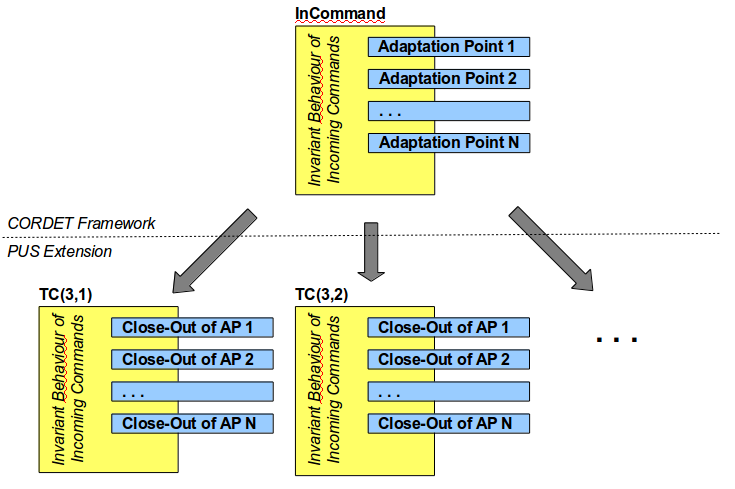
\includegraphics[scale=0.415,keepaspectratio=true]{InCmdAdaptation.png}
 \caption{Extension of InCommand Component}
 \label{fig:InCmdAdaptation}
\end{figure}

The components of the CORDET Framework are defined as models which comply with the FW Profile of [FW-SP]. By way of example, figure \ref{fig:CrFwInCommand} shows the model of the InCommand (the figure is taken from [CR-SP]). This consists of a state machine where some guards and actions are marked as "Adaptation Points". Concrete commands are defined by attaching a concrete behaviour to these actions and guards.

Thus, for each supported PUS command, the framework extension defines an extension of the InCommand component which closes all the InCommand adaptation points. Similarly, for each supported PUS report, it defines an extension of the OutComponent component which closes all the OutComponent adaptation points.

Table \ref{tab:listOfServices} and \ref{tab:listOfCmdRep} list the PUS services supoorted (either in full or in part) and the command and report components provided by the PUS Extension of the CORDET Framework to implement them. The first column in table \ref{tab:listOfCmdRep} gives the [type,sub-type] pair which identifies the command or report; the second column gives the name of the CORDET component which implements the command or report; the last column gives its PUS names as it is given in section 8 of [PS-SP]. 

\begin{figure}[H]
 \centering
 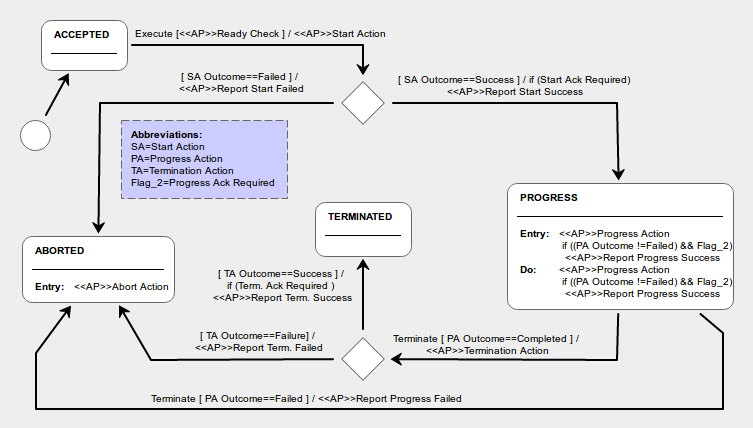
\includegraphics[scale=0.5,keepaspectratio=true]{CrFwInCommand.png}
 \caption{Model of InCommand Component}
 \label{fig:CrFwInCommand}
\end{figure}


%--------------------------------------------------------------------------------------
\subsection{Report and Command Adaptation Points}\label{sec:repCmdAP}
Tables \ref{tab:AP-OCM} and \ref{tab:AP-ICM} list the adaptation points of, respectively, the OutComponent component and the InCommand component. These adaptation points are defined by the CORDET Framework in [CR-SP]. The tables show how they are closed for the concrete commands and reports supported by the PUS Extension of the framework. In some cases, the adaptation point is closed in the same way for all framework reports/commands. In other cases, the close-out is report- or command-specific and is then described in the later sections of this document which define the individual PUS services. Thus, for instance, the close-out of the report-specific adaptation points for the service 1 reports can be found in section \ref{sec:serv1AP}. 

The following considerations apply to the data in table \ref{tab:AP-OCM} concerning OutComponents:

\begin{itemize}
\item The OutComponent components are created by the OutFactory and it can be assumed that they are created such that they can be successfully initialized and configured. Their initialization and configuration procedures (adaptation points OCM-1 to 4) can therefore be just dummies that do not perform any action. The same applies to the shutdown procedure (adaptation point OCM-5).
\item The adaptation point OCM-6 related to the execution procedure is already closed at CORDET Framework level because OutComponents have no execution procedure.
\item The adaptation points OCM-7 and 8 related to the setting of the report type and sub-type are closed in accordance with the discussion in section \ref{sec:repCmdAttr} by setting the CORDET types and sub-types equal to the PUS type and sub-type.
\item The adaptation points OCM-9 and OCM-10 to 12 related to the setting of the report discriminant, destination and parameters are closed for each individual report type in the following sections of this document.
\item The adaptation point OCM-10 related to the acknowledge level is only relevant to out-going commands and is therefore not applicable to the PUS reports defined in this document (which is only concerned with incoming commands).
\item The adaptation points OCM-13 to 16 related to the report checks and actions are closed for each specific report type in the following sections of this document.
\item The adaptation point OCM-17 related to the serialize operation is closed to create a packet layout which complies with the layout defined by the PUS in [PS-SP].
\item The adaptation point OCM-18 covers the response to a report having an invalid destination. By design, this situation should never arise and the adaptation point is closed with the generation of an error report.
\end{itemize}

The following considerations apply to the data in table \ref{tab:AP-ICM} concerning InCommands:

\begin{itemize}
\item The InCommand components are created by the InFactory but are then initialized and configured by the InLoader. Their initialization and configuration procedures (adaptation points ICM-1 to 4) are therefore implementation-specific. The same applies to the shutdown procedure (adaptation point ICM-5).
\item The adaptation point ICM-3 implements the acceptance check for the command. This verifies the correctness of the command length and CRC.
\item The adaptation point related to the execution procedure (ICM-6) is already closed at CORDET Framework level because InCommand do not have any execution procedure.
\item The adaptation points ICM-7 to 11 related to the command checks and actions are closed for each specific command type in the following sections of this document.
\item The adaptation points ICM-12 to 17 related to the generation of success and failure reports for the command are closed as part of the service 1 definition in section \ref{sec:serv1AP}.
\item The adaptation points ICM-18 and 19 related to the setting of the command type and sub-type are closed in accordance with the discussion in section \ref{sec:repCmdAttr} by setting the CORDET types and sub-types equal to the PUS type and sub-type.
\item The adaptation points ICM-20 and 21 related to the command discriminant and parameters are closed for each individual command type in the following sections of this document.
\end{itemize}

\begin{crAp}{OCM}{Adaptation Points for PUS Reports}
\end{crAp}

\newpage
\begin{crAp}{ICM}{Adaptation Points for PUS Commands}
\end{crAp}

%--------------------------------------------------------------------------------------
\subsection{Dependencies Between Services}\label{sec:dependencies}
A service S1 depends on another service S2 if the decision by an application to deploy service S1 requires the same application to also deploy service S2. The services defined in this document minimize this kind of dependencies. Table \ref{tab:dependencies} lists the service dependencies. These are limited to:

\begin{itemize}
\item Services 12 and 13 generate event reports and therefore need service 5
\end{itemize}

Note that, although dependencies between services are minimized, all services depend on the data pool because the data pool holds the variable and parameters which are used by the services. Hence, all applications instantiated from the CORDET Extension of the PUS Framework must deploy the data pool component of section \ref{sec:dp}.


\begin{pnptable}{|c|>{\raggedright\arraybackslash}p{5cm}|>{\raggedright\arraybackslash}p{3cm}|}{Service Dependencies}{tab:dependencies}{\textbf{N} & \textbf{Service Name} & \textbf{Dependencies}}
\texttt{1} & Request Verification Service & None \\
\hline
\texttt{3} & Housekeeping Service & None \\
\hline
\texttt{5} & Event Reporting Service & None \\
\hline
\texttt{12} & On-Board Monitoring Service & Requires Service 5 \\
\hline
\texttt{13} & Large Packet Transfer Service & Requires Service 5 \\
\hline
\texttt{17} & Test Service & None \\
\hline
\texttt{19} & Event Action Service & TBD \\
\hline
\end{pnptable}  


\newpage
%--------------------------------------------------------------------------------------
\subsection{Requirements}\label{sec:repCmdReq}
The requirements in table \ref{tab:Req-PCR} make the adaptation points defined in the previous two sections applicable to all command and report components provided by the framework extension.

\begin{crReq}{PCR}{Requirements for Framework Extension Commands and Reports}
\end{crReq}

\pnpcsvtable{|c|c|p{6cm}|}{List of Supported Services}{tab:listOfServices}{Type & Acron. & Name}{./GeneratedTables/PUSExtensionServices.csv}{\Type & \Name & \Description}

\newpage
\pnpcsvtable{|c|l|p{7cm}|}{List of Supported Commands/Reports}{tab:listOfCmdRep}{Type & CORDET Name & PUS Name}{./GeneratedTables/PUSExtensionServiceOverview.csv}{\Type & \Name & \Description}









%=============================================================================================
\section{Request Verification Service}\label{sec:serv1}
The service type of the Request Verification Service is 1. The PUS Extension of the CORDET Framework supports this service in full.

The Request Verification Service is implemented by nine reports which are issued  in response to notifications generated by a service provider application. The notifications cover different stages of the processing of an incoming command. More precisely:

\begin{itemize}
\item The report (1,10) is triggered in response to notifications of a routing failure for an incoming command (Routing and Reporting Sub-Service)
\item The report (1,1) and (1,2) are triggered in response to notifications of the failure or success of the acceptance of an incoming command (Acceptance and Reporting Sub-Service) 
\item The reports (1,3) to (1,8) are triggered in response to notifications of the failure or success of execution of an incoming command (Execution and Reporting Sub-Service)
\end{itemize}

The notifications listed above are generated by the CORDET Framework infrastructure. The operations which generate them are defined as adaptation points. The PUS Extension closes these adaptation points to generate the service 1 reports. 

An example may help clarify the mechanism through which the service 1 reports are generated. The InCommand state machine of the CORDET Framework defines the generic behaviour of incoming commands. Among other things, this state machine stipulates that, when the execution of an incoming command has been successfully completed, the Report-Termination-Successful Operation is called to notify other parts of the application that the command has successfully terminated. At the level of the CORDET Framework, this operation is defined as an adaptation point (because, at this level, it is not possible to define how and to whom the notification of successful completion should be distributed). At the level of the PUS Extension this adaptation point is closed by having the Report-Termination-Successful Operation generate a service 1 report of type (1,7).

The notifications generated by the CORDET Framework are generated in response to checks performed on incoming commands. However, the PUS stipulates that execution notifications may also be generated in response to checks performed on individual instructions embedded within a command. These notifications cannot be generated by the CORDET Framework which only handles abstract commands. These execution notifications are therefore generated by individual commands as part of their processing of their own instructions. An example may again help clarify this logic. The PUS command of type (3,5) carries several instructions each of which enables one housekeeping report. The processing of these instructions is done by the actions associated to the command itself and the generation of the instruction-level notifications is therefore done by these actions. Note that, as discussed in section \ref{sec:ComplianceToPus}, for instructions, only execution failures are reported.

By way of summary, table \ref{tab:sourcesNotif} lists the sources of all notifications which may trigger service 1 reports. For notifications which are issued by the CORDET Framework infrastructure, the rightmost column in the table identifies the corresponding adaptation point.



\begin{longtable}{|>{\raggedright\arraybackslash}p{2.1cm}|>{\raggedright\arraybackslash}p{9.8cm}|c|}
\caption{Sources of Routing, Acceptance and Execution Notifications}\label{tab:sourcesNotif} \\
\hline
\rowcolor{light-gray}
\textbf{Notification} & \textbf{Source} & \textbf{AP} \\
\hline\hline
\endfirsthead
\rowcolor{light-gray}
\textbf{Notification} & \textbf{Source} & \textbf{AP} \\
\hline\hline
\endhead
Routing Failure Notification & This notification is issued by the \textit{Report Packet Destination Invalid Operation} which is called by the InLoader Execution Procedure when an application has received a command or report with a destination which is neither the application itself nor some other known application. & ILD-12 \\
\hline
Acceptance Failure Notification & This notification is issued by the \textit{Report Acceptance Failure Operation} which is called by the InLoader Load Command/Report Procedure when: (a) an incoming command has failed its acceptance check, or (b) the InCommand component could not be created either to a lack or resources or to the triplet [type,sub-type,discriminant] being illegal, or (c) the InCommand component could not be loaded into its InManager due to the InManager Pending Command/Report List (PCRL) being full. & ILD-14 \\
\hline
Acceptance Success Notification & This notification is issued by the \textit{Report Acceptance Success Operation} which is called by the InLoader Load Command/Report Procedure when an incoming command has passed its Acceptance Check and that command has requested acknowledgement of successful acceptance. & ILD-15 \\
\hline
Execution Start Success Notification &  This notification is issued by the \textit{Report Start Successful for InCommand Operation} which is called by the InCommand State Machine when the Start Action of an incoming command has a 'success' outcome and that command has requested acknowledgement of successful start of execution. & ICM-13 \\
\hline 
Execution Start Failure Notification &  This notification is issued by the \textit{Report Start Failed for InCommand Operation} which is called by the InCommand State Machine when the Start Action of an incoming command has a 'failure' outcome. The same operation may also be called by the implementation of the Start Action of a command to report the failure of an instruction within the command. & ICM-12 \\
\hline
Execution Progress Success Notification &  This notification is issued by the \textit{Report Progress Successful for InCommand Operation} which is called by the InCommand State Machine when the Progress Action of an incoming command has a 'success' outcome and that command has requested acknowledgement of successful progress of execution. & ICM-15 \\
\hline
Execution Progress Failure Notification &  This notification is issued by the \textit{Report Progress Failed for InCommand Operation} which is called by the InCommand State Machine when the Progress Action of an incoming command has a 'failure' outcome. The same operation may also be called by the implementation of the Progress Action of a command to report the failure of the execution step of an instruction within the command. & ICM-14 \\
\hline 
Execution Termination Success Notification &  This notification is issued by the  \textit{Report Termination Successful for InCommand Operation} which is called by the InCommand State Machine when the Termination Action of an incoming command has a 'success' outcome and that command has requested acknowledgement of successful termination of execution. & ICM-17 \\
\hline
Execution Termination Failure Notification &  This notification is issued by the \textit{Report Termination Failed for InCommand Operation} which is called by the InCommand State Machine when the Termination Action of an incoming command has a 'failure' outcome. & ICM-16 \\
\hline
\end{longtable} 

The framework extension closes the adaptation points in table \ref{tab:sourcesNotif} with behaviour which generates the service 1 verification reports. The first row in the table corresponds to a situation where a packet cannot be re-routed, which if the packet contains a command, is the situation where the PUS prescribes that a (1,10) report should be generated. The other rows correspond to situations where an incoming command has either failed or passed one of its processing checks and they are therefore closed with the generation of the service 1 reports (1,1) to (1,8). 

The close-out behaviour for the adaptation points is defined in table \ref{tab:AP-S1}. It consists of running a procedure which creates the service 1 report, configures it, and then loads it into the OutLoader. The report is created by calling the \texttt{Make} operation of the OutFactory. This may fail if the OutFactory has run out of resources for new reports. In that case, error report OUTFACTORY\_FAIL is generated. Procedures which report failures also update the relevant observables (see section \ref{sec:serv1Obs}).

The failure code of failure reports in service 1 is treated as a discriminant. This allows applications to selectively disable certain failure reports by using the enable mechanism of the OutRegistry component of the CORDET Framework. It is recalled that this mechanism allows the OutRegistry to be configured to disable out-going reports by 'kind' where the kind of a report is defined by the triplet: [type, sub-type, discriminant]. 


%---------------------------------------------------------------------------------
\subsection{Service 1 Report and Command Definition}\label{sec:serv1RepDef}
There are no commands in service 1. The service is only implemented by reports. In the CORDET Framework an out-going report is encapsulated in an OutComponent component. The framework extension offers, for each service 1 report, an component to encapsulate it. These components are implemented as extension of the OutComponent component. They are therefore defined by the way they close the adaptation points of the OutComponent. The tables in this section list the OutComponent adaptation points and show how they are closed for the service 1 components.

The PUS defines the content of the service 1 reports in section 8.1 of AD-3. The 'success' reports carry the packet identifier of the command being verified. The 'failure' reports carry, in addition to the packet identifier, a failure code and an undefined set of failure-related data. The framework extension restricts this flexibility by stipulating that the failure-related data consist of: 

\begin{itemize}
\item For all failure reports: the triplet [type,sub-type,discriminant] for the command being verified
\item For all failure reports but (1,10) reports: the \textit{Verification Failure Data} as a single data item which contains command-specific information about the failure 
\item For (1,10) reports only: the destination of the command which failed its routing check
\item For (1,5) reports only: the identifier of the step which failed its progress check
\end{itemize}

The Verification Failure Code and the Verification Failure Data are stored in data pool items \texttt{verFailCode} and \texttt{verFailData}. The purpose of \texttt{verFailData} is to provide additional information about the nature of the failure being reported by the failure report. This data item has a fixed size but its syntactical type is command-specific. Its value is set by the entity which performs the verification check. If no failure data are defined for a given verification check, then the value of \texttt{verFailData} is "don't care". 

To illustrate, consider the case of a command (3,5) which enables a housekeeping report. This command carries the Structure Identifier (SID) of the report to be enabled. The Start Action of this command checks the legality of the SID (see section \ref{sec:serv3}). If the SID is found to be illegal, the command is rejected with a (1,4) report and the illegal SID value is used as Verification Failure Data. The Start Action of the (1,4) command loads the illegal SID into data pool item \texttt{verFailData} and the Command Verification Failure Procedure which creates the (1,4) report takes the Verification Failure Data from \texttt{verFailData}.

The Verification Failure Codes which are supported by the PUS Extension are listed in appendix \ref{sec:reqVerFailCodes}. These failure codes cover the failure conditions for the commands defined by the PUS Extension. For each failure code, the associated verification failure data is also defined. Applications should extend the table in appendix \ref{sec:reqVerFailCodes} with the failure codes for their own commands. 

The tables in this section formally specify the service 1 components by specifying how the actions, checks and attributes of a generic out-going report are specialized for service 1 (see section \ref{sec:defPusRepCmd}). The following remarks apply: 

\begin{itemize}
\item Service 1 reports retrieve their enable status from the OutRegistry.
\item Service 1 reports are generated as soon as the condition which triggered them occur and hence their ready check always returns 'ready'
\item Service 1 reports are 'one-off' reports and hence their repeat check always returns 'no repeat'
\end{itemize}

With reference to the first bullet, it is recalled that the OutRegistry component of the CORDET Framework stores the enable status of out-going reports as a function of the report's type, sub-type and discriminant. By default, all out-going reports are enabled. Users who wish to disable a specific service 1 sub-type can do so by setting its status to 'disabled' in the OutRegistry. This is a run-time operation which would typically be done as part of an application's initialization.

\printOutCmpVerSuccAccRepSpec{|c|p{10cm}|}
\printOutCmpVerFailedAccRepSpec{|c|p{10cm}|}
\newpage
\printOutCmpVerSuccStartRepSpec{|c|p{10cm}|}
\printOutCmpVerFailedStartRepSpec{|c|p{10cm}|}
\newpage
\printOutCmpVerSuccPrgrRepSpec{|c|p{10cm}|}
\printOutCmpVerFailedPrgrRepSpec{|c|p{10cm}|}
\newpage
\printOutCmpVerSuccTermRepSpec{|c|p{10cm}|}
\printOutCmpVerFailedTermRepSpec{|c|p{10cm}|}
\newpage
\printOutCmpVerFailedRoutingRepSpec{|c|p{10cm}|}


%---------------------------------------------------------------------------------
\subsection{Service 1 Observables}\label{sec:serv1Obs}
Service 1 maintains and makes available in the data pool various information related to the generation of the failure reports. No information related to the generation of the success reports is maintained because these reports are optional and the conditions under which they are generated depend on the setting of the verification acknowledge flags which are under external control (they are set by the user of a service). Table \ref{tab:Obs-S1} lists the data pool data items which are maintained by service 1.

\pnpcsvtable[filter equal={\Domain}{Ver}]{|p{4cm}|>{\raggedright\arraybackslash}p{9cm}|}{Observables for Verification Service}{tab:Obs-S1}{Name & Description}{./GeneratedTables/Datapool.csv}{\texttt{\Name} & \ShortDesc}


%---------------------------------------------------------------------------------
\subsection{Service 1 Adaptation Points}\label{sec:serv1AP}
Table \ref{tab:AP-S1} lists the CORDET Framework adaptation points which are closed or overridden by the request verification service. 

\begin{crAp}{S1}{Adaptation Points for Service 1 (Request Verification)}
\end{crAp}


%---------------------------------------------------------------------------------
\subsection{Service 1 Requirements}
The table in this section lists requirements for the request verification service.

\begin{crReq}{S1}{Requirements for Service 1 (Request Verification)}
\end{crReq}


\newpage
\begin{figure}[H]
 \centering
 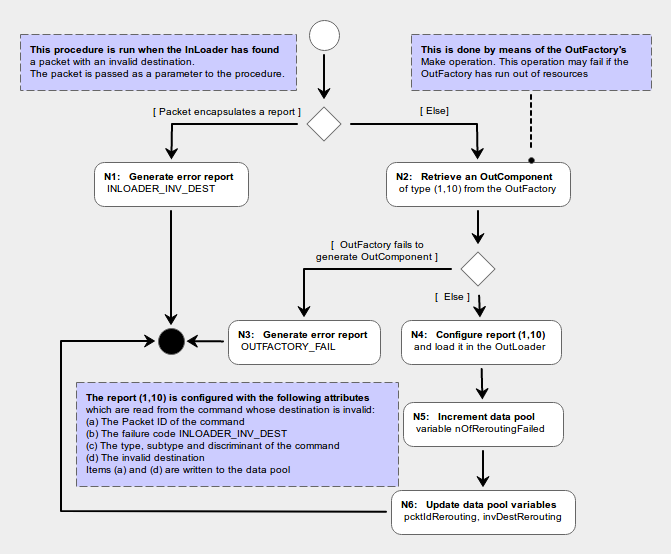
\includegraphics[scale=0.415,keepaspectratio=true]{CrPsPcktReroutingFail.png}
 \caption{Packet Rerouting Failure Procedure}
 \label{fig:PcktReroutingFail}
\end{figure}

\begin{figure}[htbp]
 \centering
 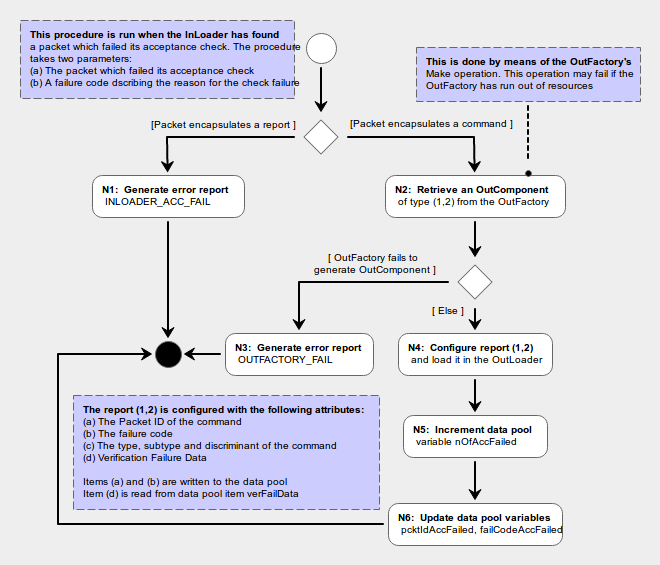
\includegraphics[scale=0.414,keepaspectratio=true]{CrPsPcktAccFail.png}
 \caption{Packet Acceptance Failure Procedure}
 \label{fig:PcktAccFail}
\end{figure}

\begin{figure}[htbp]
 \centering
 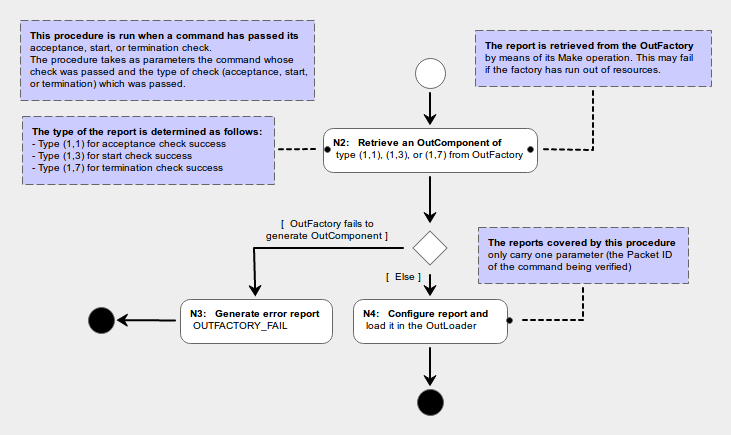
\includegraphics[scale=0.415,keepaspectratio=true]{CrPsCmdVerSucc.png}
 \caption{Command Verification Success Procedure}
 \label{fig:CmdVerSucc}
\end{figure}

\begin{figure}[htbp]
 \centering
 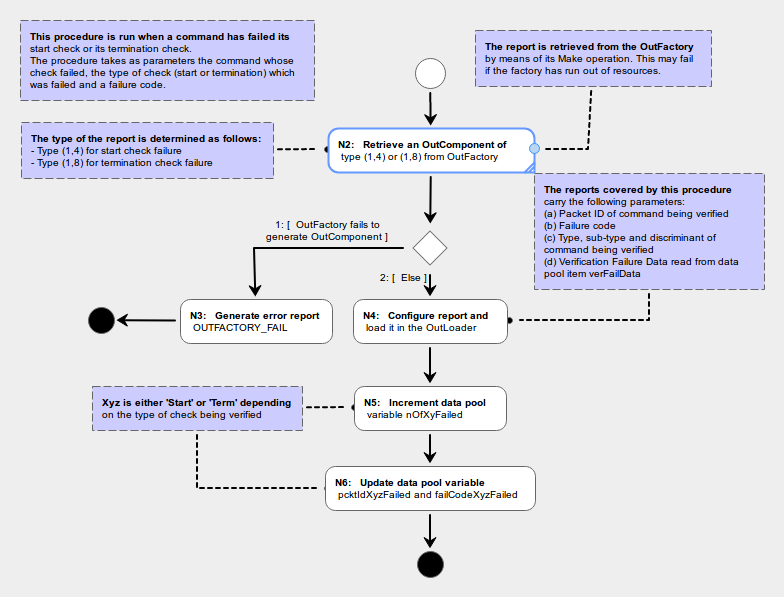
\includegraphics[scale=0.415,keepaspectratio=true]{CrPsCmdVerFail.png}
 \caption{Command Verification Failure Procedure}
 \label{fig:CmdVerFail}
\end{figure}

\begin{figure}[htbp]
 \centering
 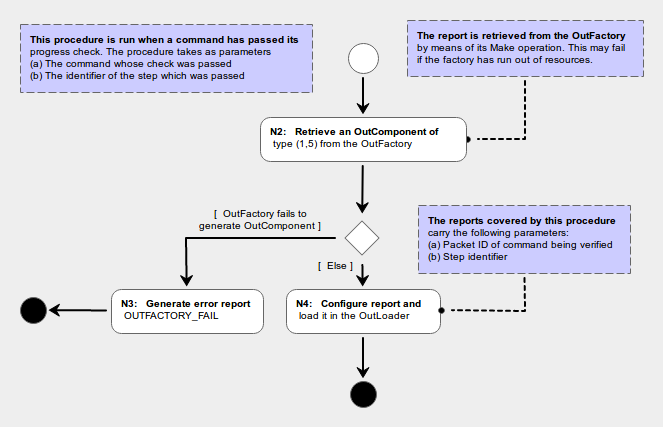
\includegraphics[scale=0.415,keepaspectratio=true]{CrPsCmdPrgrSucc.png}
 \caption{Command Progress Success Procedure}
 \label{fig:CmdPrgrSucc}
\end{figure}

\begin{figure}[H]
 \centering
 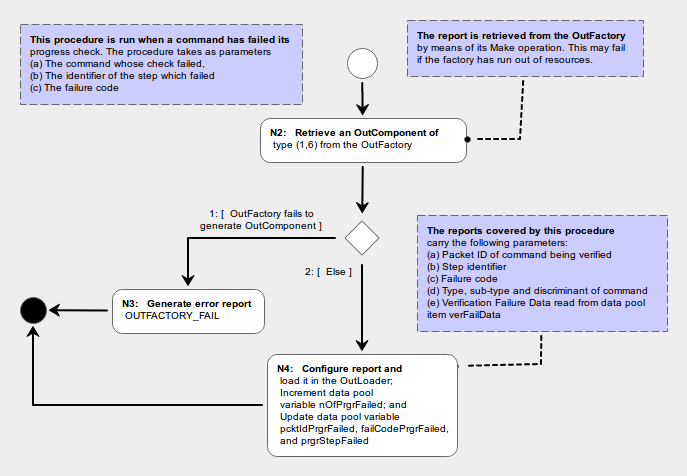
\includegraphics[scale=0.415,keepaspectratio=true]{CrPsCmdPrgrFail.png}
 \caption{Command Progress Failure Procedure}
 \label{fig:CmdPrgrFail}
\end{figure}

%=============================================================================================
\section{Housekeeping Service}\label{sec:serv3}
The service type of the Housekeeping Service is 3. The PUS Extension of the CORDET Framework supports this service only in part.

The housekeeping service provides the capability to create, delete and control housekeeping and diagnostic reports. The service 3 commands and reports in the PUS are duplicated being defined once for housekeeping reports and once for diagnostic reports. The PUS framework supports both sets of commands and reports but does not otherwise make any distinction between housekeeping and diagnostic reports. It is essentially up to the user to decide which service 3 reports should be treated as 'housekeeping reports' and which ones should instead be treated as 'diagnostic reports'.

A housekeeping/diagnostic report carries the values of a set of data pool items\footnote{The PUS uses the term 'parameter' to designate the data pool items whose values are carried by the housekeeping and diagnostic reports.}. Any data pool item may be included in a housekeeping/diagnostic report. 

At any given time, an application generates several kinds of housekeeping/diagnostic reports which differ for the set of data items they hold and for the frequency with which they are generated. The housekeeping/diagnostic reports use the discriminant attribute to manage this variability. Thus, two different kinds of housekeeping/diagnostic reports are distinguished by different values of discriminant attribute. In keeping with the PUS convention, the discriminant attribute of a housekeeping/diagnostic report is called \textit{Structure Identifier} or SID. The SID must be a positive integer in the range: 1..HK\_MAX\_SID.

Since no distinction is made between housekeeping and diagnostic reports, the SID must be unique within the set of all housekeeping/diagnostic reports (i.e. it is not possible for a housekeeping report and a diagnostic report to have the same SID).

Housekeeping/diagnostic reports may be generated periodically or in "one-shot" mode. For periodic reports, the \textit{Collection Period} is the period with which the report is generated. The Collection Period is expressed as an integer multiple of a minimum period HK\_COLLECT\_PER which is an application constant. A value of zero for the Collection Period indicates that the report must be generated in "one-shot" mode.

A data item in a housekeeping/diagnostic report is either \textit{simply commutated} or \textit{super-commutated}. The value of a simply-commutated data item appears only once in the housekeeping/diagnostic report and it represents the value of the data item at the time the report is generated.

The value of a super-commutated data item instead appears multiple times within a housekeeping/diagnostic report. Super-commutated data items in a report are divided into \textit{groups}. To each group, a \textit{sample repetition number} N is associated: a report carries N values of the data items in the super-commutated group. These N values have been generated by sampling the data items at N distinct points in time within the collection period. The PUS stipulates that the N collection points must be equally spaced within the collection interval but this constraint is not enforced by the framework (but may be enforced at application-level). 

The PUS also stipulates that, within a housekeeping/diagnostic report definition, each data item appears only once, either as a simply commutated parameter or as a super-commutated parameter. This restriction is not enforced by the framework.

%-------------------------------------------------------------------------------------
\subsection{Report Definition List (RDL)}\label{sec:serv3RDL}
The Reporting Definition List or RDL is a data structure which holds the current configuration of the housekeeping/diagnostic reports. The content of the RDL is updated by the service 3 commands and, on request, it may be reported by service 3 reports.

The RDL holds HK\_N\_REP\_DEF \textit{Report Definitions}. The value of HK\_N\_REP\_DEF is an application constant. It represents the maximum number of housekeeping/diagnostic reports which may be defined at a given time. 

Each Report Definition defines one housekeeping/diagnostic report in terms of the fields listed in table \ref{tab:repDefDataStruct}. Rows 6 to 9 determine the content of the report. The data items in a housekeeping/diagnostic report are arranged as a sequence of data item values according to the layout specified in clause 6.3.3.3 of [PS-SP]. The total number of reported data items is: (\texttt{nSimple}+\texttt{nRep[1]}+ .. +\texttt{nRep[nGroup]}), of which the first \texttt{nSimple} are simply-commutated whereas the others are split into \texttt{nGroup} groups of super-commutated data items. For each data item in the i-th group, \texttt{rep[i]} values are reported which have been collected at \texttt{rep[i]} times within the collection interval. The total number of data item values in a report therefore is: (\texttt{nSimple}+\texttt{nRep[1]*rep[1]}+ .. +\texttt{nRep[nGroup]*rep[nGroup]})

The parameters HK\_MAX\_* are application constants. Applications which do not need super-commutated data can set HK\_MAX\_N\_GR to zero.

The sampling buffer mentioned in the last row in table \ref{tab:repDefDataStruct} is discussed in the next section.

Several service 3 commands operate on a set of RDL entries (e.g. command (3,3) requests that a list of SIDs be deleted from the RDL). In such cases, it is useful to "mark" an entry in the RDL. For this purpose, flag \texttt{isMarked} has been introduced in table \ref{tab:repDefDataStruct}.


\begin{pnptable}{|l|p{5cm}|>{\raggedright\arraybackslash}p{6cm}|}{Fields in Report Definition Data Structure}{tab:repDefDataStruct}{\textbf{Field Name} & \textbf{Description} & \textbf{Constraint}}
\texttt{sid} & Structure identifier (SID) & Integer in range: 1..HK\_MAX\_SID \\
\hline
\texttt{period} & Collection period in units of HK\_COLLECT\_PER & Positive integer (periodic reports) or zero (one-shot reports) \\
\hline
\texttt{cycleCnt} & Cycle counter (see definition of service 3 reports and commands) & Integer in the range: 0..(\texttt{period}-1) \\
\hline
\texttt{isEnabled} & True if the report is enabled & None  \\
\hline
\texttt{dest} & The identifier of the application to which the report is sent & None \\
\hline
\texttt{nSimple} & Number of simply-commutated data items in the report & Integer in range: 1..HK\_MAX\_N\_SIMPLE \\
\hline
\texttt{lstSampleRep} & List of super commutated sample repetition numbers (\texttt{rep[1]} .. \texttt{rep[nGroup]}) & The number of groups is in the range: 0..HK\_MAX\_N\_GR and each repetition number is in the range: 1..HK\_MAX\_REP \\
\hline
\texttt{lstNSampRep} & List of numbers (\texttt{nRep[1]} .. \texttt{nRep[nGroup]}) of data items in each super-commutated group & Each \texttt{nRep[i]} is in range: 1..HK\_MAX\_N\_REP \\
\hline
\texttt{lstId} & List of identifiers of data items in the report & Not more than HK\_MAX\_N\_ITEMS data items and each identifier is in range: 1..HK\_MAX\_ID \\
\hline
\texttt{sampleBufId} & The identifier of the sampling buffer holding the super-commutated data item values & An integer in the range: 1..HK\_N\_SAMP\_BUF \\
\hline
\texttt{isMarked} & Marker flag & Boolean flag \\
\hline
\end{pnptable}  


%-------------------------------------------------------------------------------------
\subsection{Management of Super-Commutated Data Items}\label{sec:serv3SupCommDataItems}
The housekeeping service is responsible for collecting the values of the data items in housekeeping/diagnostic packets. For simply-commutated data items, the values are collected directly from the data pool. For super-commutated data items, the values are collected from a \textit{Sampling Buffer}. Each sampling buffer holds the values of the super-commutated data items for a given housekeeping/diagnostic report.

The super-commutated data items in a report are arranged in \texttt{nGroup} groups. The i-th group covers \texttt{nRep[i]} items which are sampled \texttt{nRep[i]} times within a collection period. Hence, in each collection period, the i-th group contributes: \texttt{nRep[i]*rep[i]} data item values. The sampling buffer for a given housekeeping/diagnostic report must be large enough to hold the data item values collected in one collection period for all super-commutated groups in that report.

The number of sampling buffers is HK\_N\_SAMP\_BUF. The value of HK\_N\_SAMP\_BUF is an application constant. It represents the maximum number of housekeeping/diagnostic reports with super-commutated data items which may be defined at a given time. This may be smaller than the maximum number HK\_N\_REP\_DEF of housekeeping/diagnostic reports. Thus, for instance, an application might stipulate that there may be up to 10 housekeeping/diagnostic reports but only two of these may contain super-commutated data items. This application would set HK\_N\_REP\_DEF to 10 and  HK\_N\_SAMP\_BUF to 2.

The association between housekeeping/diagnostic report and its sampling buffer is done dynamically: if a report has super-commutated data items, the last field in its report definition contains a pointer to its sampling buffer (see table \ref{tab:repDefDataStruct}).

The periodic collection of the values of the simply-commutated data items is done by the components hkRep which encapsulate a housekeeping/diagnostic report (see section \ref{sec:serv3RepCmdDef}). These components are executed once per collection interval. They therefore cannot collect the values of the super-commutated data items which are sampled several times per collection period. Responsibility for the collection of the values of the super-commutated data items rests with the application instantiated from the framework. 

The framework offers the following functions to manipulate a sampling buffer:

\begin{itemize}
\item \textit{Sampling Buffer Configuration Function} to configure a sampling buffer as a function of the number of groups, the number of data items in each group and the repetition number for each group.
\item Sampling Buffer Setter Function to load the i-th value of the j-th data item in the k-th group in the sampling buffer.
\item Sampling Buffer Getter Function to retrieve the i-th value of the j-th data item in the k-th group in the sampling buffer.
\end{itemize}

The Configuration Function is used when a housekeeping/diagnostic report which contains super-commutated data items is created (either at application initialization time for a pre-defined report or in response to a (3,1)/(3,2) command for a dynamically defined report). The Setter Function is used by the application to load the super-commutated values in the sampling buffer. The Getter Function is used in the Update Action of the (3,25) and (3,26) reports to update the content of a housekeeping/diagnostic report. 

%-------------------------------------------------------------------------------------
\subsection{Debug Variables}\label{sec:debugVar}
Service 3 offers visibility over the internal state of the IFSW by allowing periodic or sporadic access to the data items in the data pool. The data items in the data pool are defined at design time and should cover all application functions. For situations where additional visibility is required (e.g. in case of debugging during AIT activities), the framework the concept of \textit{debug variables} is introduced. A debug variable is a variable of 4 bytes of length whose address in RAM is a data pool parameter. More precisely, a total of N\_DEBUG\_VAR debug variables are defined which are encapsulated in data pool variables \texttt{debugVar\_x} where x ranges from 1 to HK\_N\_DEBUG\_VAR. Additionally, data pool parameters \texttt{debugVarAddr\_x} are defined to hold the address of \texttt{debugVar\_x}. The Execution Procedure of the data pool (see section \ref{sec:dpBehaviour}) loads the values of the memory locations pointed at by the elements of \texttt{debugVarAddr} into the elements of \texttt{debugVar}.  

In order to illustrate the use of the debug variables, consider a situation where the user wishes to have read access to two memory locations holding two integers: 

\begin{enumerate}
\item The user loads the addresses of the desired locations into the first two elements of \texttt{debugVarAddr}
\item The user uses command (3,1) or (3,2) to define a new housekeeping report packet holding \texttt{debugVar\_1} and \texttt{debugVar\_2} 
\item The users uses command (3,6) or (3,7) to enable the newly defined housekeeping packet and receives the values of \texttt{debugVar\_1} and \texttt{debugVar\_2} .
\end{enumerate}


%-------------------------------------------------------------------------------------
\subsection{Service 3 Report and Command Definition}\label{sec:serv3RepCmdDef}
The tables in this section formally specify the service 3 commands and reports by specifying how the actions, checks and attributes of generic out-going commands and reports are specialized for service 3 (see section \ref{sec:defPusRepCmd}). The following remarks apply:

\begin{itemize}
\item In the PUS, service 3 commands and reports appear twice: once for housekeeping reports and once for diagnostic reports. The PUS Extension of the CORDET Framework does not distinguish between housekeeping and diagnostic reports/commands and therefore each CORDET report/command component implements two PUS reports/commands.
\item Several commands in this service (e.g. the commands to delete a housekeeping/diagnostic report definition) carry multiple instructions which are executed independently of each other. In keeping with the general strategy outlined in section \ref{sec:ComplianceToPus}, their start action evaluates the instructions one by one and, in case of invalidity, it generates a (1,4) report for each individual instruction.
\item The (3,9) and (3,27) commands carry a sequence of SIDs. The command's Start Action removes invalid SIDs. The valid SIDs are then processed by the command's Progress Action. Each SID is processed in a progress step. In keeping with the strategy of section \ref{sec:ComplianceToPus}, only step failures are reported through service 1 reports. The command is deemed to have completed successfully if at least one SID has been successfully processed. 
\item For the housekeeping/diagnostic reports (3,25) and (3,26), two components are provided of which one is used when the reports are generated on a periodic basis and the other is used when the reports are generated in óne-shot' mode in response to a (3,27) or (3,28) command.
\end{itemize}

\printInCmdHkCreHkCmdSpec{|c|p{10cm}|}
\printInCmdHkCreDiagCmdSpec{|c|p{10cm}|}
\newpage
\printInCmdHkDelHkCmdSpec{|c|p{10cm}|}
\printInCmdHkDelDiagCmdSpec{|c|p{10cm}|}
\newpage
\printInCmdHkEnbHkCmdSpec{|c|p{10cm}|}
\printInCmdHkDisHkCmdSpec{|c|p{10cm}|}
\newpage
\printInCmdHkEnbDiagCmdSpec{|c|p{10cm}|}
\printInCmdHkDisDiagCmdSpec{|c|p{10cm}|}
\newpage
\printInCmdHkRepStructHkCmdSpec{|c|p{10cm}|}
\printOutCmpHkRepStructHkRepSpec{|c|p{10cm}|}
\newpage
\printInCmdHkRepStructDiagCmdSpec{|c|p{10cm}|}
\printOutCmpHkRepStructDiagRepSpec{|c|p{10cm}|}
\newpage
\printOutCmpHkRepSpec{|c|p{10cm}|}
\printOutCmpHkDiagRepSpec{|c|p{10cm}|}
\newpage
\printInCmdHkOneShotHkCmdSpec{|c|p{10cm}|}

%---------------------------------------------------------------------------------
\subsection{Service 3 Constants}\label{sec:serv3Const}
The service 3 constants are listed in table \ref{tab:Const-S3}.

\pnpcsvtable[filter equal={\Domain}{Hk}]{|p{3cm}|>{\raggedright\arraybackslash}p{9.5cm}|}{Constants for Housekeeping Service}{tab:Const-S3}{Name & Description}{./GeneratedTables/Constants.csv}{\texttt{\Name} & \Desc}


%---------------------------------------------------------------------------------
\subsection{Service 3 Observables and Parameters}\label{sec:serv3Obs}
The service 3 internal state is defined by the content of the Report Definition List (RDL). Most of its content is visible through reports (3,10) and (3,11). The observables defined by the framework only cover the non-visible part of the RDL state. 

Similarly, the service 3 configuration is defined by the content of the Report Definition List (RDL). This configuration is mostly controlled through commands (3,1)/(3,2) and (3,5)/(3,7) and is partially observable through reports (3,10) and (3,11). The service 3 configuration parameters which are either not controllable through service 3 commands and/or not observable through service 3 reports are defined as data pool parameters. 

The observables and the parameters for service 3 are listed in table \ref{tab:Obs-S3}.

\pnpcsvtable[filter equal={\Domain}{Hk}]{|p{3cm}|l|>{\raggedright\arraybackslash}p{6.0cm}|c|}{Observables and Parameters for Housekeeping Service}{tab:Obs-S3}{Name & Kind & Description & Multiplicity}{./GeneratedTables/Datapool.csv}{\texttt{\Name} & \Kind & \ShortDesc & \Multiplicity}

%---------------------------------------------------------------------------------
\subsection{Service 3 Requirements}
The table in this section lists requirements for the test service.

\begin{crReq}{S3}{Requirements for Service 3 (Housekeeping Service)}
\end{crReq}

\begin{figure}[H]
 \centering
 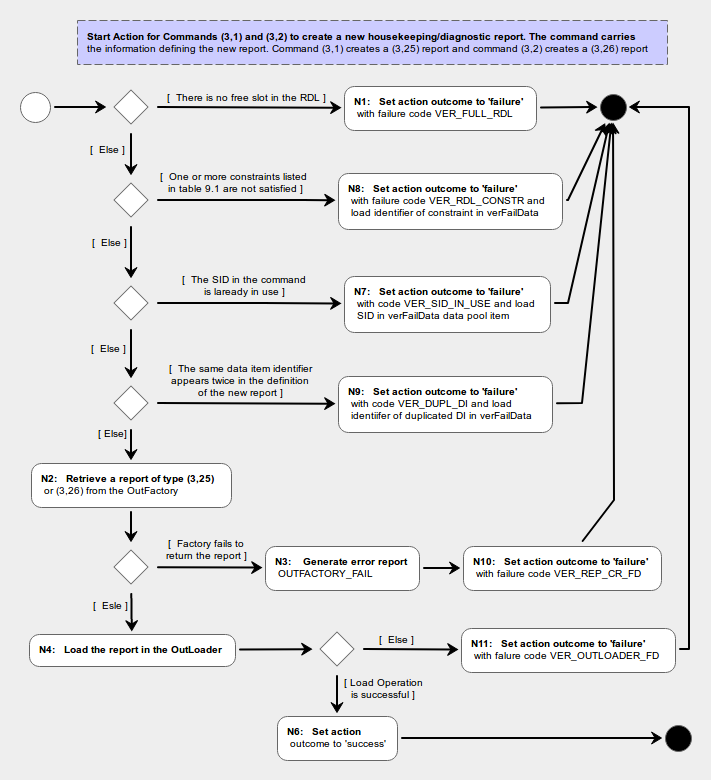
\includegraphics[scale=0.55,keepaspectratio=true]{CrPsCmd3s1Start.png}
 \caption{Start Action of Command to Create a Service 3 Packet}
 \label{fig:Cmd3s1Start}
\end{figure}

\begin{figure}[H]
 \centering
 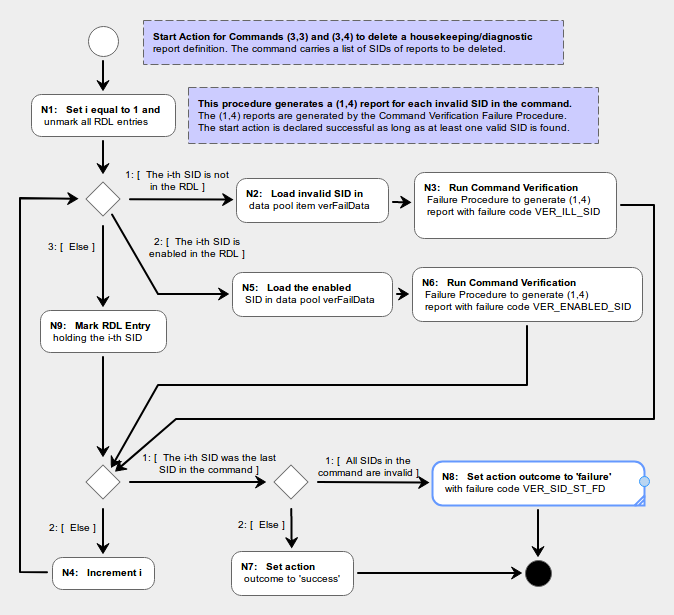
\includegraphics[scale=0.55,keepaspectratio=true]{CrPsCmd3s3Start.png}
 \caption{Start Action of Command to Delete a Service 3 Packet}
 \label{fig:Cmd3s3Start}
\end{figure}

\begin{figure}[H]
 \centering
 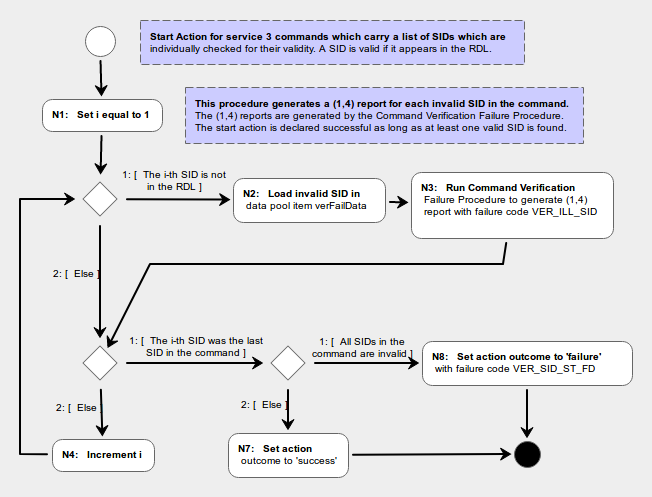
\includegraphics[scale=0.55,keepaspectratio=true]{CrPsCmd3SidStart.png}
 \caption{Start Action of Multi-SID Commands}
 \label{fig:Cmd3SidStart}
\end{figure}

\begin{figure}[H]
 \centering
 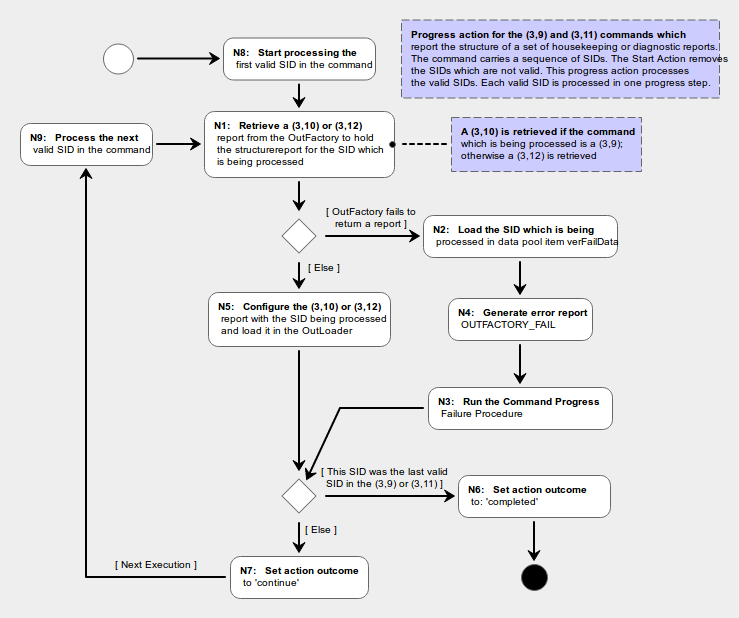
\includegraphics[scale=0.55,keepaspectratio=true]{CrPsCmd3s9Prgr.png}
 \caption{Progress Action of Command to Report the Structure of a Service 3 Packet}
 \label{fig:Cmd3s9Prgr}
\end{figure}

\begin{figure}[H]
 \centering
 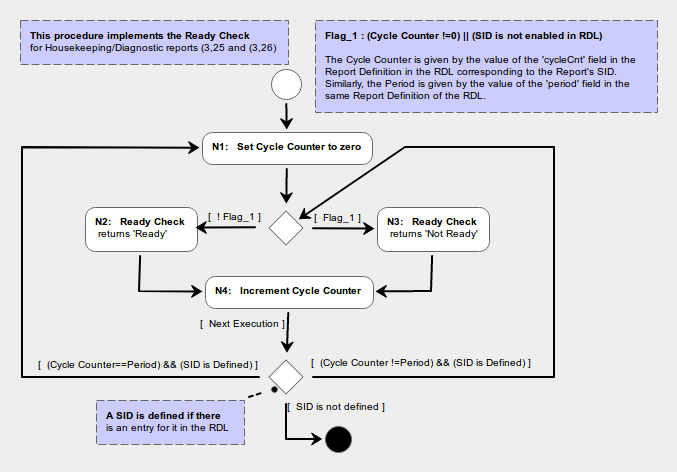
\includegraphics[scale=0.55,keepaspectratio=true]{CrPsRep3s25Ready.png}
 \caption{Ready Check of Report HkRep}
 \label{fig:Rep3s25Ready}
\end{figure}


%=============================================================================================
\section{Event Reporting Service}\label{sec:serv5}
The service type of the Event Reporting Service is 5. The PUS Extension of the CORDET Framework supports this service in full.

The event reporting service provides the capability to report event-like occurrences and to control the generation of event reports by enabling and disabling individual event identifiers.

The PUS recognizes four levels of event reports and associates to each level a service sub-type. Thus, for instance, all event reports of level 1 are carried by reports of type (5,1) and all event reports of level 2 are carried by event reports of type (5,2). 

All event reports have the same behaviour irrespective of their level. The PUS Extension of the CORDET Framework one component for each event reporting level.

Event reports may carry data. The Event Identifier (EID) determines the format of the data associated to an event report. The PUS Extension accordingly treats the event identifier as a discriminant. The range of discriminants and the data associated to each discriminant are adaptation points which must be defined at application level. Some event identifiers are pre-defined at framework level. They are listed in appendix \ref{sec:preDefEvtRep}.

Applications use event reports as follows:

\begin{itemize}
\item When an application encounters a situation which should trigger the generation of an event report, it retrieves an event component from the OutFactory. This component will encapsulate the event report. The event level and the event identifier are specified when the event component is retrieved from the factory because the 'make' function of the OutFactory takes as an argument the type and the sub-type of the event report.
\item The application loads the event component in the OutLoader. From this point onward, the event report is processed by the CORDET Framework infrastructure:
	\begin{itemize}
	\item If the identifier of the event is enabled, then the event report will eventually be sent to its destination;
	\item If the identifier of the event is not enabled, then the event report will be discarded.
	\end{itemize}
\end{itemize}

Note that the configuration of the event reports must be done by the application (as opposed to being delegated to the Update Action of the component which implements the event report). This ensures that the event report configuration reflects the state of the system at the time the event report is created (as opposed to the time when the event report is sent out).  

Event identifiers can be enabled and disabled. The PUS Extension uses the report enable mechanism of the OutRegistry component to manage the enable status of event reports. This implies that, by default, all event identifiers are enabled. If an application needs some event identifiers to be disabled by default, it must disable them during the application initialization phase (adaptation point P-S5-3).

In accordance with clause 6.5.4b of reference [PS-SP], all event reports have the same destination and this destination must be statically defined. The destination is accordingly treated as a configuration parameter for the PUS Extension of the CORDET Framework. The event destination is set by the Update Action of the event report.

%-------------------------------------------------------------------------------------
\subsection{Service 5 Report and Command Definition}\label{sec:serv5RepCmdDef}
The tables in this section formally specify the service 5 commands and reports by specifying how the actions, checks and attributes of generic out-going commands and reports are specialized for service 5 (see section \ref{sec:defPusRepCmd}). The following remarks apply:

\begin{itemize}
\item The update of observables which are related to the occurrence of an event is done by the Enable Check of component EvtRep. This is appropriate because this action is executed every time an application creates an event report. The update of observables which are related to the generation of report is done by the Update Action of component EvtRep. This is appropriate because this action is only executed when an event report is actually issued by an application.
\item Service 5 reports are generated as soon as the condition which triggered them occur and hence their ready check always returns 'ready'
\item Service 5 reports are 'one-off' reports and hence their repeat check always returns 'no repeat'
\end{itemize}

\newpage
\printOutCmpEvtRepaSpec{|c|p{10cm}|}
\printOutCmpEvtRepbSpec{|c|p{10cm}|}
\newpage
\printOutCmpEvtRepcSpec{|c|p{10cm}|}
\printOutCmpEvtRepdSpec{|c|p{10cm}|}
\newpage
\printInCmdEvtEnbCmdSpec{|c|p{10cm}|}
\printInCmdEvtDisCmdSpec{|c|p{10cm}|}
\newpage
\printInCmdEvtRepDisCmdSpec{|c|p{10cm}|}
\printOutCmpEvtDisRepSpec{|c|p{10cm}|}


%---------------------------------------------------------------------------------
\newpage
\subsection{Service 5 Constants}\label{sec:serv5Const}
The service 5 constants are listed in table \ref{tab:Const-S5}. 

\pnpcsvtable[filter equal={\Domain}{Evt}]{|p{3cm}|>{\raggedright\arraybackslash}p{9.5cm}|}{Constants for Event Reporting Service}{tab:Const-S5}{Name & Description}{./GeneratedTables/Constants.csv}{\texttt{\Name} & \Desc}


%---------------------------------------------------------------------------------
\subsection{Service 5 Observables}\label{sec:serv5Obs}
The service 5 observables consist of counters and flags which are updated by the service commands. They are listed in table \ref{tab:Obs-S5}.

\pnpcsvtable[filter equal={\Domain}{Evt}]{|p{4cm}|>{\raggedright\arraybackslash}p{9cm}|}{Observables for Event Reporting Service}{tab:Obs-S5}{Name & Description}{./GeneratedTables/Datapool.csv}{\texttt{\Name} & \ShortDesc}


\newpage
%---------------------------------------------------------------------------------
\subsection{Service 5 Requirements}
The table in this section lists requirements for the event reporting service.

\begin{crReq}{S5}{Requirements for Service 5 (Event Reporting Service)}
\end{crReq}



%=============================================================================================
\section{Time-Based Scheduling Service}\label{sec:serv11}
The service type of the Time-Based Scheduling Service is 11. The PUS Extension of the CORDET Framework supports this service only in part: the management of sub-schedules and groups and the associated commands and reports are not yet specified. 

\subsection{Time-Based Schedule (TBS)}
The Time-Based Scheduling Service controls the Time-Based Schedule Execution Function. This function allows time-tagged requests to be pre-loaded in an application and to be released when their time of execution comes due. The pre-loaded requests are held in the \textit{Time-Based Schedule} or TBS. The TBS consists of a list of up to SCD\_N\_TBA \textit{Time-Based Activities} or TBAs. Within the TBS, each TBA is identified by an integer in the range 1 to SCD\_N\_TBA. Each TBA is defined by the attributes listed in table \ref{tab:tbaAtt}. 

The entries in the TBS are arranged in a random order which is determined by the order in which the TBAs are loaded in the application. The TBS is implemented as a linked list where each item knows its "successor" (attribute \texttt{nextTba}) and its "predecessor" (attribute \texttt{prevTba}). If B is the successor TBA of A, then this means that the release time of B is later than the release time of A and that there is no other entry in the TBS with a release time between A and B. A similarl definition applies to the predecessor TBA. These attributes allow the TBAs to be navigated in the order in which they are due for release. Additionally, and also in order to facilitate the scanning of the TBAs according to the their order of release time, variable \texttt{firstTba} is maintained. This variable points to the TBA with the earliest release time (i.e. to the first TBA which is due for execution). 

Initially, the TBS is empty. A slot in the TBS is empty if its release time is equal to zero. The TBS is filled up through (11,4) commands. Each such command loads a TBA in the TBS. The TBS can be reset (all its entries are deleted) with command (11,3). Individual TBAs can be deleted using command (11,4) and deletion by filtering criterium can be done with command (11,5).

The (11,4) command to load a new TBA in the TBS carries one or more instructions and each instruction carries one activity request. An activity request consists of a command which is embedded in its usual packet format within the (11,4) instruction. When the (11,4) command is processed, the commands embedded within its instructions are extracted from it and are then processed as follows:

\begin{itemize}
\item If the destination of the embedded command is not the host application, or if the group to which the command is assigned does not exist or is full, or if its release time is smaller than the current time (plus the time margin), then the instruction containing the embedded command is rejected and a (1,4) report will be generated for it.
\item If the destination of the embedded command is the host application, then an attempt is made to create an InCommand component encapsulating it (the InCommand is requested from the InFactory).
\item If the attempt to create the InCommand fails (either because its type or sub-type or discriminant are illegal), then the instruction containing the embedded command is rejected and a (1,4) report will be generated for it.
\item If the attempt to create the InCommand succeeds, then the InCommand is attached to the TBA and the TBA is stored in the TBS.
\item When the release time of the TBA becomes due (the release time is one of the parameters of the (11,4) instruction), it is checked whether the InCommand is in state CONFIGURED. If this is not the case, then the command is deemed to have failed its acceptance check and it is rejected with a (1,2) report.
\item If the InCommand is in state CONFIGURED, it is loaded in an InManager which will then process it like an ordinary (non-scheduled) command. The selection of the InManager is an adaptation point of the PUS Extension of the CORDET Framework.
\end{itemize}

Note that the processing logic outlined above is the same as is applied by the InLoader to non-scheduled incoming commands. In other words: non-scheduled incoming commands and scheduled commands are processed according to the same logic but, for non-scheduled commands, this logic is implemented in the InLoader component; for scheduled commands, it is instead implemented in the time-based schedule execution function. More specifically, this is implemented in the following components:

\begin{itemize}
\item The checks on the legality of the time-scheduled command are done in the Start Action of the (11,4) command (see table \ref{tab:ScdInsTbaSpec} and in particular figure \ref{fig:Cmd11s4Start})
\item The insertion of the TBA in the TBS is done by the Progress Action of the (11,4) command (see table \ref{tab:ScdInsTbaSpec})
\item The extraction of the TBA from the TBS and the loading of its embedded command in an InManager is done by the Time-Based Schedule Execution Procedure of figure \ref{fig:TbsExec}
\end{itemize}

Command (11,5) is the antagonist of command (11,4): it can be used to delete one or more TBAs from the TBS. A TBA to be deleted are identified by the "request identifier", namely a triplet holding the source identifier, the APID and the source sequence count of the command embedded in the TBA, 

The time-based schedule execution function can be enabled and disabled through commands (11,1) and (11,2). Initially, by default, the function is disabled. When the function is disabled, none of the TBAs in the TBS are processed. 

\subsection{Sub-Schedules}
Within the TBS, up to SCD\_N\_SUB\_TBS \textit{sub-schedules} may be defined. Each sub-schedule is identified by an integer in the range 1 to SCD\_N\_SUB\_TBS and, to each TBA, the attribute \texttt{subSchedId} is associated which identifies the sub-schedule to which the TBA belongs (i.e. all TBAs belong to one and exactly one sub-schedule). 

A sub-schedule has two attributes: flag \texttt{isSubSchedEnabled} which determines whether the sub-schedule is enabled and integer \texttt{nOfTbaInSubSched} which holds the number of TBAs in the sub-schedule. In [PS-SP], sub-schedules are created and deleted dynamically. Sub-schedule S is created when a command (11,4) asks for one or more TBAs to be inserted in the sub-schedule S. The sub-schedule is deleted when the last of its TBAs is deleted from the TBS (because its release time has been reached). In the PUS Extension, the data structures for the sub-schedules are all statically defined and therefore the creation status of a sub-schedule is determined by the value of \texttt{nOfTbaInSubSched}: the sub-schedule is deemed to be created when the attribute is greater than zero (the sub-schedule is not empty).

Commands (11,20) and (11,21) can be used to, respectively, enable and disable one or more time-based sub-schedules.

The sub-schedule 1 is the default sub-schedule. An application which does not need sub-schedules should set SCD\_N\_SUB\_TBS to 1. Since sub-schedules are disabled by default, an application which does not support sub-schedules should also enable the default sub-schedule as part of its initialization.

\subsection{Groups}
The TBAs in the TBS may be assigned to groups. Up to SCD\_N\_GROUP groups may be defined. Each group is identified by an integer in the range 1 to SCD\_N\_GROUP and, to each TBA, the attribute \texttt{groupId} is associated which identifies the group to which the TBA belongs (i.e. all TBAs belong to one and exactly one group). 

A group has three attributes: flag \texttt{isGroupEnabled} which determines whether the group is enabled, flag \texttt{isGroupInUse} which determines whether the group is in use, and integer \texttt{nOfTbaInGroup} which holds the number of TBAs in the group. In [PS-SP], groups are created and deleted dynamically. Group G is created through command (11,22) and deleted through command (11,23). In the PUS Extension, the data structures for the sub-schedules are all statically defined and therefore the creation status of a sub-schedule is determined by the value of the \texttt{isGroupInUse} flag which is set/unset in response to the (11,22) and (11,23) commands. Similarly, commands (11,24) and (11,25) toggle the enabled status of a group which is currently in use.

The status of the groups which are currently in use is reported by report (11,27) which is triggered by command (11,26). The configuration of service 11 must be such that the status of all groups can fit within one single (11,27) report.

The group 1 is the default group. An application which does not need groups should set SCD\_N\_GROUPS to 1 and should set its InUse and Enabled flags to true as part of the application initialization.


\begin{pnptable}{|l|p{6.5cm}|>{\raggedright\arraybackslash}p{3.3cm}|}{Attributes of Time-Based Activity}{tab:tbaAtt}{\textbf{Name} & \textbf{Description} & \textbf{Constraint}}
\texttt{relTime} & The release time of the time-based activity or zero if this slot in the TBS is empty & A valid on-board time value \\
\hline
\texttt{nextTba} & The identifier within the TBS of the time-based activity with the next release time or zero if this is the last (fartherst in the future) entry in the TBS & Integer in range 0..SCD\_N\_TBA \\
\hline
\texttt{prevTba} & The identifier within the TBS of the time-based activity with the previous release time or zero if this is the first (earliest) entry in the TBS & Integer in range 0..SCD\_N\_TBA \\
\hline
\texttt{subSchedId} & The identifier of the sub-schedule to which the TBA belongs & Integer in range 1..SCD\_N\_SUB\_TBS \\
\hline
\texttt{groupId} & The identifier of the group to which the TBA belongs & Integer in range 1..SCD\_N\_GROUP \\
\hline
\texttt{cmd} & The InCommand holding the command associated to the TBA & A valid InCommand pointer \\
\hline
\end{pnptable}  


%-------------------------------------------------------------------------------------
\subsection{Service 11 Report and Command Definition}\label{sec:serv11RepCmdDef}
Tables \ref{tab:ScdEnbTbsSpec} to \ref{tab:ScdDisSubSchedSpec} formally specify the service 11 commands and reports by specifying how the actions, checks and attributes of generic out-going commands and reports are specialized for this service (see section \ref{sec:defPusRepCmd}). 

\printInCmdScdEnbTbsCmdSpec{|c|p{10cm}|}
\printInCmdScdDisTbsCmdSpec{|c|p{10cm}|}

\newpage
\printInCmdScdResTbsCmdSpec{|c|p{10cm}|}
\newpage
\printInCmdScdInsTbaCmdSpec{|c|p{10cm}|}

\newpage
\printInCmdScdDelTbaCmdSpec{|c|p{10cm}|}

\newpage
\printInCmdScdEnbSubSchedCmdSpec{|c|p{10cm}|}
\printInCmdScdDisSubSchedCmdSpec{|c|p{10cm}|}

\newpage
\printInCmdScdCreGrpCmdSpec{|c|p{10cm}|}
\printInCmdScdDelGrpCmdSpec{|c|p{10cm}|}

\newpage
\printInCmdScdEnbGrpCmdSpec{|c|p{10cm}|}
\printInCmdScdDisGrpCmdSpec{|c|p{10cm}|}

\newpage
\printInCmdScdRepGrpCmdSpec{|c|p{10cm}|}
\printOutCmpScdGrpRepSpec{|c|p{10cm}|}



%-------------------------------------------------------------------------------------
\subsection{Service 11 Constants}\label{sec:serv11Const}
The service 11 constants are listed in table \ref{tab:Const-S11}.    

\pnpcsvtable[filter equal={\Domain}{Scd}]{|p{3cm}|>{\raggedright\arraybackslash}p{9.5cm}|}{Constants for Time-Based Service}{tab:Const-S11}{Name & Description}{./GeneratedTables/Constants.csv}{\texttt{\Name} & \Desc}


%----------------------------------------------------------------------------------------
\subsection{Service 11 Observables and Parameters}\label{sec:serv11ObsPar}
The service 11 observables and parameters are listed in table \ref{tab:Obs-S11}.

The attributes of the Time-Based Activities (TBAs) in the Time-Based Schedule (TBS) are visible through service 11 reports and are therefore not defined as "observables" in the data pool.

\pnpcsvtable[filter equal={\Domain}{Scd}]{|p{3cm}|c|>{\raggedright\arraybackslash}p{6.5cm}|l|}{Observables and Parameters for Time-Based Scheduling Service}{tab:Obs-S11}{Name & Kind & Description & Multiplicity}{./GeneratedTables/Datapool.csv}{\texttt{\Name} & \Kind & \ShortDesc & \Multiplicity}


%---------------------------------------------------------------------------------
\subsection{Service 11 Requirements}
The table in this section lists requirements for the time-based scheduling service.

\begin{crReq}{S11}{Requirements for Service 11 (Time-Based Scheduling Service)}
\end{crReq}


\pnpfigure[scale=0.5]{Start Action of (11,4) Command Procedure}{fig:Cmd11s4Start}{CrPsCmd11s4Start.png}


\pnpfigure[scale=0.5]{Start Action of (11,5) Command Procedure}{fig:Cmd11s5Start}{CrPsCmd11s5Start.png}

\pnpfigure[scale=0.5]{Start Action of (11,20) and (11,21) Commands Procedure}{fig:Cmd11s20And21Start}{CrPsCmd11s20And21Start.png}

\pnpfigure[scale=0.5]{Start Action of (11,22) Command Procedure}{fig:Cmd11s22Start}{CrPsCmd11s22Start.png}

\pnpfigure[scale=0.5]{Start Action of (11,23) Command Procedure}{fig:Cmd11s23Start}{CrPsCmd11s23Start.png}

\pnpfigure[scale=0.5]{Start Action of (11,24) and (11,25) Command Procedure}{fig:Cmd11s24And25Start}{CrPsCmd11s24And25Start.png}


\pnpfigure[scale=0.5]{Time-Based Schedule Execution Procedure}{fig:TbsExec}{CrPsTbsExec.png}





%=============================================================================================
\section{On-Board Monitoring Service}\label{sec:serv12}
The service type of the On-Board Monitoring Service is 12. The PUS Extension of the CORDET Framework supports this service only in part.

%----------------------------------------------------------------------------------------
\subsection{Parameter Monitoring Sub-Service}
The parameter monitoring subservice controls the \textit{parameter monitoring function}. This function monitors the values of a set of data items in the data pool\footnote{It is recalled that the PUS uses the term 'parameter' to designate any data pool item. The PUS Extension of the CORDET Framework, instead, uses the term 'parameter' to designate a data pool item whose value is under the control of the external user of the application (e.g. the ground) and uses the term 'variable' to designate a data pool item whose value is under the control of the application itself (see section \ref{sec:dp}). In this section, the term 'parameter' is mostly used in the sense of the PUS.}. Each monitored value is checked periodically to verify whether it conforms to a certain pattern of behaviour (e.g. whether it remains within certain limits). In some cases, the check is done uncondionally while in other cases it is done only if a validity condition is satisfied. Violations of the expected pattern of behaviour are reported through service 5 events. 

The behaviour of the parameter monitoring function is described by the Parameter Monitoring Procedure of figure \ref{fig:MonFncPr}. The procedure is started when the parameter monitoring function becomes enabled and it is stopped when it becomes disabled. Thus, the enable status of the parameter monitoring function is given by the status of the Parameter Monitoring Procedure.

The Parameter Monitoring Procedure should be executed cyclically with a period of MON\_PER by the host application. The period MON\_PER is the unit of time for all parameter monitoring actions in the sense that parameters are monitored periodically with a period which is a multiple of MON\_PER.

Every time it is executed, the Parameter Monitoring Procedure processes a \textit{parameter monitoring definition list} (PMDL). The PMDL consists of up to MON\_N\_PMON \textit{parameter monitors}. Each parameter monitor defines a monitoring action for a data pool item. The same data pool item may be the object of several parameter monitors in the PMDL. Each parameter monitor has an identifier which is an integer in the range: [1..(MON\_N\_PMON].

Conditional checking is supported for all parameter monitors. To each parameter monitoring, the following items are associated: 

\begin{itemize}
\item A validity parameter (a data pool item given by identifier \texttt{valDataItemId})
\item A bit-mask \texttt{valMask}
\item An expected value \texttt{valExpVal}
\end{itemize}

The parameter monitoring action is only performed if the bit-wise AND of the bit-mask with the validity parameter is equal to the expected value. When a parameter is invalid, its checking status is set to INVALID. Note that, where desired, unconditional checking is achieved by setting the bit-mask and the expected value to zero.

Service 12 offers the means to report the content of the PMDL and to alter its content by adding or deleting parameter monitors from it.

A parameter monitor is characterized by the attributes listed in table \ref{tab:pmonAtt}. The first item is the identifier of the data pool item whose value the parameter monitor checks. 

The monitoring action is performed by a \textit{Monitor Procedure}. Thus, for instance, there may be a Monitor Procedure which verifies that a parameter has a pre-defined value or there may be another procedure which verifies that a parameter remains within pre-defined limits. Attributes \texttt{monPrType} and \texttt{monPrId} identify, respectively, the type of the monitor procedure (e.g. Limit Monitoring Procedure or Delta Value Monitoring Procedure) and the specific parameter procedure instance which is used in the parameter monitor. Attribute \texttt{monPrRetVal} is the most recent return value of the Monitor Procedure and might, for instance, be equal to MON\_ABOVE if the monitored value is above its upper limit or MON\_NOT\_EXP if the monitored parameter does not have the expected value.

Attribute \texttt{monPrPrevRetVal} is set to INVALID when a Parameter Monitor or the Monitoring Function are enabled and subsequently holds the return value of the Monitor Procedure at the previous execution. This attribute is used by the Parameter Monitoring Procedure to establish the number of consecutive times that the Monitor Procedure has the same return value (e.g. the number of consecutive times that a parameter is found to be above its upper limit).

After it is established that the Monitor Procedure has returned the same value \texttt{repNmb} times, this return value becomes the new checking status of the parameter monitor. The checking status is held in attribute \texttt{checkStatus}. Its range of values is given in table \ref{tab:retValMonPr}. When the checking status is updated, the following acions are executed:

\begin{itemize}
\item An entry is made in the Check Transition List (see section \ref{sec:ChkTransList})
\item The procedure to process the Check Transition List is run (see section \ref{sec:ChkTransList})
\item If an event is associated to the parameter monitor (i.e. if field \texttt{evtId} in table \ref{tab:pmonAtt} is different from zero), then the Generate Prefined Event Function is called to generate the event
\item If the parameter monitor is part of one or more functional monitors (i.e. if there non-zero entries in \texttt{fMonList} in table \ref{tab:pmonAtt}), then the functional monitors are notified
\end{itemize}

The violation events are: EVT\_MON\_*. The ground can choose whether or not an event is associated to a monitor but, once the type of monitor and the type of the monitored parameter (integer or real) is specified, the event type is also defined.

Parameter monitors can be individually enabled and disabled. When a parameter monitor becomes disabled, its Parameter Monitor Procedure is stopped. When a parameter monitor becomes enabled, its Parameter Monitor Procedure is started. Thus, the enable status of a parameter monitor is given by the started/stopped state of its Parameter Monitor Procedure.

The overall enable status of a parameter monitor can be controlled at global level (the Parameter Monitoring Procedure is started/stopped which enables/disables the entire monitoring function) or at local level (a specific Parameter Monitor State Machine and Procedure are started/stopped).

The Parameter Monitoring Procedure is executed cyclically. Individual parameter monitors may either be executed every time the procedure is executed or they may be executed only every N executions of the procedure. The value of N (a positive integer) is the period of the parameter monitor and is stored in attribute \texttt{per}. Attribute \texttt{perCnt} iterates in the range [0..(\texttt{per}-1)] and is used to keep track of the execution period of the parameter monitor.

The PUS Extension of the CORDET Framework provides the following commands to control the Parameter Monitoring Function:

\begin{itemize}
\item Commands (12,5) and (12,6) enable and disable the Parameter Monitoring Function
\item Commands (12,1) and (12,2) enable and disable indivual parameter monitors
\item Command (12,5) adds new parameter monitoring definitions to the PMDL
\item Command (12,6) deletes some or all the parameter monitoring definitions in the PMDL
\item Command (12,7) modifies one or more parameter monitoring definitions
\item Command (12,8) triggers the generation of report (12,9) which reports the content of all or part of the PMDL
\item Command (12,13) triggers the generation of report (12,14) which reports the status of all or some of the parameter monitors in the PMDL
\end{itemize}


\begin{pnptable}{|l|p{6.5cm}|>{\raggedright\arraybackslash}p{3.3cm}|}{Attributes of Parameter Monitor}{tab:pmonAtt}{\textbf{Name} & \textbf{Description} & \textbf{Constraint}}
\texttt{dataItemId} & Identifier of the data item monitored by the parameter monitor & Integer in range: 1..HK\_MAX\_ID \\
\hline
\texttt{monPrId} & Identifier of the Monitor Procedure which checks the parameter value & See section \ref{sec:MonProc} \\
\hline
\texttt{monPrType} & Identifier of the Monitor Procedure type which checks the parameter value & See section \ref{sec:MonProc} \\
\hline
\texttt{monPrRetVal} & Most recent return value of the Monitor Procedure & See table \ref{tab:retValMonPr} \\
\hline
\texttt{monPrPrevRetVal} & Previous return value of the Monitor Procedure (or INVALID after the monitoring procedure or the monitoring function has been enabled) & See table \ref{tab:retValMonPr} \\
\hline
\texttt{checkStatus} & Checking status of monitored parameter & See table \ref{tab:retValMonPr} \\
\hline
\texttt{per} & The monitoring period for the parameter monitor expressed as an integer multiple of the minimum monitoring period MON\_PER & Positive integer \\
\hline
\texttt{perCnt} & The phase counter & Integer in range: 0..(\texttt{per}-1) \\
\hline
\texttt{repNmb} & The repetition number for the monitoring check  & Positive integer \\
\hline
\texttt{repCnt} & The repetition counter for the monitoring check  & Integer in range: 0..(\texttt{repNmb}-1) \\
\hline
\texttt{evtId} & The identifier of the event to be generated if the parameter monitor detects a limit violation or zero if no event is to be generated & Zero or valid event identifier \\
\hline
\texttt{fMonList} & The list of MON\_N\_FPMON identifiers of the functional monitor to which the parameter monitor belongs (or zero if the parameter monitor does not belong to a functional monitor) & Integer in range: 0..MON\_N\_FMON \\
\hline
\texttt{valDataItemId} & Identifier of data item used for validity check & Integer in range: 1..HK\_MAX\_ID \\
\hline
\texttt{valMask} & Mask used for validity check & Unsigned integer  \\
\hline
\texttt{valExpVal} & Expected value for validity check & Unsigned integer  \\
\hline
\end{pnptable}  

%=============================================================================================
\subsubsection{Monitor Procedures}\label{sec:MonProc}
The monitor procedures are responsible for checking the values of the monitored parameters and for determining whether or not they are nominal. The definition of the monitor procedures is an adaptation point for which the PUS Extension pre-defines the following options:

\begin{itemize}
\item Limit Check Monitor Procedure: verifies whether the value of the monitored parameter is within a pre-defined interval. See figure \ref{fig:MonLimCheckPr}.
\item Expected Value Monitor Procedure: verifies whether the monitored parameter has  pre-defined value. See figure \ref{fig:MonExpValPr}.
\item Delta Check Monitor Procedure: verifies whether the difference between the current and previous value of the monitored parameter is within a pre-defined interval. See figure \ref{fig:MonDeltaValPr}.
\end{itemize}

The PUS Standard [PS=SP] asks for the delta check to be performed on a mean value computed over a variable number of consecutive samples. The Delta Check Monitor Procedure uses a first-order moving average process. This is nearly equivalent to the mean value and is much simpler to implement.

To each parameter monitor, one instance of a monitor procedure is associated. The following limits apply to the number of monitor procedures of each type:

\begin{itemize}
\item MON\_N\_LIM: maximum number of monitor procedures of limit check type
\item MON\_N\_EXP: maximum number of monitor procedures of expected value type
\item MON\_N\_DEL: maximum number of monitor procedures of delta value type
\end{itemize} 

It is an implementation-level decision whether the above procedures are "split by type" with separate version for different syntactical types of the parameter to be checked (e.g. one version for real-values parameters and another version for integer-valued parameters). 

A monitor procedure is started when the parameter monitor is enabled (either because the entire parameter monitoring function is enabled or because the monitor itself is enabled) and may then be executed every time the parameter monitor is executed. At each execution, the procedure returns an outcome. If the procedure has found the parameter value to be nominal, it returns: MON\_VALID. If, instead, it has found the parameter value to be non-nominal, it returns some other value. The range of return values other than MON\_VALID is specific to each monitor procedure. Table \ref{tab:retValMonPr} lists the potential outcomes of the three pre-defined monitor procedures. Applications must extend this range if they define new monitor procedures. 

An application may define and load some parameter monitors as part of its initialization. In that case, the application is also responsible for starting the associated monitor procedures. In the case of parameter monitors which are defined dynamically using command (12,5), their monitor procedures are started by the command's progress action. Monitor procedures are also started and stopped when a parameter monitor is enabled and disabled through commands (12,1) and (12,2). In the case of parameter monitors which are modified dynamically using command (12,7), their monitor procedures are re-started by first stopping them and then starting them. 

\begin{pnptable}{|l|p{8cm}|}{Return Values of Monitor Procedure Execution}{tab:retValMonPr}{\textbf{Name} & \textbf{Description}}
\texttt{MON\_VALID} & Parameter is valid \\
\hline
\texttt{MON\_NOT\_EXP} & Parameter does not have the expected value \\
\hline
\texttt{MON\_ABOVE} & Parameter value is above its upper limit \\
\hline
\texttt{MON\_BELOW} & Parameter value is below its lower limit \\
\hline
\texttt{MON\_DEL\_ABOVE} & Parameter delta-value (difference between succesve values) is above its upper limit \\
\hline
\texttt{MON\_DEL\_BELOW} & Parameter delta-value (difference between succesve values) is below its lower limit \\
\hline
\end{pnptable}  

%=============================================================================================
\subsubsection{Check Transition List}\label{sec:ChkTransList}
The Check Transition List (CTL) is a data structure where the monitoring violations are accumulated. It consists of MON\_N\_CTL entries where each entry has the attributes listed in table \ref{tab:chkTransAttr}.

Entries are added to the CTL by the Parameter Monitoring Procedure (see figure \ref{fig:MonFncPr}) when it wishes to report a monitoring violation. For this purpose, the framework provides an operation to add an entry to the CTL. When the first entry is added to the CTL, variable \texttt{ctlTimeFirstEntry} is updated with the current time.

The CTL is processed by the CTL Procedure of figure \ref{fig:ProcCTL}. This procedure checks whether either of the following conditions holds:

\begin{itemize}
\item The CTL is full (it contains at least MON\_N\_CTL entries)
\item The CTL has not been flushed for longer than \texttt{maxRepDelay} monitoring cycles of duration MON\_PER
\end{itemize}
 
If either condition is satisfied, the procedure generates the MonCheckTransRep report (12,12) to send the current content of the CTL to the service 12 user. The procedure then clears the CTL and sets \texttt{ctlTimeFirstEntry} to a value very far into the future.

The maximum reporting delay \texttt{maxRepDelay} can be modified with the \texttt{MonChgTransDelCmd} command (12,3). A report of the out-of-limits transitions in the CTL can also be triggered through the MonRepOOLCmd command (12,10) and is reported through the MonRepOOLRep report (12,9). 

The destination of the (12,12) report is the "service 12 user". This is either pre-defined or it is the source of the most recent (12,15) command which enabled the parameter monitoring function (see section \ref{sec:serv12ObsPar}).


\begin{pnptable}{|l|p{6.5cm}|>{\raggedright\arraybackslash}p{3.3cm}|}{Attributes of a Check Transition}{tab:chkTransAttr}{\textbf{Name} & \textbf{Description} & \textbf{Constraint}}
\texttt{dataItemId} & Identifier of the data item where the monitoring violation was detected & Integer in range: 1..HK\_MAX\_ID \\
\hline
\texttt{monId} & Identifier of the Parameter Monitor which detected the violation & Integer in range: 1..MON\_N\_PMON \\
\hline
\texttt{monPrType} & Identifier of the type of the Monitor Procedure which detected the violation & See section \ref{sec:MonProc} \\
\hline
\texttt{expValChkMask} & In the case of an Expected Value Monitor violation, the expected value check mask & See section \ref{sec:MonProc} \\
\hline
\texttt{parVal} & The parameter value which triggered the violation & n.a. \\
\hline
\texttt{parValLim} & The parameter value limit which triggered the violation & n.a. \\
\hline
\texttt{checkStatus} & Checking status which triggered the violation & See table \ref{tab:retValMonPr} \\
\hline
\texttt{prevCheckStatus} & Checking status in the cycle before the violation was detected & A CUC time value \\
\hline
\end{pnptable}  

%----------------------------------------------------------------------------------------
\subsection{Functional Monitoring Sub-Service}
The functional monitoring subservice controls the \textit{functional monitoring function}. This function monitors the status of the parameter monitors.

The state of the functional monitoring function is held by the a \textit{functional monitoring definition list} (FMDL). The FMDL consists of up to MON\_N\_FMON \textit{functional monitors}.  Each functional monitor acts as a listener for up to MON\_N\_PFMON parameter monitors: when one of these parameter monitors changes its checking status, the functional monitor is notified. The notification is sent out by the Parameter Monitoring Procedure. The functional monitoring function processes a notification by running the Functional Monitor Notification Procedure of figure  \ref{fig:FuncMonNotif}. 

Each functional monitor has an identifier which is an integer in the range: [1..MON\_N\_FMON].  Table {tab:fmonAtt} lists the attributes of a functional monitor in the FMDL.

Attribute \texttt{pmonIdList} holds the list of parameter monitors associated to the functional monitor. The list has a statically defined size of MON\_N\_FMON. The number of non-zero entries in the list is given by attribute \texttt{nOfMon}. Attribute \texttt{minFailNumber} holds the minimum failing number for the functional monitor: the monitor is declared to have failed only if at least \texttt{minFailNumber} of its \texttt{nOfMon} parameter monitors have detected a monitoring violation.

Attribute \texttt{checkStatus} holds the checking status for the functional monitor which is one of the values listed in table \ref{tab:fmonChckStat}. The checking status is initialized to UNCHECKED when the functional monitor is created or when it is enabled and is then updated every time the functional monitor is notified.

Attribute \texttt{isProtected} is a boolean flag which indicates whether the functional monitor is protected.

Conditional checking is supported for all functional monitors. For this purpose, to each functional monitor, the following items are associated: 

\begin{itemize}
\item A validity parameter (a data pool item given by identifier \texttt{valDataItemId})
\item A bit-mask \texttt{valMask}
\item An expected value \texttt{valExpVal}
\end{itemize}

The monitoring action is only performed if the bit-wise AND of the bit-mask with the validity parameter is equal to the expected value. When a functional monitor is invalid, its checking status is set to INVALID. Note that, where desired, unconditional checking is achieved by setting the bit-mask and the expected value to zero.

Service 12 offers the means to report the content of the FMDL and to alter its content by adding or deleting parameter monitors from it.

If a functional monitor declares a failure, the pre-defined event EVT\_FMON\_FAIL is raised. This event carries the identifiers of the \texttt{nOfMon} parameter monitors and their current checking status.


\begin{pnptable}{|l|p{6.5cm}|>{\raggedright\arraybackslash}p{3.3cm}|}{Attributes of a Functional Monitor}{tab:fmonAtt}{\textbf{Name} & \textbf{Description} & \textbf{Constraint}}
\texttt{pmonIdList} & List of MON\_N\_PFMON identifiers of parameter monitors in the functional monitor & Integers in range: 0..MON\_N\_PMON \\
\hline
\texttt{nOfMon} & Number of parameter monitors defined in the functional monitor (number of non-zero entries in \texttt{pmonIdList} & Integers in range: 0..MON\_N\_PFMON \\
\hline
\texttt{minFailNumber} & Minimum parameter monitor failing number & Integer in range: 1..\texttt{nOfMon} \\
\hline
\texttt{checkStatus} & Checking status of functional monitor & See table \ref{tab:fmonChckStat} \\
\hline
\texttt{isProtected} & The flag indicating whether the functional monitor is protected & Boolean flag \\
\hline
\texttt{isEnabled} & The flag indicating whether the functional monitor is enabled & Boolean flag \\
\hline
\texttt{valDataItemId} & Identifier of data item used for validity check & Integer in range: 1..HK\_MAX\_ID \\
\hline
\texttt{valMask} & Mask used for validity check & Unsigned integer  \\
\hline
\texttt{valExpVal} & Expected value for validity check & Unsigned integer  \\
\hline
\end{pnptable}  

\begin{pnptable}{|l|p{10cm}|}{Checking Statuses of a Functional Monitor}{tab:fmonChckStat}{\textbf{Name} & \textbf{Description}}
\texttt{MON\_UNCHECKED} & Functional monitor has not yet been notified since it was last enabled \\
\hline
\texttt{MON\_INVALID} & The validity condition for the functional monitor is not satisfied  \\
\hline
\texttt{MON\_RUNNING} & The number of parameter monitors in the functional monitor which reporterd a monitoring violation is below the minimum failing number \\
\hline
\texttt{MON\_FAILED} & The number of parameter monitors in the functional monitor which reported a monitoring violation is greater than or eqaul to the minimum failing number  \\
\hline
\end{pnptable}  


%-------------------------------------------------------------------------------------
\subsection{Service 12 Report and Command Definition}\label{sec:serv12RepCmdDef}
Tables \ref{tab:MonEnbParMonDefCmdSpec} to \ref{tab:MonRepFuncMonStatRepSpec} formally specify the service 12 commands and reports by specifying how the actions, checks and attributes of generic out-going commands and reports are specialized for this service (see section \ref{sec:defPusRepCmd}). 

\printInCmdMonEnbParMonDefCmdSpec{|c|p{10cm}|}
\printInCmdMonDisParMonDefCmdSpec{|c|p{10cm}|}

\newpage
\printInCmdMonChgTransDelCmdSpec{|c|p{10cm}|}
\printInCmdMonDelAllParMonCmdSpec{|c|p{10cm}|}

\newpage
\printInCmdMonAddParMonDefCmdSpec{|c|p{10cm}|}
\printInCmdMonDelParMonDefCmdSpec{|c|p{10cm}|}

\newpage
\printInCmdMonModParMonDefCmdSpec{|c|p{10cm}|}
\printInCmdMonRepParMonDefCmdSpec{|c|p{10cm}|}

\newpage
\printOutCmpMonRepParMonDefRepSpec{|c|p{10cm}|}
\printInCmdMonRepOutOfLimitsCmdSpec{|c|p{10cm}|}
 
\newpage
\printOutCmpMonRepOutOfLimitsRepSpec{|c|p{10cm}|}
\printOutCmpMonCheckTransRepSpec{|c|p{10cm}|}

\newpage
\printInCmdMonRepParMonStatCmdSpec{|c|p{10cm}|}

\printOutCmpMonRepParMonStatRepSpec{|c|p{10cm}|}

\newpage
\printInCmdMonEnbParMonFuncCmdSpec{|c|p{10cm}|}
\printInCmdMonDisParMonFuncCmdSpec{|c|p{10cm}|}

\newpage
\printInCmdMonEnbFuncMonCmdSpec{|c|p{10cm}|}
\printInCmdMonDisFuncMonCmdSpec{|c|p{10cm}|}

\newpage
\printInCmdMonEnbFuncMonDefCmdSpec{|c|p{10cm}|}
\printInCmdMonDisFuncMonDefCmdSpec{|c|p{10cm}|}

\newpage
\printInCmdMonProtFuncMonDefCmdSpec{|c|p{10cm}|}
\printInCmdMonUnprotFuncMonDefCmdSpec{|c|p{10cm}|}

\newpage
\printInCmdMonAddFuncMonDefCmdSpec{|c|p{10cm}|}
\printInCmdMonDelFuncMonDefCmdSpec{|c|p{10cm}|}

\newpage
\printInCmdMonRepFuncMonDefCmdSpec{|c|p{10cm}|}
\printOutCmpMonRepFuncMonDefRepSpec{|c|p{10cm}|}

\newpage
\printInCmdMonRepFuncMonStatCmdSpec{|c|p{10cm}|}
\printOutCmpMonRepFuncMonStatRepSpec{|c|p{10cm}|}

%-------------------------------------------------------------------------------------
\subsection{Service 12 Constants}\label{sec:serv12Const}
The service 12 constants are listed in table \ref{tab:Const-S12}.    

\pnpcsvtable[filter equal={\Domain}{Mon}]{|p{3cm}|>{\raggedright\arraybackslash}p{9.5cm}|}{Constants for Monitoring Service}{tab:Const-S12}{Name & Description}{./GeneratedTables/Constants.csv}{\texttt{\Name} & \Desc}


%----------------------------------------------------------------------------------------
\subsection{Service 12 Observables and Parameters}\label{sec:serv12ObsPar}
The service 12 observables and parameters are listed in table \ref{tab:Obs-S12}. The initial values of the variables carrying the number of available and enabled monitors depends on the number parameter and functional monitors which are pre-defined at initialization time (which is an adaptation point) and must therefore be set by the application as part of its initialization.

The attributes of the parameter and functional monitors in the PMDL and FMDL are visible through service 12 reports and are therefore not defined as "observables" in the data pool.

The service 12 configuration is defined by the parameter holding the identifier of the service 12 user. This is either a pre-defined value or it is the source of the most recent (12,15) command to enable the Parameter Monitoring Function.

\pnpcsvtable[filter equal={\Domain}{Mon}]{|p{3cm}|c|>{\raggedright\arraybackslash}p{6.0cm}|}{Observables and Parameters for On-Board Monitoring Service}{tab:Obs-S12}{Name & Kind & Description}{./GeneratedTables/Datapool.csv}{\texttt{\Name} & \Kind & \ShortDesc}


%----------------------------------------------------------------------------------------
\subsection{Service 12 Adaptation Points}
The table in this section lists the adaptation points for the On-Board Monitoring Service. The first adaptation point covers the range of monitor procedures. Those supported by default by the PUS Extension of the CORDET Framework are those defined by the PUS. 

The second and third adaptation points cover the initialization of the PMDL and FMDL. Both lists are empty by default but applications are free to pre-define both parameter monitors and functional monitors. In this case, it becomes their responsibility to populate the PMDL and FMDL with the predefined items. This should normally be done as part of the application initialization. 

\begin{crAp}{S12}{Adaptation Points for Service 12 (On-Board Monitoring Service)}
\end{crAp}


%---------------------------------------------------------------------------------
\subsection{Service 12 Requirements}
The table in this section lists the requirements for the On-Board Monitoring Service

\begin{crReq}{S12}{Requirements for Service 12 (On-Board Monitoring Service)}
\end{crReq}

%-------------------------------------------------------------------------------------
\pnpfigure[scale=0.55]{Parameter Monitoring Procedure}{fig:MonFncPr}{CrPsMonFncPr.png}

\pnpfigure[scale=0.5]{Limit Check Monitor Procedure}{fig:MonLimCheckPr}{CrPsMonLimCheckPr.png}

\pnpfigure[scale=0.5]{Expected Value Monitor Procedure}{fig:MonExpValPr}{CrPsMonExpValPr.png}

\pnpfigure[scale=0.5]{Delta Value Monitor Procedure}{fig:MonDeltaValPr}{CrPsMonDeltaValPr.png}

\pnpfigure[scale=0.5]{CTL Processing Procedure}{fig:ProcCTL}{CrPsProcCTL.png}

\pnpfigure[scale=0.5]{Functional Monitor Notification Procedure}{fig:FuncMonNotif}{CrPsFuncMonNotif.png}

\pnpfigure[scale=0.5]{Start Action of (12,1) and (12,2) Command Procedure}{fig:Cmd12s1and2Start}{CrPsCmd12s1and2Start.png}

\pnpfigure[scale=0.5]{Start Action of (12,5) Command Procedure}{fig:Cmd12s5Start}{CrPsCmd12s5Start.png}

\pnpfigure[scale=0.5]{Start Action of (12,6) Command Procedure}{fig:Cmd12s6Start}{CrPsCmd12s6Start.png}

\pnpfigure[scale=0.5]{Start Action of (12,7) Command Procedure}{fig:Cmd12s7Start}{CrPsCmd12s7Start.png}

\pnpfigure[scale=0.5]{Start Action of (12,8) Command Procedure}{fig:Cmd12s8Start}{CrPsCmd12s8Start.png}

\pnpfigure[scale=0.5]{Start Action of (12,10) Command Procedure}{fig:Cmd12s10Start}{CrPsCmd12s10Start.png}

\pnpfigure[scale=0.5]{Start Action of (12,23) Command Procedure}{fig:Cmd12s23Start}{CrPsCmd12s23Start.png}

\pnpfigure[scale=0.5]{Start Action of (12,24) Command Procedure}{fig:Cmd12s24Start}{CrPsCmd12s24Start.png}

\pnpfigure[scale=0.5]{Start Action of (12,25) Command Procedure}{fig:Cmd12s25Start}{CrPsCmd12s25Start.png}

\pnpfigure[scale=0.5]{Start Action of Multi-Functional Monitor Command Procedure}{fig:Cmd12FMonIdStart}{CrPsCmd12FMonIdStart.png}



%=============================================================================================
\section{Large Packet Transfer Service}\label{sec:serv13}
The service type of the Large Packet Transfer Service is 13. The PUS Extension of the CORDET Framework supports this service in full and extends the packet down-link subservice with two private commands.

The Large Packet Transfer Service provides the capabilities to perform a \textit{down-transfer} (namely a transfer of large packet from the service provider to the service user) and an \textit{up-transfer} (namely a transfer of a large packet from the service user to the service provider). 

The service is built around the concepts of \textit{Large Packet Transfer Buffer} or LPT Buffer and \textit{Large Packet Transfer State Machine} or LPT State Machine. 

%----------------------------------------------------------------------
\subsection{LPT Buffers}
In the case of down-transfers, the LPT Buffer is the memory area within the host application where the out-going large packet is stored. The host application is responsible for loading the data to be down-transferred into this area and service 13 is responsible for splitting the data in this area into reports which are sent to their destination in sequence.

Similarly, in the case of up-transfers, the LPT Buffer is the memory area to which the incoming large packet is stored. Service 13 is responsible for processing the sequence of incoming commands which carry the large packet and for storing their content into the LPT Buffer. The host application is responsible for collecting the large packet from the LPT Buffer.

The  number of LPT Buffers in an application is statically defined and is equalt to LPT\_N\_BUF. Each LPT Buffer has an identifier which is an integer in the range 0 to (LPT\_N\_BUF-1). To each LPT Buffer, the following attributes are associated:

\begin{itemize}
\item \texttt{lptDest}: the destination of the down-transfer originating from the LPT Buffer (only meaningful for LPT Buffers which act as sources of a down-transfer)
\item \texttt{lptSrc}: the source of the up-transfer in the LPT Buffer (only meaningful for LPT Buffers which act as destinations of an up-transfer)
\item \texttt{lptSize}: the size of the large packet in the LPT Buffer, namely the amount of data to be down-transferred (for LPT Buffers which act as sources of a down-transfer) or the amount of up-transferred data (for LPT Buffers which act as destinations of an up-transfer)
\item \texttt{lptRemSize}: the amount of data still to be down-transferred in the currently on-going down-transfer from the LPT Buffer (only meaningful for LPT Buffers which act as sources of a down-transfer)
\item \texttt{partSize}: the part size for the up- or down-transfer, namely the size of transfer data in a single service 13 report (down-transfer) or in a single service 13 command (up-transfer)
\item \texttt{lptTimeOut}: the time-out for service 13 commands (only meaningful for LPT Buffers which act as targets for an up-transfer) 
\item \texttt{lptTime}: the time when the last service 13 up-transfer command has been received (only meaningful for LPT Buffers which act as targets for an up-transfer) 
\item \texttt{largeMsgTransId}: the identifier of the large packet transfer which has the LPT Buffer as source (down-transfer) or as destination (up-transfer)
\item \texttt{partSeqNmb}: the part sequence number for the currently on-going down-transfer from the LPT Buffer or up-transfer to the LPT Buffer
\item \texttt{lptFailCode}: the failure code for an up-transfer to the LPT Buffer which was aborted (only meaningful for LPT Buffers which act as destinations of an up-transfer). 
\end{itemize}

Different LPT Buffers may have different values of \texttt{lptDest} or \texttt{partSize}. This allows the application designers to allocate LPT Buffers to different destinations (e.g. one LPT Buffer is used for large transfers to/from the ground and another LPT Buffer is used for large transfers to/from other destinations). Or, it allows them to use different LPT Buffers for different large packet sizes. Also, \texttt{lptDest} and \texttt{partSize} are data pool parameters (see section \ref{sec:serv13Par}). Their values can therefore be adjusted by the service 13 user. It is the user responsibility to avoid changing the value of \texttt{lptDest} or \texttt{partSize} for a given LPT Buffer while a transfer to or from that buffer is under way.

In accordance with [PS-SP], each large packet transfer has a unique \textit{Large Message Transaction Identifier}. This identifier is stored in  variable \texttt{largeMsgTransId}. Its value is set as follows:

\begin{itemize}
\item At application initialization time, the value of \texttt{largeMsgTransId} for the i-th LPT Buffer is initialized to: i.
\item When a down-transfer from an LPT Buffer is started, then the value of its Large Message Transaction Identifier is set to the value of the \texttt{largeMsgTransId} variable for the LPT Buffer
\item When a down-transfer from an LPT Buffer is terminated, then the value of the buffer's \texttt{largeMsgTransId} variable is incremented by LPT\_N\_BUF.
\item When an up-transfer to an LPT Buffer is started, then the value of the buffer's \texttt{largeMsgTransId} variable is set equal to the value of the transfer's Large Message Transaction Identifier
\item When an up-transfer to an LPT Buffer is terminated, then the value of the buffer's \texttt{largeMsgTransId} variable is incremented by LPT\_N\_BUF.
\end{itemize}

To illustrate, suppose that the second LPT Buffer is used exclusively as a source for down-transfers and that there are 10 LPT Buffers (i.e. LPT\_N\_BUF is equal to 10). In this case, the first down-transfer from the LPT Buffer has a Large Message Transaction Identifier equal to 1; the second one has a Large Message Transfer Identifier equal to 11; the third one has a Large Message Transaction Identifier equal to 21; etc. The general idea is that, as long as an LPT Buffer is only used for down-transfers, then its Large Message Transaction Identifier can be used to identify the LPT Buffer from which the down-transfer originates because the LPT Buffer identifier is equal to: (\texttt{largeMsgTransId} MOD LPT\_N\_BUF).

A similar rule holds for up-transfers. Service 13 uses the Large Message Transaction Identifier of service 13 commands to decide to which LPT Buffer the transfer is to be directed. The identifier of the up-transfer is given by the Large Message Transaction Identifier modulus LPT\_N\_BUF.

Variable \texttt{lptFailCode} holds the reason for an abortion of an up-transfer. Three values are possible:

\begin{itemize}
\item NO\_FAIL: default value in the absence of any failures
\item PART\_NMB\_ERR: the first up-transfer command had a part sequence number different from 1 or a subsequent up-transfer command had a part sequence number which was out-of-order.
\item TIME\_OUT: an up-transfer command has been received later than \texttt{lptTimeOut} since the previous up-transfer command
\end{itemize}


%----------------------------------------------------------------------
\subsection{The LPT State Machine}
The LPT State Machine controls a down- or up-transfer. Its diagram is shown in figure \ref{fig:LPT}.

\begin{figure}[H]
 \centering
 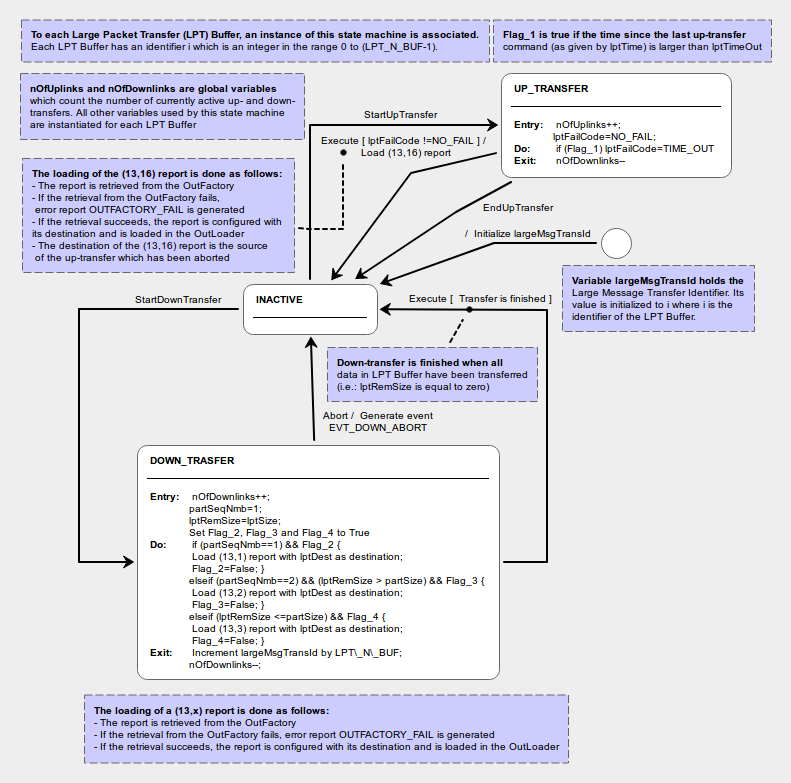
\includegraphics[scale=0.5,keepaspectratio=true]{CrPsLpt.png}
 \caption{Large Packet Transfer (LPT) State Machine}
 \label{fig:LPT}
\end{figure}

To each LPT Buffer, one instance of the LPT State Machine is associated. When no transfer to or from the LPT Buffer is under way, the state machine is in state INACTIVE. 

%----------------------------------------------------------------------
\subsubsection{Management of Down-Transfers}
A down-transfer is started by sending command \textit{StartDownTransfer} to the LPT state machine. In response to this command, the state machine makes a transition to state DOWN\_TRANSFER. The service 13 logic assumes that, at entry into this state, the LPT Buffer has been loaded with the large packet to be down-transferred and that the amount of data to be down-transferred are stored in variable \texttt{lptSize}.

The do-action of the state DOWN\_TRANSFER is responsible for allocating and loading the down-transfer reports (13,1), (13,2) and (13,3).

The collection of the data from the LPT Buffer is done by the Update Action of the service 13 reports. The Update Action is also responsible for updating the \texttt{partSeqNmb} and the \texttt{lptRemSize} variables: every time a service 13 report is executed, \texttt{partSeqNmb} is incremented by 1 and \texttt{lptRemSize} is decremented by \texttt{partSize}. Hence, the normal flow of actions at the starts of a down-transfer (i.e. when the LPT State Machine enters state DOWN\_TRANSFER) is as follows:

\begin{enumerate}
\item The LPT State Machine is executed and the do-action of state DOWN\_TRANSFER creates the OutComponent encapsulating the (13,1) report and loads it in the OutLoader which in turn loads it in the OutManager
\item The OutManager is executed and this causes the OutComponent encapsulating the (13,1) report to be executed.
\item The Update Action of the OutComponent encapsulating the (13,1) report is executed and this causes the first part of down-transfer data to be collected from the LPT Buffer, \texttt{partSeqNmb} to be incremented by 1, and \texttt{lptRemSize} to be decremented by \texttt{partSize}.
\item The (13,1) report is handed over to the middleware for eventual transfer to its destination.
\item The (13,1) report is a one-shot report and it is therefore released after being executed once.
\end{enumerate}

After the first part of the service 13 down-transfer has been processed, the intermediate parts are processed according to the following logic:

\begin{enumerate}
\item The LPT State Machine is executed and the do-action of state DOWN\_TRANSFER creates the OutComponent encapsulating the (13,2) report and loads it in the OutLoader which in turn loads it in the OutManager
\item The OutManager is executed and this causes the OutComponent encapsulating the (13,2) report to be executed.
\item The Update Action of the OutComponent encapsulating the (13,2) report is executed and this causes the next part of down-transfer data to be collected from the LPT Buffer, \texttt{partSeqNmb} to be incremented by 1, and \texttt{lptRemSize} to be decremented by \texttt{partSize}.
\item The (13,2) report is handed over to the middleware for eventual transfer to its destination.
\item The (13,2) report is a repeat report which remains pending for as long as \texttt{lptRemSize} is greater than \texttt{partSize}. Hence, steps 2 to 5 are repeated multiple times until the last intermediate part of the down-transfer is processed.
\end{enumerate}

When \texttt{lptRemSize} has become smaller than \texttt{partSize}, the last part of the down-transfer is processed according to the following logic:

\begin{enumerate}
\item The LPT State Machine is executed and the do-action of state DOWN\_TRANSFER creates the OutComponent encapsulating the (13,3) report and loads it in the OutLoader which in turn loads it in the OutManager
\item The OutManager is executed and this causes the OutComponent encapsulating the (13,3) report to be executed.
\item The Update Action of the OutComponent encapsulating the (13,3) report is executed and this causes the last part of data to be collected from the LPT Buffer and \texttt{lptRemSize} to be decremented by \texttt{partSize}.
\item The (13,3) report is handed over to the middleware for eventual transfer to its destination.
\item The (13,3) report is a one-shot report and it is therefore released after it is executed once.
\item The value of \texttt{lptRemSize} is now zero or negative and this causes the LPT State Machine to make a transition back to state INACTIVE. This marks the end of the down-transfer.
\end{enumerate}

Command \textit{StartDownTransfer} may either originate from the host application (if the host application autonomously decides to start a down-transfer) or it may originate from the private command (13,129). The latter command is provided by the framework to let the user trigger a down-transfer. It takes as an argument the identifier of the LPT Buffer (an integer in the range 1 to LPT\_N\_BUF) from which the down-transfer is to be started.

A down-transfer may be terminated prematurely with command \texttt{Abort}. This causes a transition from DOWN\_TRANSFER to INACTIVE and the generation of event report EVT\_DOWN\_ABORT.

Command \textit{Abort} may either originate from the host application (if the host application autonomously decides to abort a down-transfer) or it may originate from the private command (13,130). The latter command is provided by the framework to let the user abort an on-going down-transfer. The command takes as an argument the Large Message Transfer Identifier of the down-transfer. 

Finally, the LPT State Machine is responsible for managing the nOfDownlinks variable which represents the number of currently on-going down-transfers.

%----------------------------------------------------------------------
\subsubsection{Management of Up-Transfers}
An up-transfer is started by sending command \textit{StartUpTransfer} to the state machine. In response to this command, the state machine makes a transition to state UP\_TRANSFER where it remains until either command \texttt{EndUpTransfer} brings the state machine back to state INACTIVE or the up-transfer is aborted. 

Command \texttt{StartUpTransfer} originates from the (13,9) command which marks the start of an up-transfer. Command \texttt{EndUpTransfer} originates from the (13,11) command which marks the end of the up-transfer.

An up-transfer is aborted if variable \texttt{failCode} holding the failure code becomes set. At entry into state UP\_TRANSFER, this variable is set to NO\_FAIL (nominal value in the absence of failures). This value may change in two ways:

\begin{itemize}
\item If there is a time-out, namely if the time elapsed since the last up-transfer command exceeds \texttt{lptTimeOut}, or
\item If the an up-transfer command is received with a part sequence number which is out-of-sequence.
\end{itemize}

The first condition is evaluated by the do-action of state UP\_TRANSFER. This implies that the resolution of the time-out check is given by the period with which the LPT State Machine is executed. The second condition is evaluated by the start action of the (13,10) and (13,11) commands.

The Progress Action of the up-transfer commands is responsible for copying the data from the command to the LPT Buffer and for updating the variables associated to the LPT Buffer. After the up-transfer is terminated and the LPT State Machine is back in state INACTIVE, application is responsible for processing the data in the LPT Buffer. Note that there is no mechanism to prevent another up-transfer from being started while the application is still busy processing the data in the LPT Buffer. Avoinding this kind of conflicts is a user responsibility.

Finally, the LPT State Machine is responsible for managing the nOfUplinks variable which represents the number of currently on-going up-transfers.


%-------------------------------------------------------------------------------------
\subsection{Service 13 Report and Command Definition}\label{sec:serv13RepCmdDef}
Tables \ref{tab:LptDownFirstRepSpec} to \ref{tab:LptAbortDownCmdSpec} formally specify the service 13 commands and reports by specifying how the actions, checks and attributes of generic out-going commands and reports are specialized for service 13 (see section \ref{sec:defPusRepCmd}). 

\printOutCmpLptDownFirstRepSpec{|c|p{10cm}|}

\newpage
\printOutCmpLptDownInterRepSpec{|c|p{10cm}|}
\printOutCmpLptDownLastRepSpec{|c|p{10cm}|}

\newpage
\printInCmdLptUpFirstCmdSpec{|c|p{10cm}|}
\printInCmdLptUpInterCmdSpec{|c|p{10cm}|}

\newpage
\printInCmdLptUpLastCmdSpec{|c|p{10cm}|}
\printOutCmpLptUpAbortRepSpec{|c|p{10cm}|}

\newpage
\printInCmdLptStartDownCmdSpec{|c|p{10cm}|}
\printInCmdLptAbortDownCmdSpec{|c|p{10cm}|}




%---------------------------------------------------------------------------------
\newpage
\subsection{Service 13 Constants}\label{sec:serv13Const}
The service 13 constants are listed in table \ref{tab:Const-S13}. 

\pnpcsvtable[filter equal={\Domain}{Lpt}]{|p{3cm}|>{\raggedright\arraybackslash}p{9.5cm}|}{Constants for Large Packet Transfer Service}{tab:Const-S13}{Name & Description}{./GeneratedTables/Constants.csv}{\texttt{\Name} & \Desc}


%---------------------------------------------------------------------------------
\subsection{Service 13 Observables and Parameters}\label{sec:serv13Obs}
The service 13 observables and parameters are listed in table \ref{tab:Obs-S13}.

\pnpcsvtable[filter equal={\Domain}{Lpt}]{|p{2.5cm}|c|>{\raggedright\arraybackslash}p{6.5cm}|l|}{Observables and Parameters for LPT Service}{tab:Obs-S13}{Name & Kind & Description & Multiplicity}{./GeneratedTables/Datapool.csv}{\texttt{\Name} & \Kind & \ShortDesc & \Multiplicity}


%----------------------------------------------------------------------------------------
\newpage
\subsection{Service 13 Adaptation Points}
The PUS Extension of the CORDET Framework defines service 13 in full with the exception of the mechanism to access the LPT Buffers. The location of these buffers and the means to access them are application-specific and the framework accordingly defines an Adaptation Point to access these buffers. In a simple case, the adaptation point might take the form of a function which takes the identifier of an LPT Buffer as an argument and whcih returns the start address and size of the buffer itself.

\begin{crAp}{S13}{Adaptation Points for Service 13 (Large Packet Transfer Service)}
\end{crAp}


\newpage
%---------------------------------------------------------------------------------
\subsection{Service 13 Requirements}
The table in this section lists requirements for the test service.

\begin{crReq}{S13}{Requirements for Service 13 (Large Packet Transfer Service)}
\end{crReq}

\begin{figure}[H]
 \centering
 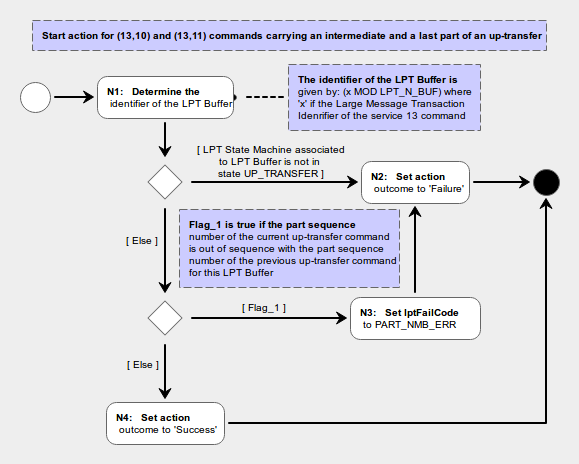
\includegraphics[scale=0.55,keepaspectratio=true]{CrPsCmd13s10Start.png}
 \caption{Up-Transfer Start Action}
 \label{fig:Cmd13s10Start}
\end{figure}




%=============================================================================================
\section{Test Service}\label{sec:serv17}
The service type of the Test Service is 17. The PUS Extension of the CORDET Framework supports this service in full.

The Test Service provides the capability to perform two kinds of connections tests: the \textit{Are-You-Alive Test} and the \textit{On-Board Connection Test}.

The Are-You-Alive test is like a ping test: an external user sends a command of type (17,1) to the application and the application responds by sending to the user a (17,2) report. Neither the (17,1) command nor the (17,2) report carry any parameters. 

In the On-Board-Connection Test, an external user sends a command of type (17,3) to application A asking it to perform a connection test with some other application B. Application B is specified through a parameter carried by the (17,3) command. 

The way the connection test is performed is not specified by the PUS. The PUS Extension of the CORDET Framework implements it as an Are-You-Alive Test from application A to application B. If this Are-You-Alive Test is successful, application A generates a (17,4) report to its user. The Are-You-Alive Test is declared successful if a (17,2) report from application B is received within time \texttt{AreYouAliveTimeOut} from the sending of the (17,1) command.

%=============================================================================================
\subsection{Service 17 Command and Report Definition}
In the CORDET Framework an out-going report is encapsulated in an OutComponent component and an incoming command is encapsulated in an InCommand component. The framework extension accordingly offers the following components to implement the two commands and the two reports of service 17:

\begin{itemize}
\item Component AreYouAliveCmd implements command (17,1) 
\item Component AreYouAliveRep implements report (17,2) 
\item Component OnBoardConnectCmd implements command (17,3)  
\item Component OnBoardConnectRep implements report (17,4) 
\end{itemize}

These components are defined by the way they close the adaptation points of the OutComponent and InCommand. This is defined formally in tables \ref{tab:CR-S17-1} to \ref{tab:CR-S17-4} but the main points are as follows.

The AreYouAliveCmd commmand implements a Progress Action which creates and loads the AreYouAliveRep report. The report destination is the same as the source of the AreYouAliveCmd command. Thus, the processing of the AreYouAliveCmd command consists in sending an AreYouAliveRep to the source of the AreYouAliveCmd. The AreYouAliveCmd commmand is always accepted and it is always started, executed and terminated successfully.

The OnBoardConnectCmd command is always accepted. The command carries as its single parameter the identifier of the application with which the connection test must be performed. The Start Action of the command verifies the legality of this application identifier. In order to establish its legality, service 17 maintains parameter \texttt{onBoardConnectDestLst} to hold the list of legal targets for the On-Board-Connection test. If the application identifier carried by the OnBoardConnectCmd command is not included in this list, its Start Action is deemed to have failed. The Start Action of the OnBoardConnectCmd command is shown in figure \ref{fig:Cmd17s3Start} as an activity diagram.

If, instead, the legality of the target application identifier is confirmed, the Start Action sends an AreYouAliveCmd command to the target application. Normally, the target application should respond by sending it an AreYouAliveRep report. If the expected response (the AreYouAliveRep report) is not received within time \texttt{areYouAliveTimeOut}, the command is deemed to have failed its execution.

The mechanism through which the AreYouAliveRep report notifies the OnBoardConnectCmd command of its arrival is as follows:

\begin{itemize}
\item The service 17 maintains integer variable \texttt{areYouAliveSrc}
\item The Start Action of the OnBoardConnectCmd command resets \texttt{areYouAliveSrc} to zero
\item The Update Action of the incoming report AreYouAliveRep loads its source in variable \texttt{areYouAliveSrc}
\item The Progress Action of the OnBoardConnectCmd command only declares the command to have successfully terminated if, within time-out \texttt{areYouAliveTimeOut}, it finds \texttt{areYouAliveSrc} equal to the identifier of the application with which the connection test is done
\end{itemize}

One implication of this mechanism is that only one On-Board-Connection Test may be active at a given time (i.e. the user should only send a new OnBoardConnectCmd command to an application after execution of the previous OnBoardConnectCmd command has completed). This constraint is not enforced by the framework and is under the responsibility of the user of the service.

The time-out parameter \texttt{areYouAliveTimeOut} is the same for all target applications. There is, in other words, an underlying assumption that the response time of all target applications is similar and that there is therefore no need to maintain separate time-outs for each target application. If this assumption is not satisfied, the user must update the value of \texttt{areYouAliveTimeOut} before starting an On-Board-Connection Test.

Tables \ref{tab:CR-S17-1} to \ref{tab:CR-S17-4} formally specify the service 17 commands and reports by specifying how the actions, checks and attributes of generic out-going commands and reports are specialized for service 17 (see section \ref{sec:defPusRepCmd}). The following considerations apply to the service 17 commands and reports:

\begin{itemize}
\item The service 17 commands execute in 'one-shot' mode and therefore do not generate progress reports.
\item Service 17 reports are generated unconditionally and hence their enable check always returns 'report enabled'.
\item Service 17 reports are generated as soon as the condition which triggered them occur and hence their ready check always returns 'ready'
\item Service 17 reports are 'one-off' reports and hence their repeat check always returns 'no repeat'
\end{itemize}

\newpage
\printInCmdTstAreYouAliveCmdSpec{|c|p{10cm}|}
\printOutCmpTstAreYouAliveRepSpec{|c|p{10cm}|}

\newpage
\printInCmdTstConnectCmdSpec{|c|p{10cm}|}
\printOutCmpTstConnectRepSpec{|c|p{10cm}|}



%---------------------------------------------------------------------------------
\newpage
\subsection{Service 17 Constants}\label{sec:serv17Const}
The service 17 constants are listed in table \ref{tab:Const-S17}. 

\pnpcsvtable[filter equal={\Domain}{Lpt}]{|p{3cm}|>{\raggedright\arraybackslash}p{9.5cm}|}{Constants for Test Service}{tab:Const-S17}{Name & Description}{./GeneratedTables/Constants.csv}{\texttt{\Name} & \Desc}

%---------------------------------------------------------------------------------

\subsection{Service 17 Observables and Parameters}\label{sec:serv17Obs}
The service 17 observables and parameters are listed in table \ref{tab:Obs-S13}.

\pnpcsvtable[filter equal={\Domain}{Tst}]{|p{4cm}|c|>{\raggedright\arraybackslash}p{7.5cm}|}{Observables and Parameters for Test Service}{tab:Obs-S17}{Name & Kind & Description}{./GeneratedTables/Datapool.csv}{\texttt{\Name} & \Kind & \ShortDesc}


%---------------------------------------------------------------------------------
\subsection{Service 17 Requirements}
The table in this section lists requirements for the test service.

\begin{crReq}{S17}{Requirements for Service 17 (Test Service)}
\end{crReq}

\newpage
\begin{figure}[H]
 \centering
 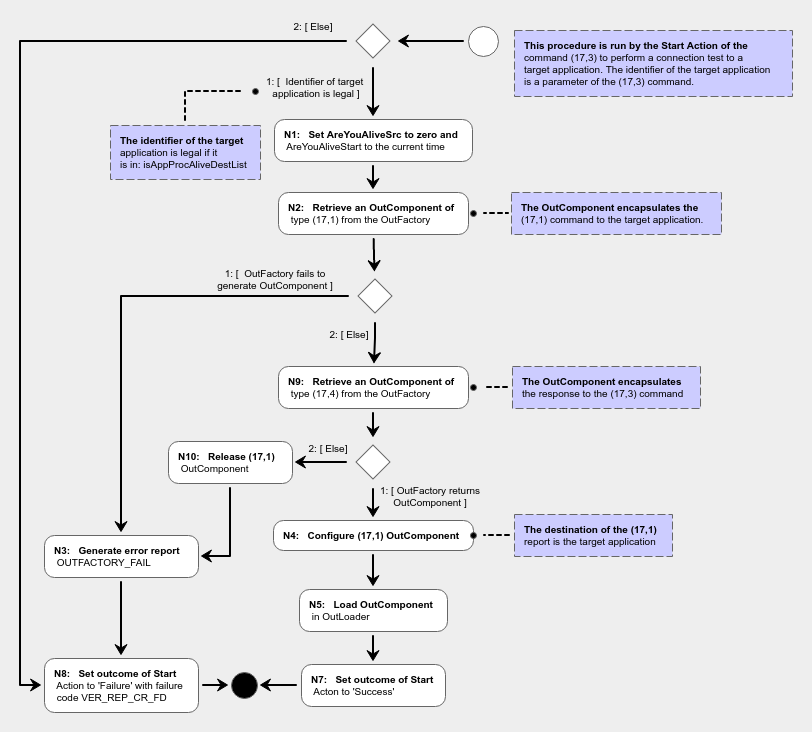
\includegraphics[scale=0.415,keepaspectratio=true]{CrPsCmd17s3Start.png}
 \caption{Start Action of OnBoardConnectCmd (17,3) Command}
 \label{fig:Cmd17s3Start}
\end{figure}

\begin{figure}[H]
 \centering
 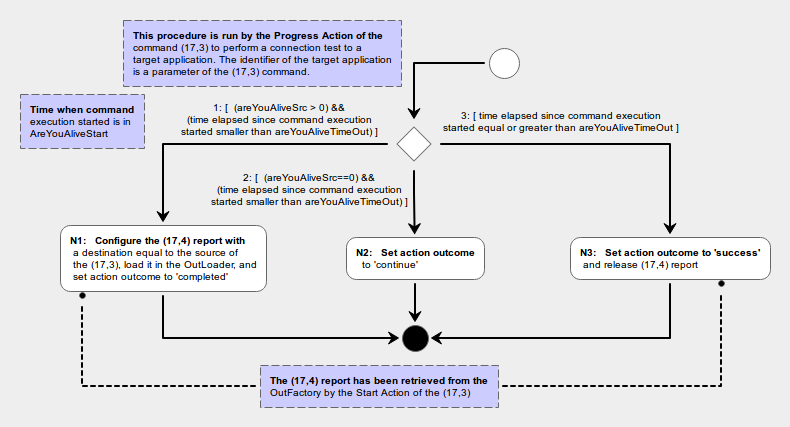
\includegraphics[scale=0.415,keepaspectratio=true]{CrPsCmd17s3Prgr.png}
 \caption{Progress Action of OnBoardConnectCmd (17,3) Command}
 \label{fig:Cmd17s3Prgr}
\end{figure}


%=============================================================================================
\section{Event Action Service}\label{sec:serv19}
The specification of this service is still TBD.



\newpage
\appendix
%=============================================================================================
\section{Pre-Defined Event Reports}\label{sec:preDefEvtRep}
The table in this section lists all the service 5 event reports which are generated by components of the PUS Extension of the CORDET Framework. For each event report, the following information is provided:

\begin{itemize}
\item The name of the event report
\item The description of the event report
\item The parameters carried by the event report
\end{itemize}

\begin{landscape} 

\pnpcsvtable{|c|>{\raggedright\arraybackslash}p{9cm}|>{\raggedright\arraybackslash}p{9cm}|}{Event Reports}{tab:evtRep}{Name & Description & Parameters}{./GeneratedTables/PUSExtensionCrPsEvtIdt.csv}{\texttt{\Name} & \Description & \Parameters}

\end{landscape}


%=============================================================================================
\section{Error Reports}\label{sec:errRep}
The table in this section lists all the error reports which are generated by the PUS Extension of the CORDET Framework. For each error report, the following information is provided:

\begin{itemize}
\item The name of the error report
\item The description of the error report
\item The parameters carried by the error report
\end{itemize}

\begin{landscape} 


\pnpcsvtable{|c|>{\raggedright\arraybackslash}p{9cm}|>{\raggedright\arraybackslash}p{8cm}|}{Error Reports}{tab:evtRep}{Name & Description & Parameters}{./GeneratedTables/PUSExtensionCrPsErrRepCodet.csv}{\texttt{\Name} & \Description & \ErrRepData}


\end{landscape}

%=============================================================================================
\section{Request Verification Failure Codes}\label{sec:reqVerFailCodes}
Request verification failure reports of service 1 carry a failure code. The table in this section lists all the failure codes supported by the PUS Extension of the CORDET Framework. Failure reports carry parameters. Some of these parameters are common to all failure reports but the Failure Verification Data is code-specific (see section \ref{sec:serv1RepDef}). This is defined in the rightmost column of the table.

\begin{landscape}

\pnpcsvtable{|l|p{11cm}|>{\raggedright\arraybackslash}p{6cm}|}{Request Verification Failure Codes}{tab:reqVerFailCodes}{Name & Description & Ver. Failure Data}{./GeneratedTables/PUSExtensionCrPsFailCodet.csv}{\texttt{\Name} & \Description & \verFailData}

\end{landscape}



%=============================================================================================
\section{PUS Requirements Compliance Matrix}\label{sec:PusReqSOC}
The table in this section presents the level of compliance achieved by the PUS Extension of the CORDET Framework to the PUS requirements of AD-1. The first three columns give the identifier, the title and the text of the PUS requirement. The fourth column gives the compliance status which can be one of the following:

\begin{itemize}
\item [C1] The requirement is directly implemented by the PUS Extension of the CORDET Framework or by the CORDET Framework itself (i.e. applications instantiated from the framework are guaranteed to be compliant with the requirement)
\item [C2] The requirement may be implemented by applications instantiated from the PUS Extension of the CORDET Framework (i.e. applications instantiated from the framework may be made be compliant with the requirement)
\item [NC] The requirement is not compatible with the PUS Extension of the CORDET Framework (i.e. applications instantiated from the framework cannot be compliant with the requirement)
\item [NA] The requirement is not covered by the PUS Extension of the CORDET Framework
\end{itemize}

In several cases, the compliance level is declared to be 'C1/C2' when part of the requirement is implemented by the PUS Extension of the CORDET Framework and part is left to the application developers.

The fourth column in the table provides a discussion of the level of compliance and, wherever possible, the following additional information is provided:

\begin{itemize}
\item [C1] Traceability to the framework requirements implementing the PUS requirement 
\item [C2] Traceability to the adaptation point(s) where application developers can insert their own requirements to achieve compliance
\item [NC] Justification for non-compliance
\item [NA] Explanation of the reason for the non-applicability of the requirement
\end{itemize}

Only requirements in sections 5 to 7 of the PUS are covered. Requirements in section 8 merely state the layout of the standard commands and reports. Compliance to these requirements is uncontroversial and is guaranteed in all cases. Requirements in section 9 are not relevant to the PUS Extension of the CORDET Framework and are therefore ignored.

\begin{landscape} 

\pnpcsvtable{|c|>{\raggedright\arraybackslash}p{3.0cm}|>{\raggedright\arraybackslash}p{7cm}|c|>{\raggedright\arraybackslash}p{7cm}|}{Mapping of PUS Requirements to CORDET Requirement}{tab:mappingPusToCr}{N & Title & Requirement & C & Justification}{PusCompliance.csv}{\ReqN & \ReqTitle & \ReqText & \Status & \Justification}


\end{landscape}




\end{document}  




